%%% Local Variables:
%%% mode: latex
%%% TeX-master: t
%%% End:

%\documentclass[doctor,secret]{ucasthesis}
\documentclass[master,secret]{ucasthesis}
%\documentclass[doctor]{ucasthesis}
% \documentclass[%
%   master|doctor, % mandatory option
%   secret,
%   arialtoc,arialtitle]{ucasthesis}

% 所有其他可能用到的包都统一放到这里了,可以根据自己的实际添加或者删除。
\usepackage{ucastils}
\usepackage{bm}
\usepackage{algorithm}
\usepackage{algorithmic}
\usepackage{extarrows}
\usepackage{bbding}
% 你可以在这里修改配置文件中的定义,导言区可以使用中文。
% \def\myname{朝鲁}

\begin{document}

% 定义所有的eps文件在 figures 子目录下
\graphicspath{{figures/}}

%%% 封面部分
\frontmatter

%%% Local Variables:
%%% mode: latex
%%% TeX-master: t
%%% End:
%\secretcontent{\heiti 绝密}
\secretcontent{}

\ctitle{面向图像集合分类的黎曼流形判别学习方法研究}
% 根据自己的情况选,不用这样复杂
\makeatletter

\makeatother

%\cdegree{{\heiti 工学硕士}}
%\cdepartment[计算所]{{\heiti 中国科学院计算技术研究所}}
%\cmajor{{\heiti 计算机科学与技术}}
%%\cauthor{朝\hspace{1em}鲁} 
%\cauthor{{\heiti 李显求}}
%\csupervisor{{\heiti 陈熙霖\hspace{1em}研究员}}
%\csupervisorplace{{\heiti 中国科学院计算技术研究所}}
\cdegree{工学硕士}
\cdepartment[计算所]{中国科学院计算技术研究所}
\cmajor{计算机科学与技术}
%\cauthor{朝\hspace{1em}鲁} 
\cauthor{李显求}
\csupervisor{陈熙霖\hspace{1em}研究员}
\csupervisorplace{中国科学院计算技术研究所}
% 如果没有副指导老师或者联合指导老师,把下面两行相应的删除即可。


% 日期自动生成,如果你要自己写就改这个cdate
%\cdate{\CJKdigits{\the\year}年\CJKnumber{\the\month}月}
%\cdate{\textbf{\the\year{\heiti 年}\the\month{\heiti 月}}}
\cdate{\the\year 年\the\month 月}

% 博士后部分
% \cfirstdiscipline{计算机科学与技术}
% \cseconddiscipline{系统结构}
% \postdoctordate{2009年7月——2011年7月}

\etitle{Discriminant Learning on Riemannian Manifold for Image Set Classification}
% 这块比较复杂,需要分情况讨论:
% 1. 学术型硕士
%    \edegree:必须为Master of Arts或Master of Science(注意大小写)
%              “哲学、文学、历史学、法学、教育学、艺术学门类,公共管理学科
%               填写Master of Arts,其它填写Master of Science”
%    \emajor:“获得一级学科授权的学科填写一级学科名称,其它填写二级学科名称”
% 2. 学术型博士
%    \edegree:Doctor of Philosophy(注意大小写)
%    \emajor:“获得一级学科授权的学科填写一级学科名称,其它填写二级学科名称”

\edegree{Master of Science}
\eauthor{Li Xianqiu}
\edepartment{Institute of Computing Technology\\Chinese Academy of Sciences}
\emajor{Computer Science and Technology}
\esupervisor{Chen Xilin}

% 这个日期也会自动生成,你要改么?
% \edate{December, 2005}

% 定义中英文摘要和关键字
\begin{cabstract}
视觉作为人类的主要的感知机能之一,对人类感知世界的重要性不言而喻。计算机视觉的任务就是为计算机赋予接近甚至超过人类视觉的感知能力。图像作为计算机视觉任务的主要输入,与其它数据形式(如文本,语音等)相比蕴含了更多的信息。

另一方面尽管图像本身蕴含了丰富的信息但是如何运用这些信息,以及图像本身的一些问题(如视角变化大、光照变化剧烈、分辨率低等)也给视觉任务带来不小的挑战。与此同时,越来越多现实生活中的数据以集合的形式出现:视频监控数据、用户上传视频、主题相册、物体的多视角数据以及动作描述视频等在近年来都呈现出爆发式的增长;图像集合分类问题也在这样的背景下应运而生,针对集合中的数据呈现出的量大但质未必优的特点,图像集合分类问题的核心任务之一便是利用数据量大的特点以克服质低的问题。经过10多年的发展,根据图像集合的表示方式的不同,图像集合分类相关方法逐渐形成了以下的一些类别:1、子空间以及流形建模的方法;2、仿射包建模的方法;3、统计建模的方法;4、深度学习的方法;5、其它(稀疏编码,协同表示等)。

在众多方法中,统计建模的方法以其优越表现逐渐成为研究该问题的主要方法之一,本文将以黎曼流形为工具对统计建模图像集合问题进行研究。本文的主要工作包含:1)研究了矩阵函数与流形上的优化理论与方法,在对流形、矩阵函数等概念介绍的基础上,对矩阵流形上的优化问题进行探讨,并结合学位论文课题中的实例对矩阵流形优化进行介绍,一方面帮助读者理解并复现本文所提出的方法,另一方面也为解决类似优化问题提供借鉴。2)提出了黎曼流形上的偏最小二乘回归方法,通过借助切空间构建子流形的方式将欧氏空间中的偏最小二乘回归(Partial Least Square Regression, PLSR)扩展到黎曼流形;并考虑到黎曼流形与欧氏空间的几何结构差异以及图像集合数据稀疏的问题,进一步设计了借助多切空间构建子流形的方法,采用逐步回归的策略整合多个切空间中的结果;本文以非奇异协方差矩阵即对称正定矩阵(Symmetric Positive Definite, SPD)黎曼流形为实例,在集合数据分类问题上进行了实验,取得了与当前最优方法可比甚至更好的结果。3)提出了低秩对称半正定矩阵(Low-Rank symmetric Positive Semi-Definite, PSD)建模图像集合的方法,解决样本协方差矩阵建模图像集合时由于数据稀疏带来的矩阵奇异(不满秩)、由于噪声带来的矩阵估计不准、以及对称正定矩阵表示时空开销大等问题;并采用图嵌入(Graph Embedding)的方法将判别信息内嵌到的低秩对称半正定矩阵表示中,最后在核判别分析(Kernel Discriminant Analysis, KDA)的框架下研究了该表示下的判别学习问题,并验证了低秩对称半正定矩阵表示的有效性。

%  论文的摘要是对论文研究内容和成果的高度概括。摘要应对论文所研究的问题及其研究目
%  的进行描述,对研究方法和过程进行简单介绍,对研究成果和所得结论进行概括。摘要应
%  具有独立性和自明性,其内容应包含与论文全文同等量的主要信息。使读者即使不阅读全
%  文,通过摘要就能了解论文的总体内容和主要成果。
%
%  论文摘要的书写应力求精确、简明。切忌写成对论文书写内容进行提要的形式,尤其要避
%  免“第 1 章……;第 2 章……;……”这种或类似的陈述方式。
%
%  本文介绍中国科学院大学论文模板 \ucasthesis{} 的使用方法。本模板符合学校的硕士、
%  博士论文格式要求。
%
%  本文的创新点主要有:
%  \begin{itemize}
%    \item 用例子来解释模板的使用方法;
%    \item 用废话来填充无关紧要的部分;
%    \item 一边学习摸索一边编写新代码。
%  \end{itemize}
%
%  关键词是为了文献标引工作、用以表示全文主要内容信息的单词或术语。关键词不超过 5
%  个,每个关键词中间用分号分隔。(模板作者注:关键词分隔符不用考虑,模板会自动处
%  理。英文关键词同理。)
\end{cabstract}

\ckeywords{图像集合;统计建模;黎曼流形;判别学习}

\begin{eabstract} 
Vision functionality serves as one of the main abilities for human to percept the real world, and its importance goes without saying. The mission of CV (Computer Vision) is to endow computers with close to or even stronger ability than human to perceive the real world. 

As the main input for CV tasks, images contain much more information than text, audio and so on, but how to make full use of the information becomes a problem. The variations of images bring great challenges to CV tasks. At the same time, data comes more frequently in the form of image set, such as surveillance video, multi-view image sets and so on. Under these background, image set classification comes into being. Image sets usually contain a large amount of images in poor quality. So one major task in image set classification is to overcome the disadvantage of low quality and leverage the advantage of large quantity. 

With more than ten years of development, a lot of methods have been proposed for this task. According to how to model an image set they can be divided into following categories: 1. Subspace/Manifold based methods, 2. Affine hull based methods, 3. Statistics model based methods, 4. Deep Learning based methods. 5. Others, like Dictionary/Sparse coding based method, Collaborative representation methods, etc.

Among the categories listed above, Statistics model based methods have attracted a lot attention with its excellent performance. This thesis takes Riemannian manifold as basic tool and tries to explore statistics model based methods. The main contributions include: 1) Studied matrix function and manifold optimization theory and methods. By introducing the basic concept of manifold and matrix function, along with the real-world problems extracted from the following research topics, optimization algorithms on the manifold have been studied in this thesis (Chapter 2). On the one hand it will help readers understand and implement methods proposed in this thesis, and on the other hand it can also provide basic instructions to solve other similar problems. 2) Proposed Partial Least Square Regression methods on Riemannian manifold with sub-manifold constructed from one tangent space (usually taking the tangent space of samples’ Karcher mean). Then in order to overcome the structure difference between Euclidean space and Riemannian manifold as well as the drawback of sparse sampling, multi-tangent space Partial Least Square Regression method has been designed. On the Symmetric Positive Definite (SPD) matrices manifold, image set classification experiment were designed to evaluate the proposed method and it is observed that the proposed method is comparable or even outperforms the state-of-art methods on the commonly used databases. 3) Proposed Low-Rank PSD matrices based image set model to overcome the rank-deficient and high dimension problems of sample covariance models as well as lack of scale information (eigenvalue) drawback in the subspace models. With Graph Embedding framework we encoded label information into Low-Rank PSD (Low-Rank symmetric Positive Semi-Definite) representations of image sets and then designed the discriminant learning methods with Kernel Discriminant Analysis framework. Experiments on the commonly used databases has shown to support our proposition.

%   An abstract of a dissertation is a summary and extraction of research work
%   and contributions. Included in an abstract should be description of research
%   topic and research objective, brief introduction to methodology and research
%   process, and summarization of conclusion and contributions of the
%   research. An abstract should be characterized by independence and clarity and
%   carry identical information with the dissertation. It should be such that the
%   general idea and major contributions of the dissertation are conveyed without
%   reading the dissertation. 
%
%   An abstract should be concise and to the point. It is a misunderstanding to
%   make an abstract an outline of the dissertation and words ``the first
%   chapter'', ``the second chapter'' and the like should be avoided in the
%   abstract.
%
%   Key words are terms used in a dissertation for indexing, reflecting core
%   information of the dissertation. An abstract may contain a maximum of 5 key
%   words, with semi-colons used in between to separate one another.
\end{eabstract}

\ekeywords{Image set, Statistics model, Riemannian manifold, Discriminant learning}

% 设置 PDF 文档的作者、主题等属性
\makeatletter
\ucas@setup@pdfinfo
\makeatother
\makecover

% 目录
\tableofcontents
% 插图索引
\listoffigures
% 表格索引
\listoftables
% 符号对照表
%\begin{denotation}

\item[HPC] 高性能计算 (High Performance Computing)
\item[cluster] 集群
\item[Itanium] 安腾
\item[SMP] 对称多处理
\item[API] 应用程序编程接口
\item[PI]	聚酰亚胺
\item[MPI]	聚酰亚胺模型化合物,N-苯基邻苯酰亚胺
\item[PBI]	聚苯并咪唑
\item[MPBI]	聚苯并咪唑模型化合物,N-苯基苯并咪唑
\item[PY]	聚吡咙
\item[PMDA-BDA]	均苯四酸二酐与联苯四胺合成的聚吡咙薄膜
\item[$\Delta G$]  	活化自由能~(Activation Free Energy)
\item [$\chi$] 传输系数~(Transmission Coefficient)
\item[$E$] 能量
\item[$m$] 质量
\item[$c$] 光速
\item[$P$] 概率
\item[$T$] 时间
\item[$v$] 速度
\item[劝  学] 君子曰:学不可以已。青,取之于蓝,而青于蓝;冰,水为之,而寒于水。
  木直中绳。(车柔)以为轮,其曲中规。虽有槁暴,不复挺者,(车柔)使之然也。故木
  受绳则直, 金就砺则利,君子博学而日参省乎己,则知明而行无过矣。吾尝终日而思
  矣,  不如须臾之所学也;吾尝(足齐)而望矣,不如登高之博见也。登高而招,臂非加
  长也,  而见者远;  顺风而呼,  声非加疾也,而闻者彰。假舆马者,非利足也,而致
  千里;假舟楫者,非能水也,而绝江河,  君子生非异也,善假于物也。积土成山,风雨
  兴焉;积水成渊,蛟龙生焉;积善成德,而神明自得,圣心备焉。故不积跬步,无以至千
  里;不积小流,无以成江海。骐骥一跃,不能十步;驽马十驾,功在不舍。锲而舍之,朽
  木不折;  锲而不舍,金石可镂。蚓无爪牙之利,筋骨之强,上食埃土,下饮黄泉,用心
  一也。蟹六跪而二螯,非蛇鳝之穴无可寄托者,用心躁也。—— 荀况
\end{denotation}


%%% 正文部分
\mainmatter
% 这是前沿和背景的一章,主要会介绍对于该问题的研究的意义以及,目前的一些研究状况
\chapter{绪\hspace{1em}论}
\label{cha:intro}
宋代诗人苏东坡说过:“博观而约取,厚积而薄发”。意思是说,只有广见博识才能择其精者而取之。研究如此,研究生生涯亦是如此。研究生生涯作为人生的一部分,从长远来看是一个厚积的过程,这个时期积累的对待问题的态度,见识的众多同行的思想碰撞以及研究过程中的失败与成功等,都会成为今后生活的财富;而短期内,也就是落实到研究中,只有充分调研了问题的背景,了解了国内外了情况并取其精华去其糟粕,准备了充分的数据才能在自己的实际工作中得心应手,做出期望的成果。

绪论作为文章的开始,将为学位论文的展开作铺垫,引领读者进入本文的研究领域——图像集合分类问题。为此,本章首先会对问题的背景和意义进行简要的说明,让读者对该问题在国内外的研究现状有个整体把握的同时,对该问题的测试数据和测试协议也有一个大致的了解,最后借助对本文的主体框架的介绍,让读者对文章的结构有一个宏观的把握。
\section{问题的背景与意义}
\label{sec:background}
计算机视觉的任务就是希望给机器赋予等同甚至是超过人类视觉系统对于周围环境的处理能力。图像作为计算机视觉的主要输入,为计算机理解提供丰富信息的同时也给计算机视觉任务带来了挑战:首先,图像是三维空间向二维空间的投影,大量的信息在这个过程中丢失;其次,由于拍摄的角度变化,光照变化以及低分辨率,遮挡等问题使得用单一的图像进行识别、理解等任务变得十分困难;另一方面,由于近年来监控视频,主题相册,用户上传视频,多视角图像数据等都以图像集合的形式呈现出爆发式的增长。利用集合数据的优势克服以上一些问题逐渐成为了一种趋势,图像集合分类问题在这样的大背景下应运而生。

图像集合分类问题的中的数据的主要呈现出两个特点:一是图像的量大,二是图像的质却未必优(variation大)。因而图像集合分类问题的主要任务就是利用量大的特点克服variation大的问题。由于以上的原因,加之数据本身以集合的形式呈现的特点为图像集合分类问题的研究赋予了重要的实践和理论意义。

计算机视觉的任务的大多来源于实际问题的,图像集合的分类也不例外,视频监控就是一个很好的例子,视频监控中的分类识别问题对于警方的网络追逃,海关的出入境管理等的重要性不言而喻;此外,动作识别(动作的描述往往是一段视频输入)对于暴力事件的甄别,预防犯罪也有重要的意义;另一方面,在众多的用户上传的视频数据中不管是做基本的视频检索还是做更深层次的用户行为的分析理解等,图像集合分类问题的研究同样具有重要的意义。

在理论上图像集合分类问题的意义主要体现在:首先,图像数据中的数据是以集合的形式存在,相较于机器学习领域的中的单点(向量)的研究,集合作为输入的研究却不是那么充分;所以图像集合的分类问题的研究对于机器学习中的集合对象的研究有着一定的推动意义;其次,由于数据的独特性,其数学表示也比较特殊,往往是子空间,对称正定矩阵,分布函数,流形等。而这些非线性结构的表示的研究也将促进机器学习中非线性数据表示的研究。
\section{国内外研究现状}
\label{sec:current}
本节将针对图像集合分类问题在国内外的研究现状进行介绍,帮助读者了解该问题的前沿动态,理解图像集合分类问题本身以及该问题的核心任务和主流的解决方案。
\subsection{符号说明}
\label{sec:symbols}
在进入本节的主要内容之前,由于本文涉及较多数学符号;为了节约篇幅,这里利用表\ref{tab:symbols}统一对本文中的主要符号进行说明。并且本文约定:如无特别说明将使用小写字母(如:$a,b$)表示常量,小写加粗(如:$\bm{x},\bm{y}$)表示向量,大写的字母(如:$X,Y$)表示矩阵,子空间或集合(具体可根据上下文确定),大写字母加粗(如:$\bm{X},\bm{Y}$)表示张量。
\begin{table}[htb]
  \centering
  \begin{minipage}[t]{0.8\linewidth} % 如果想在表格中使用脚注,minipage是个不错的办法
  \caption{符号说明}
  \label{tab:symbols}
    \begin{tabular*}{\linewidth}{lp{10cm}}
      \toprule[1.5pt]
      {\heiti 符号} & {\heiti 说明} \\\midrule[1pt]
      $\mathbb{R}^{n}$ & $n$维向量空间,特别地$\mathbb{R}$表示实数空间 \\
      $M$ & 此符号专用于表示流形(Manifold)\\
      $(S,g)$ &表示黎曼流形(集合$S$以及其上的黎曼度量$g$的二元组),通常为了简单起见也用$S$代表该流形(如用$\mathbb{S}_{d}^{+}$表示对称正定矩阵流形),因此$S$的具体意义需要根据上下文确定\\
      $\mathbb{S}_{d}^{+}$ & $d \times d$的对称正定矩阵集合(SPD矩阵)\\
      $\mathbb{S}_{d}^{+}(k)$    & 秩为$k$的$d \times d$半正定矩阵集合(Fixed-Rank PSD矩阵)\\
      $\mathbb{S}_{d}$ & $d \times d$的对称矩阵构成的集合\\
      ${\rm St}(n,k)$   & non-compact Stiefel流形,定义在$n \times k$列满秩矩阵的集合上\\
      ${\rm St}^{*}(n,k)$   & compact Stiefel流形,定义在$n \times k$列正交矩阵的集合上\\
      ${\rm Gr}(n,k)$   & Grassmann流形,定义在$\mathbb{R}^{n}$中$k$维子空间构成的集合上\\
      $\log(\cdot)$ & 不做特别说明的话本文中表示的是矩阵的$\log$函数\\
      $\exp(\cdot)$ & 不做特别说明的话本文中表示的是矩阵的$\exp$函数\\
      ${\rm Log}$ & 流形上的${\rm Log}$变换\\
      ${\rm Exp}$ & 流形上的${\rm Exp}$变换\\
      $R$ & 流形上的Retraction变换\\
      ${\rm T}$ & 流形上的Vector Transport变换\\
      $T_{X}M$ & 流形$M$上$X$处的切空间(tangent space)。特别地,$M$上的所有切空间记为$TM$称为$M$上的切空间束\\
      \bottomrule[1.5pt]
    \end{tabular*}
  \end{minipage}
\end{table}
\subsection{图像集合}
\label{sec:Image-Set}
图像集合,顾名思义指的就是多张图片构成的集合,其已经被用于多个领域(视频人脸识别,物体识别,动作识别,表情识别等等),图\ref{fig:image_set_exmples}给出了几个例子。
\begin{figure}[h]
	\subcaptionbox{EXAMP 01: 一段录像\label{fig:subfig_facetrack}(图片来自YTC\cite{Database_YTC}数据库)}
      	{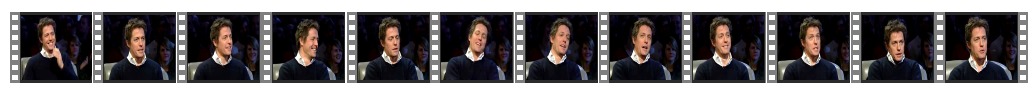
\includegraphics[width=\linewidth]{source/YTC_track.png}}
  	\subcaptionbox{EXAMP 02: 一个物体的Multi-view\label{fig:subfig_apple}(图片来自ETH80\cite{Database_ETH80}数据库)}
      	{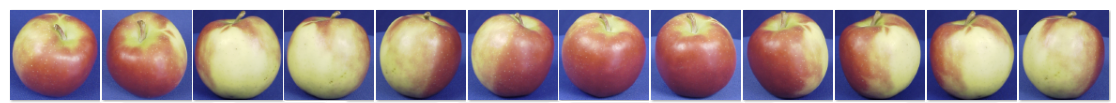
\includegraphics[width=\linewidth]{source/ETH80_apple.png}}
  	\subcaptionbox{EXAMP 03:一个动作描述\label{fig:subfig_motion}(图片来自CMU MoBo\cite{Database_MoBo}数据库)}
    	{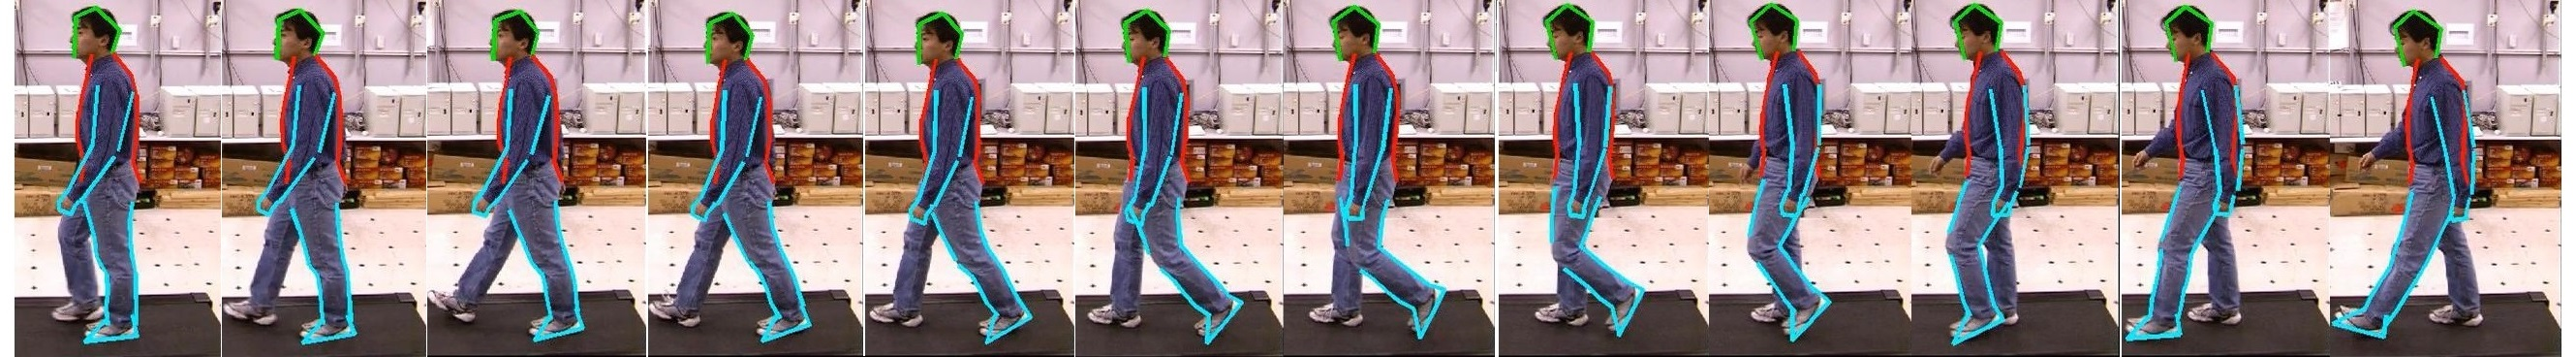
\includegraphics[width=\linewidth]{source/cmu_MoBo.jpg}}
  	\caption{几个图像集合的例子}
  	\label{fig:image_set_exmples}
\end{figure}

图像集合的分类问题的研究和发展已经走过了10多年的时间;在这10多年中,图像集合分类问题从最初被引入CV领域,逐渐成为计算机视觉中的一个研究热点;这个过程中,学者们不断推陈出新,发展出了一系列的方法和路线,为图像集合分类问题的研究做出了重要的探索。

首先,从问题层面可以将图像集合分类问题分为两个大类:图像集合对图像集合的分类问题(Probe和Gallery都是图像集合,在图像集合分类问题中Probe相当于测试集而Gallery相当于训练集),图像集合对静态图像的分类问题(Probe和Gallery中一边是静态图像另一边是图像集合)。其中前者是目前图像集合分类问题研究的主流方向,而后者则是一个新的方向,拥有着广泛的运用前景,在该方向上的一些主要工作有:文献\cite{Statistics_LERM}探究了静态图像到图像集合的分类问题;文献\cite{Statistics_HER}则把静态图像与图像集合的匹配的问题开创性的运用到了视频/图像检索领域;而文献\cite{Affinehull_P2SML}借助Affine Hull表示图像集合,在Metric Learning的框架下,比较全面的讨论了point-to-set以及set-to-set的问题。

图像集合到图像集合的分类问题一直以来是图像集合分类问题的主流的方向,这个问题上按照方法这里进一步的可把图像集合分类问题归纳为如下的几类:1、子空间以及流形建模的方法\cite{Subspace_MSM,Subspace_GDA,Manifold_MMD,Manifold_MDA};2、仿射包建模的方法\cite{Affinehull_AF,Affinehull_SANP,Affinehull_RNP,Affinehull_ProNN};3、统计建模的方法\cite{Statistics_CDL,Statistics_Vemu,Statistics_SPDML,Statistics_LMKML,Statistics_HERML,Statistics_DARG,Statistics_BeyondGauss};4、深度学习的方法\cite{Deeplearning_MMDML,Deeplearning_DRM};5、其它(稀疏编码\cite{Collaborative_ISBCOLREP},协同表示\cite{Dictionary_DBFR}等)。接下来的内容将简要对它们进行介绍。
\subsection{子空间以及流形建模的方法}
\label{sec:current_Subspace_Manifold}
这一类方法出现在图像集合问题研究的早期,为图像集合问题的形成奠定了基础,并且为该问题给出了早期的解决方案。
\subsubsection{子空间建模的方法}
\label{sec:current_SubMan_Subspace}
工作\cite{Subspace_MSM},\cite{Subspace_GDA}是使用子空间建模图像集合的代表,工作\cite{Subspace_MSM}提出了使用图像集合来克服图像大variation的问题(以量取胜),并使用子空间建模图像集合,然后使用主夹角来进行距离度量,工作\cite{Subspace_GDA}进一步的研究了子空间的方法,并且将其统一到Grassmann流形下进行解释。子空间建模图像集合的算法流程可以大致概括如下(参考\cite{Subspace_GDA}):
\begin{itemize}
\item 设$\{\bm{x}_{ij} \in \mathbb{R}^{d}\}_{j=1}^{n_i}$表示第$i$个图像集合,其中$n_i$表示的是集合中的样本数
\item 计算样本均值:$\bar{\bm{x}}_i=\frac{1}{n_i}\sum_{i=1}^{n_i} \bm{x}_{ij}$,样本协方差:$C_i=\frac{1}{n_i-1}\sum_{j=1}^{n_i}(\bm{x}_{ij}-\bar{\bm{x}}_i)(\bm{x}_{ij}-\bar{\bm{x}}_i)^{T}$
\item 对样本协方差做奇异值分解获得:$C_i=U_i\Lambda_iU_{i}^{T}$,指定子空间维数$m(m<d)$,这里假设奇异值分解的结果是按特征值由大到小排序的
\item 获得集合的子空间表示:$Y_i=U_i(:,1:m)$,其中$U_i(:,1:m)$表示取$U_i$的前$m$列
\item 定义两个子空间之间的距离,用于度量$\{Y_j\}_{j=1}^n$的两两之间的距离;在子空间的度量中,主夹角是最主要的概念:
\begin{equation}
\label{principal_angle}
\begin{split}
&\cos \theta_{k}=\max_{\bm{u}_k \in {\rm span(Y_i)}}\max_{\bm{v}_k \in {\rm span(Y_j)}} \bm{u}_{k}^{T}\bm{v}_{k}\\
&~~~~~~~s.t~~\bm{u}_{k}^{T}\bm{u}_{k}=1,\bm{v}_{k}^{T}\bm{v}_{k}=1\\
&\bm{u}_{k}^{T}\bm{u}_{i}=0,\bm{v}_{k}^{T}\bm{v}_{i}=0,(i=1,2,...,k-1)\\
\end{split}
\end{equation}
其物理意义图\ref{fig:principle_angle}所示。
\begin{figure}[h]
	\centering
	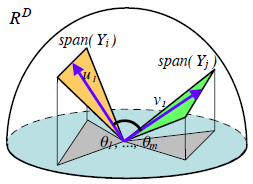
\includegraphics[width=0.4\linewidth]{source/principal_angle.png}
	\caption[子空间之间的主夹角示意图]{子空间之间的主夹角示意图(图片来自文献\cite{Subspace_GDA})}
	\label{fig:principle_angle}
\end{figure}
\item 利用主夹角定义子空间中的距离度量:\\
Projection metric: $d_p (Y_i,Y_j)=\left(∑_{i=1}^m \sin^2 \theta_i\right)^{\frac{1}{2}}$\\
Max correlation: $d_{Max} (Y_i,Y_j)=\left(1-\cos^2\theta_1\right)^\frac{1}{2}$\\
Min correlation: $d_{Min} (Y_i,Y_j)=\left(1-\cos^2\theta_m\right)^\frac{1}{2}$\\
Procrustes metric: $d_{CF} (Y_i,Y_j)=2\left(∑_{i=1}^{m}\sin^2(\theta_i/2)\right)^\frac{1}{2}$
\end{itemize}

工作\cite{Subspace_GDA}进一步在此基础上利用核判别分析(Kernel Discriminant Analysis, KDA)的框架进行了判别学习,在核空间中进行图像集合的分类。
\subsubsection{流形建模的方法}
\label{sec:current_SubMan_Manifold}
流形建模的方法\cite{Manifold_MMD},\cite{Manifold_MDA}假设图像集合中的图像位于流形上(并不充满整个空间),使用多个局部线性空间建模图像集合来估计流形结构,然后利用此结构定义流形与流形之间的距离进行图像集合分类,如图\ref{fig:MMD}所示。
\begin{figure}[h]
	\centering
	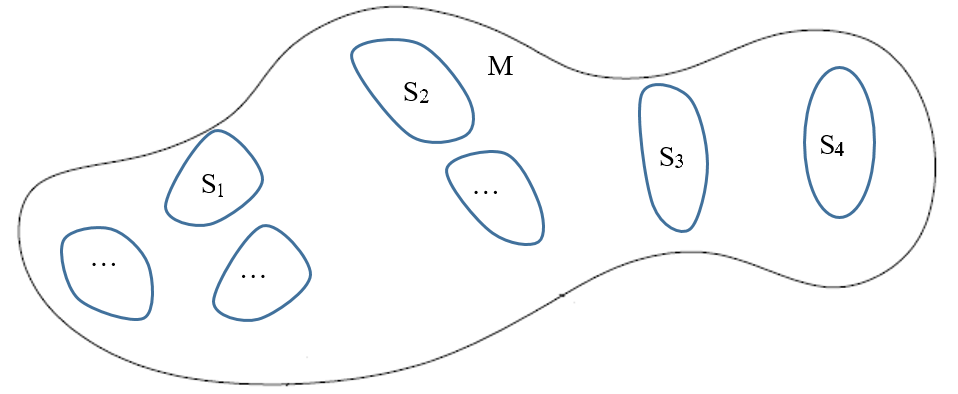
\includegraphics[width=0.7\linewidth]{source/MMD.png}
	\caption{流形的局部线性近似示意图}
	\label{fig:MMD}
\end{figure}\\
其中$M$表示的是原始的流形结构,文献\cite{Manifold_MMD}根据数据构建局部线性子空间$S_1,S_2,S_3,S_4,...$来近似表示流形$M$,然后通过点到点的距离定义点到子空间的距离再进一步定义子空间到子空间的距离,最后定义流形到流形的距离,从而进行图像集合的分类(下述定义中的$S,S_{i},C_{j}$表示的的是子空间而不是矩阵)。
\begin{itemize}
\item Point to point distance:$d_{ppd} (\bm{x},\bm{y})=\|\bm{x}-\bm{y}\|$
\item Point to subspace distance: $d_{psd} (\bm{x},S)=\min_{\bm{x}'\in S}\|\bm{x}-\bm{x}'\|$
\item Subspace to subspace distance: $d_{ssd} (S_1,S_2)= any~valid~subspace~metric$
\item Point to manifold distance: $d_{pmd} (\bm{x},M)=\min_{C_i\in M}d_{psd} (\bm{x},C_i )$
\item Subspace to manifold distance: $d_{smd} (S,M)=\min_{C_i\in M}d_{ssd} (S,C_i )$
\item Manifold to manifold distance: $d_{mmd} (M_1,M_2 )=\min_{C_i\in M_1}d_{smd} (C_i,M_2 )$
\end{itemize}
文章\cite{Manifold_MMD}利用上述的Manifold to manifold distance来度量流形之间的距离,然后在此距离上进行图像集合的分类问题,另一篇相关的工作\cite{Manifold_MDA}则是在\cite{Manifold_MMD}的基础上增加了判别信息得到了MDA(Manifold Discriminat Analysis)方法:在构建子空间$S_1,S_2,S_3,S_4,...$的时候要求类内散度尽量小而类间散度尽量大,如图\ref{fig:MDA}所示。
\begin{figure}[h]
	\centering
	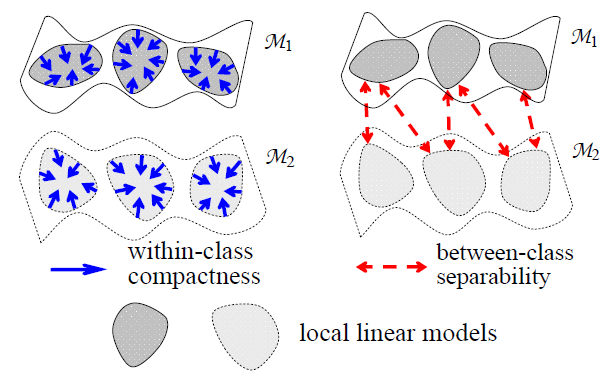
\includegraphics[width=0.7\linewidth]{source/MDA.png}
	\caption[MDA方法示意图]{MDA方法示意图(图片来自\cite{Manifold_MDA})}
	\label{fig:MDA}
\end{figure}

流形建模图像集合的方法是早期的流形学习的概念和图像集合问题的结合,在图像集合分类问题的研究上进行了有益的探索,也为后来的图像集合问题的研究(如\cite{Statistics_DARG,Statistics_BeyondGauss})提供了借鉴意义。
\subsection{仿射包建模的方法}
\label{sec:current_Affinehull}
仿射包建模的方法以其简单有效的特点在图像集合分类问题中被研究者所关注,该方法的代表作有\cite{Affinehull_AF,Affinehull_SANP,Affinehull_RNP,Affinehull_ProNN}。仿射包建模的图像集合的方法最核心的内容就是仿射包(Affine Hull)(由文献\cite{Affinehull_AF}引入到图像集合分类问题中),其定义如公式\ref{affinehull_samples}所示。
\begin{equation}
\label{affinehull_samples}
H_k=\left\{\bm{x}|\bm{x}=\sum_{i=1}^{n_{k}} \alpha_{ki} \bm{x}_{ki},\sum_{i=1}^{n_{k}} \alpha_{ki} =1 \right\}
\end{equation}
其中$k$是图像集合的下标,此外借助空间中的基向量(这里用$U_k$表示基矩阵)的概念还可以定义如下的形式:
\begin{equation}
\label{affinehull_bases}
H_k=\left\{\bm{x}|\bm{x}=\bm{\mu}_k+U_k \bm{v}_k,\bm{v}_k \in \mathbb{R}^l\right\} 
\end{equation}
两个仿射包之间的距离定义如公式\ref{affinehull_dist}所示。
\begin{equation}
\label{affinehull_dist}
D(H_1,H_2)=\min_{\bm{x}\in H_1}\min_{\bm{y}\in H_2}\|\bm{x}-\bm{y}\| 
\end{equation}
如果直接利用公式\ref{affinehull_dist}的定义进行图像集合分类的话容易出现两个仿射包相交(也就是距离为0)的情况。所以仿射包建模图像集合的一大问题就是对噪声不够鲁棒,针对这个问题,文献\cite{Affinehull_AF}中提出了使用Convex Hull的表示方法(如\ref{affinehull_convex}所示)。
\begin{equation}
\label{affinehull_convex}
H_k^c=\left\{\bm{x}|\bm{x}=\sum_{i=1}^n \alpha_{ki} \bm{x}_{ki},\sum_{i=1}^n \alpha_{ki}=1,L< \alpha_{ki}<U\right\} 
\end{equation}
来建模表示的方案,其中$L,U$分别表示上界和下界(标量),这样做的目的是将$\alpha_{ki}$限制在了一定的范围内来提高了模型对噪声的鲁棒性。

针对Affine Hull对样本不鲁棒的问题,\cite{Affinehull_SANP}提出了使用稀疏表示的方案来解决:
\begin{equation}
\left\{
\begin{split}
\label{affinehull_SANP}
F_{\bm{v}_i,\bm{v}_j}&=\|(\bm{\mu}_i+U_i \bm{v}_i)-(\bm{\mu}_j+U_j \bm{v}_j)\|_{2}^{2}\\
G_{\bm{v}_i,\bm{\alpha}}&=\|(\bm{\mu}_i+U_i \bm{v}_i)-X_i \bm{\alpha}\|_{2}^{2}\\
Q_{\bm{v}_j,\bm{\beta}}&=\|(\bm{\mu}_j+U_j \bm{v}_j)-X_j \bm{\beta}\|_{2}^{2}\\
\min_{\bm{v}_i,\bm{v}_j,\bm{\alpha},\bm{\beta}}&(F_{\bm{v}_i,\bm{v}_j}+\gamma(G_{\bm{v}_i,\alpha}+Q_{\bm{v}_j,\beta})+\lambda_1 \|\bm{\alpha}\|_1+\lambda_2 \|\bm{\beta}\|_1)
\end{split}
\right.
\end{equation}
这样做虽然使得模型对噪声更鲁棒,但是也带来计算复杂度太高的问题;所以\cite{Affinehull_RNP}提出了使用$l_p$范数(通常$p=2$)来代替$l_1$范数。
\begin{equation}
\label{affinehull_RNP}
\min_{\bm{\alpha},\bm{\beta}}\left(\|X\bm{\alpha}-Y\bm{\beta}\|_2^2+\lambda_1 \|\bm{\alpha}\|_{l_p}+\lambda_2 \|\bm{\beta}\|_{l_p}\right),s.t~\sum_{k}\alpha_k =1,\sum_k\beta_k =1
\end{equation}

而文章\cite{Affinehull_ProNN}则使用了高斯模型来增强模型的鲁棒性,使得在最小的误差情况下还要求样本属于该类的概率最大。

最后用图\ref{fig:Affinehull_relation}总结一下仿射包建模图像集合方法之间的关系。
\begin{figure}[h]
	\centering
	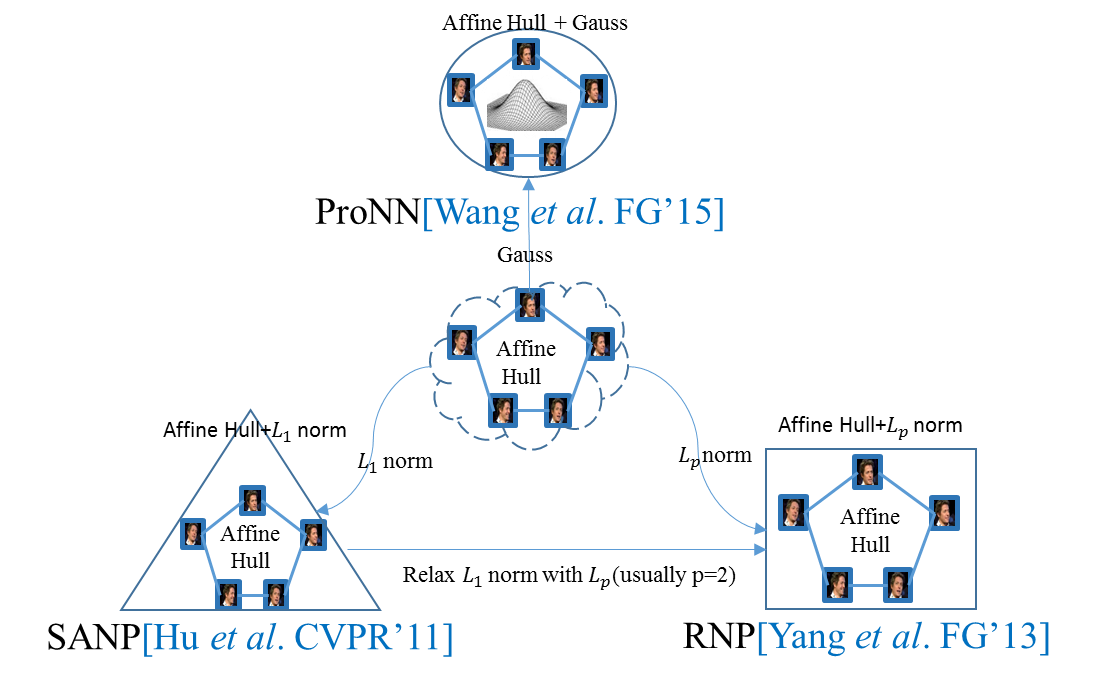
\includegraphics[width=0.7\linewidth]{source/Affinehull_relation.png}
	\caption{仿射包建模图像集合方法关系图}
	\label{fig:Affinehull_relation}
\end{figure}

概括起来就是:仿射包方法使用仿射包建模图像集合,为了克服直接使用仿射包分类对噪声不鲁棒问题,不同的限制被添加从而衍生出了不同的方法。
\subsection{统计建模图像集合的方法}
\label{sec:current_Statistics}
统计量建模的方法是近年来研究图像集合分类问题的主流方法之一,它以其优越的表现受到越来越多的关注。此外由于统计建模时,数据表示的特殊性(对称正定矩阵(SPD矩阵),分布函数等),黎曼流形成为了主要的研究工具。

统计建模的方法又可以细分为:单一统计量建模的方法,多统模型融合的方法以及基于分布函数的方法:
在单统计量表示图像集合的方法中,协方差矩阵被认为是丰富而有效的特征表示,样本协方差矩阵:$C=\frac{1}{n-1}\sum_{i=1}^n (\bm{x}_i-\bar{\bm{x}})$(其中$\bar{\bm{x}}=\frac{1}{n}\sum_{i=1}^n \bm{x}_i$为样本均值)一般是正定的$C \succ 0$,因此其并不构成空间,图\ref{fig:2d_SPD_cone}给出了2*2对称正定矩阵在三维空间中的例子\footnote{需要注意的是:$2\times 2$对称正定矩阵组成的集合本身并不包含这些外边界(因为它是开集),而是该边界包住的整个锥的内部}。
\begin{figure}[h]
	\centering
	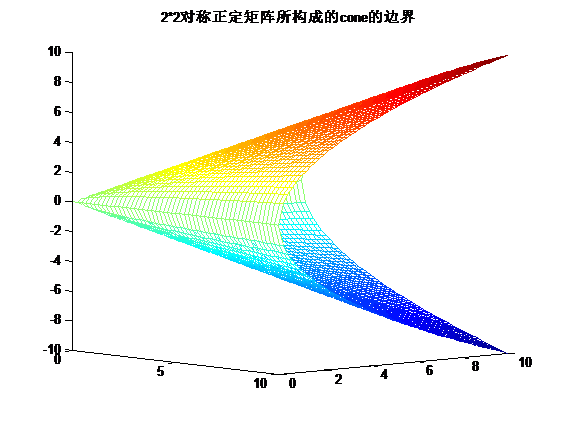
\includegraphics[width=0.5\linewidth]{source/2d_SPD_cone.png}
	\caption{$2\times 2$对称正定矩阵的外边界在3维空间中的结构}
	\label{fig:2d_SPD_cone}
\end{figure}

协方差建模图像集合的代表作\cite{Statistics_CDL}:利用核函数$\phi=\log(.)$将协方差矩阵流形映射到RKHS空间,在新的RKHS空间中,使用KPLS\cite{Kernel_KPLS}回归以及KDA\cite{Kernel_KDA}对视频人脸,多视角图像集等图像集合数据进行分类。

文献\cite{Statistics_SPDML}则在对称正定矩阵集合中,利用黎曼度量进行协方差降维及判别学习,算法的优化的空间(投影矩阵所在的空间)为Grassmann流形。

多统计模型融合的方法主要的代表作有\cite{Statistics_LMKML}和\cite{Statistics_HERML},两者的思想比较近似,主要思想是:不同的统计模型会刻画目标的不同侧面,包含了不同的信息,融合它们可以得到目标的更全面的表示。在具体实现过程中,工作\cite{Statistics_LMKML}首先利用核映射将不同统计模型映射到再生核希尔伯特空间(Reproducing Kernel Hilbert Space, RKHS)中,然后利用局部多核度量学习将其整合到一起进行分类,其算法流程如图\ref{fig:subfig_LMKML}所示。工作\cite{Statistics_HERML}首先也利用核函数将不同的统计模型映射到统一的再生核希尔伯特空间空间中,然后在新的再生核希尔伯特空间中利用融合的特征进行分类,其核心内容可以用图\ref{fig:Multi_Stat}描述。
\begin{figure}[h]
  \centering
  \subcaptionbox{LMKML\cite{Statistics_LMKML}方法流程图\label{fig:subfig_LMKML}(图片来自\cite{Statistics_LMKML})}
      {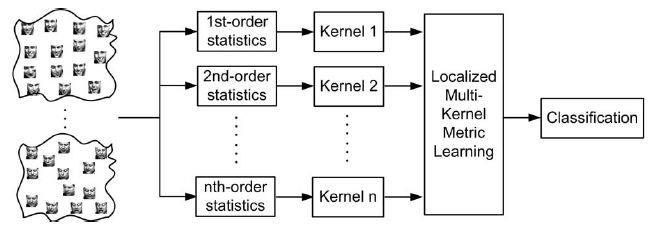
\includegraphics[width=0.51\linewidth]{source/Statistics_LMKML.png}}
  \hspace{1em}%
  \subcaptionbox{HERML\cite{Statistics_HERML}方法流程图\label{fig:subfig_HERML}(图片来自\cite{Statistics_HERML})}
      {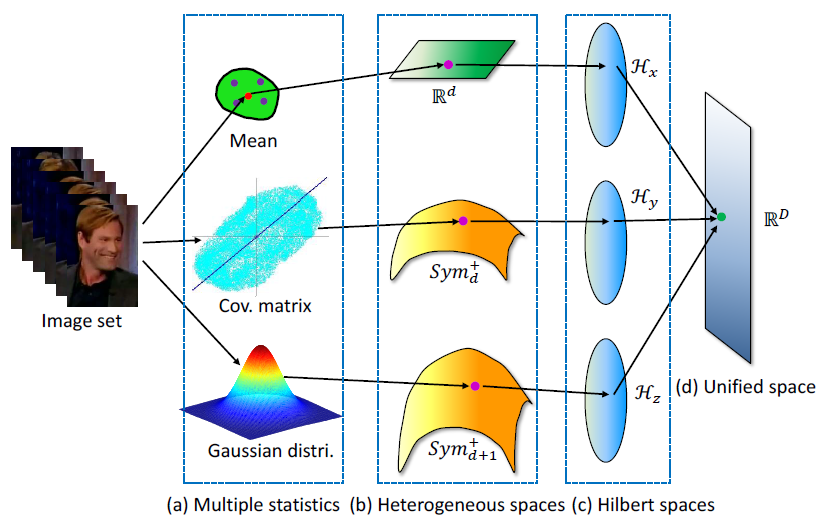
\includegraphics[width=0.45\linewidth]{source/Statistics_HERML.png}}
  \caption{多统计模型建模图像集合方法}
  \label{fig:Multi_Stat}
\end{figure}

为了更好的挖掘图像集合原始分布的信息,分布函数建模图像集合的方法被提出:文献\cite{Statistics_DARG}使用高斯混合模型(GMM)表示图像集合(逼近原始分布),利用核映射将GMM的各个component映射到RKHS中,并在核判别学习(Kernel Discriminant Analysis, KDA)\cite{Kernel_KDA}的框架下学习投影矩阵,最后在投影空间中分类;而文献\cite{Statistics_BeyondGauss}则使用KDE(Kernel Density Estimation)表示图像集合(逼近原始分布),并设计距离/散度来度量两个图像集合的KDE表示的距离,为了使得KDE估计可靠,文章中还为数据学习一个具有判别性的降维矩阵$W$来辅助估计。

统计建模图像集合的方法小结:1)统计建模的方法从最初的单统计量模型开始,经过发展逐步形成多统计模型融合以及分布函数建模图像集合等一系列方法;2) 由于数据表示的特殊性,统计模型的数学表示往往与黎曼流形相关联,黎曼流形成了研究它们的一个重要工具。图\ref{fig:Statistics_relation}描述了已有的统计建模图像集合的方法的一些关系。
\begin{figure}[h]
	\centering
	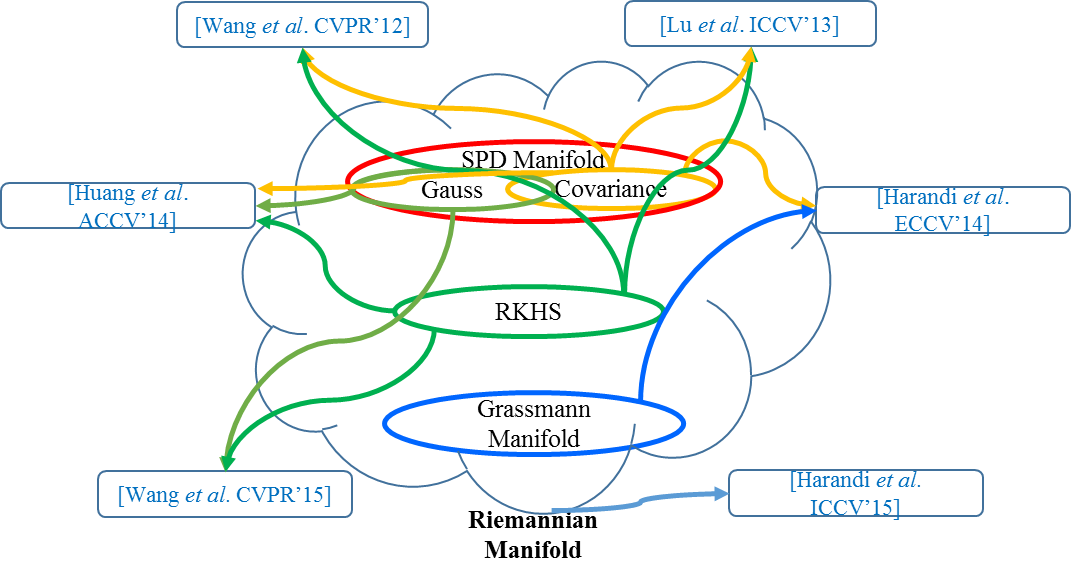
\includegraphics[width=0.7\linewidth]{source/Statistics_relation.png}
	\caption{统计建模图像集合的方法间的关系}
	\label{fig:Statistics_relation}
\end{figure}
\subsection{深度学习的方法}
\label{sec:current_Deeplearning}
深度学习在众多的领域都取得了不小的成果,所以也有学者将深度学习(Deep Learning, DL)的方法用于图像集合分类.目前这种尝试的主流做法是为每类学一个网络,并期望深度网络能够学到原始流形的geometry的结构。两个代表性的工作是:文献\cite{Deeplearning_DRM}为每类学一个AE-Like(Unsupervised)网络(网络结构如图\ref{fig:subfig_DRM}所示),自动挖掘Manifold的Geometry结构,最终利用重建误差以及投票进行分类。文献\cite{Deeplearning_MMDML}为每类学一个DNN-Like(Supervised)网络,使得在输出层不同类的margin尽量大;其网络结构如图\ref{fig:subfig_MMDML}所示。
\begin{figure}[h]
  \centering
  \subcaptionbox{DRMs-WV\cite{Deeplearning_DRM}方法网络结构\label{fig:subfig_DRM}(图片来源于\cite{Deeplearning_DRM})}
      {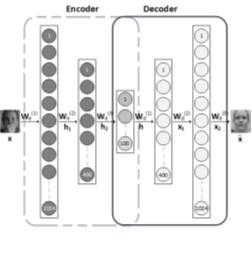
\includegraphics[width=0.3\linewidth]{source/Deeplearning_DRM.png}}
  \hspace{4em}%
  \subcaptionbox{MMDML\cite{Deeplearning_MMDML}方法流程图\label{fig:subfig_MMDML}(图片来自\cite{Deeplearning_MMDML})}
      {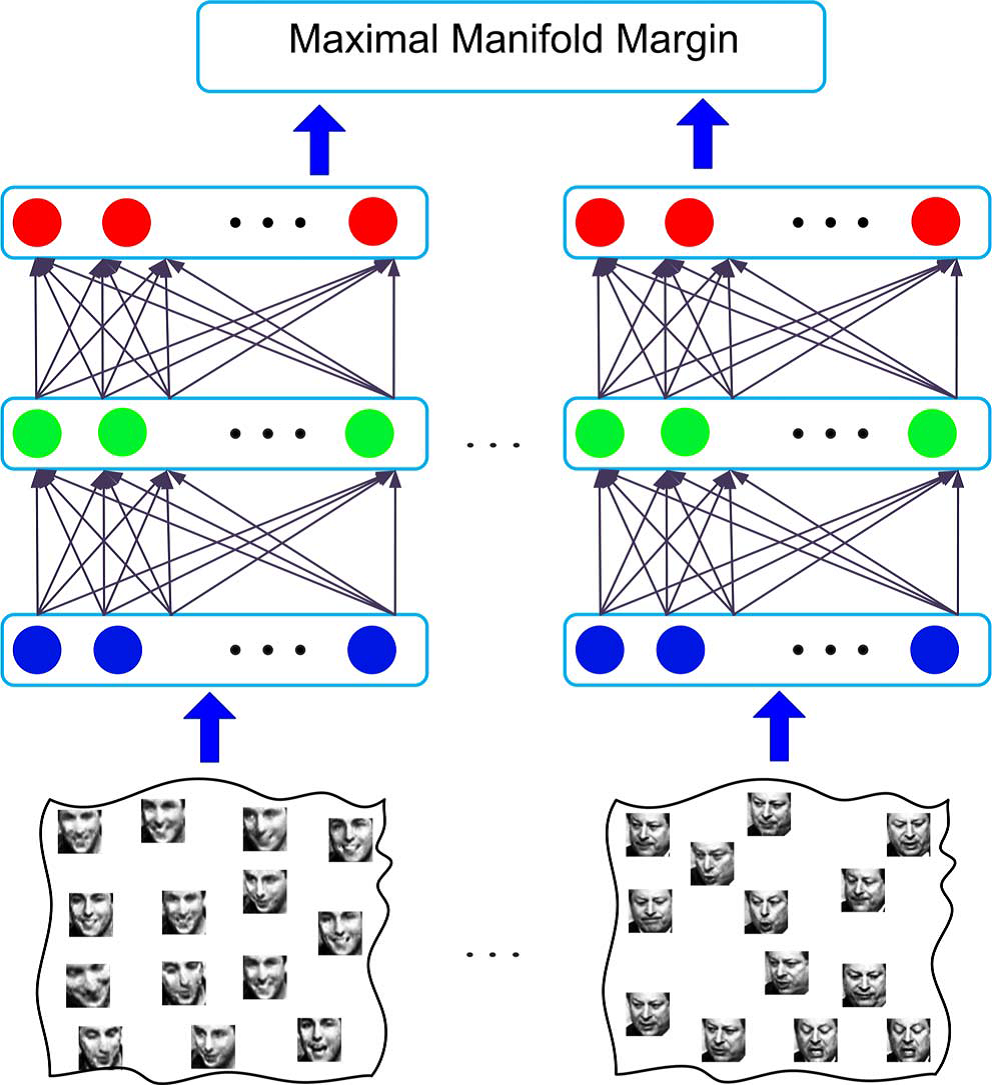
\includegraphics[width=0.3\linewidth]{source/Deeplearning_MMDML.png}}
  \caption{深度学习建模图像集合的代表性网络结构}
  \label{fig:Deepleaning_Nets}
\end{figure}

深度学习将计算机视觉的发展推向了一个新的高度,也为图像集合的研究注入了新的活力,所以这里使用一定的篇幅对其进行系统的介绍;由于工作\cite{Deeplearning_MMDML}是对工作\cite{Deeplearning_DRM}的改进,所以这里仅以MMDML\cite{Deeplearning_MMDML}为例对该类方法做一个介绍:在L+1层的DNN网络中,对于第$c$个图像集合的第$i$张图片其顶层输出如公式\ref{L_layer_output}所示。
\begin{equation}
\label{L_layer_output}
\bm{h}_{ci}^{L}=s(W_{c}^{L}\bm{h}_{ci}^{L-1}+\bm{b}_{c}^{L})
\end{equation}
其中$W_c^L$是投影矩阵,$\bm{b}_c^L$是偏置向量,$\bm{h}_{ci}^{L-1}$是上一层输出,$s(.)$为非线性激活函数;MMDML\cite{Deeplearning_MMDML}方法在网络顶层最大化不同manifold之间的margin;为此,工作\cite{Deeplearning_MMDML}为每类的每个样本(如第$c$类的第$i$个样本)定义公式\ref{MMDML_neighbor_descri}中的近邻关系描述。
\begin{equation}
\label{MMDML_neighbor_descri}
\left\{
\begin{split}
&D_1 (\bm{h}_{ci}^L )=\frac{1}{K_1}\sum_{p=1}^{K_1}\|\bm{h}_{ci}^{L}-\bm{h}_{cip}^L\|_2^2\\
&D_2 (\bm{h}_{ci}^L )=\frac{1}{K_2}\sum_{q=1}^{K_2}\|\bm{h}_{ci}^L-\bm{h}_{ciq}^L\|_2^2 
\end{split}
\right.
\end{equation}
其中$\bm{h}_{cip}^L$表示的是当前样本的第$p$个同类近邻在网络顶层的输出,$\bm{h}_{ciq}^L$表示的是当前样本的第$q$个不同类的近邻在网络顶层的输出,$K_1,K_2$是两个设置近邻个数的参数。故上式定义了第$c$类的第$i$个样本在网络顶层与$K_1$个同类近邻,$K_2$个不同类近邻的关系。

MMDML方法的目标是在网络顶层最大化不同manifold之间的margin:

首先使用$f_c=[W_c^1,W_c^2,\cdots,W_c^L,\bm{b}_c^1,\bm{b}_c^2,\cdots,\bm{b}_c^L]$表示网络参数,然后定义:
\begin{equation}
\label{Layer_Loss}
\left\{
\begin{split}
&H_1=\sum_{c=1}^C\sum_{i=1}^{N_c}g(D_1(\bm{h}_{ci}^{L})-D_2(\bm{h}_{ci}^L))\\
&H_2=\sum_{c=1}^C\sum_{l=1}^L(\|W_{c}^{l}\|_{F}^{2}+\|\bm{b}_{c}^{l}\|_{2}^2)
\end{split}
\right.
\end{equation}

其中$g(a)=\frac{1}{\rho}\log(1+\exp(\rho a))$($\rho$表示锐度参数),$N_c$表示第$c$个图像集合中的样本数。利用公式\ref{Layer_Loss}得到MMDL的优化目标:
\begin{displaymath}
\min_{f_1,f_2,\cdots,f_C }H= H_1+\frac{1}{2}H_2
\end{displaymath}

文献\cite{Deeplearning_MMDML}中使用了随机次梯度下降算法训练网络参数,在最后在测试阶段,测试样本的分类结果由公式\ref{MMDML_classify}获得。
\begin{equation}
\label{MMDML_classify}
L_q=\arg\min_c d(X_q,X_c),1\leq c\leq C
\end{equation}
其中$X_q=[\bm{x}_1^q,\bm{x}_2^q,\cdots,\bm{x}_{N_q}^q]$表示的是一个测试图像集$X_c$表示的是一个训练图像集,而$d(X_q,X_c)$的计算过程如下:1)使用第$c$个网络将$\bm{x}_j^q$映射到新的空间$\bm{h}_c (\bm{x}_j^q )$;2)计算$\bm{h}_c (\bm{x}_j^q )$与$\bm{h}_{ci}^L,i=1,2,\cdots,N_c$的欧氏距离,并将最小的距离作为$\bm{x}_j^q$与第$c$个manifold的距离,最后对所有样本$\bm{x}_1^q,\bm{x}_2^q,\cdots,\bm{x}_{N_q}^q$求平均作为$d(X_q,X_c)$。
\subsection{国内外研究现状小结}
\label{sec:current_Summarize}
总结国内外对图像集合分类问题的研究,对图像集合分类问题的研究可做如下描述:1)为图像集合设计一种表示(子空间、流形、仿射包、统计模型及深度网络等);2)为这种表示(模型)设计/定义一种距离度量,并用距离/度量进行判别学习;3)(可选)针对已有模型问题(不鲁棒、维度太高……)做进一步改进。

另一方面,在图像集合分类问题中,由于数据的特殊性,往往需要对非线性的数据模型进行研究,如:子空间、统计模型等。在这些模型的研究中,黎曼流形作为成熟的数学工具在其中发挥了重要的作用。 

最后,还需要注意到除了前面介绍的一些方法,还有其它一些方法,如:稀疏编码和协同表示的方法也为图像集合的分类问题的探索做出了重要贡献。
\section{数据介绍}
\label{sec:data_intro}
图像集合分类问题源于实际,最终还是要回到实际中;所以只有理论还是不够,还需要数据的支撑。本小节就是对图像集合分类问题中的一些常用的数据集进行介绍;此外,多样化的数据也更能说明算法的有效性,并且本文对黎曼流形问题的研究过程中并没有限制在图像集合问题上,所以这里还会介绍一个可用黎曼流形建模的数据集合,表格\ref{tab:database_list}中列出了本节将要介绍的数据库。
\begin{table}[htb]
	\centering
	\caption{数据库列表}
	\begin{tabular}{l|l|c}
	\toprule[1.5pt]
		{\heiti 数据库} &{\heiti 描述} &{\heiti 备注} \\ \hline
		YouTube Faces DB\cite{Database_YTF} &1595个人,3425段视频,低分辨高压缩率 &人脸数据库 \\ \hline
		YouTube Celebrity\cite{Database_YTC} &47个人,1910段视频, 低分辨高压缩率 &人脸数据库 \\ \hline
		UIUC\cite{Database_UIUC} &4个大类,18个子类,每类12张图片 &材质分类数据库 \\ \hline
		ETH-80\cite{Database_ETH80}   &共8个子类每类4个图像集合每个集合41张图片 &物体识别数据库 \\ \hline
		CMU MoBo\cite{Database_MoBo} &25个人,4个运动(行走)类,150段视频数据 &为步态研究而搜集 \\
	\bottomrule[1.5pt]
	\end{tabular}
	\label{tab:database_list}
\end{table}
图\ref{fig:databases_exmples}给出这些数据集的一些示例图片。
\begin{figure}[htb]
	\centering
	\subcaptionbox{YouTube Faces DB\cite{Database_YTF}数据库示例\label{fig:subfig_database_YTF}}
      	{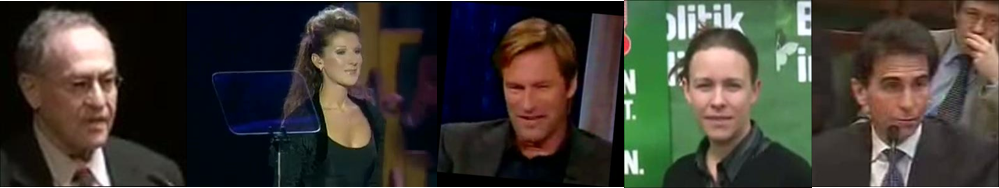
\includegraphics[width=0.49\linewidth]{source/YTF.png}}
  	\subcaptionbox{YouTube Celebrity\cite{Database_YTC}数据库实例\label{fig:subfig_database_YTC}}
      	{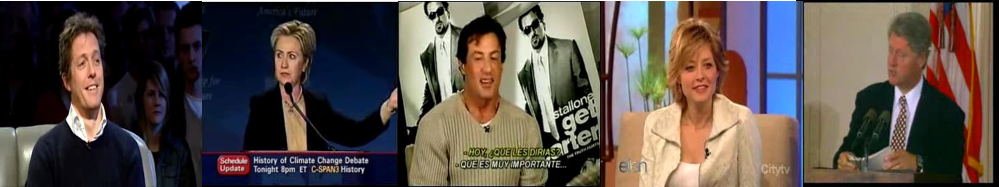
\includegraphics[width=0.49\linewidth]{source/YTC.png}}
  	\subcaptionbox{UIUC\cite{Database_UIUC}数据库示例\label{fig:subfig_database_UIUC}}
    	{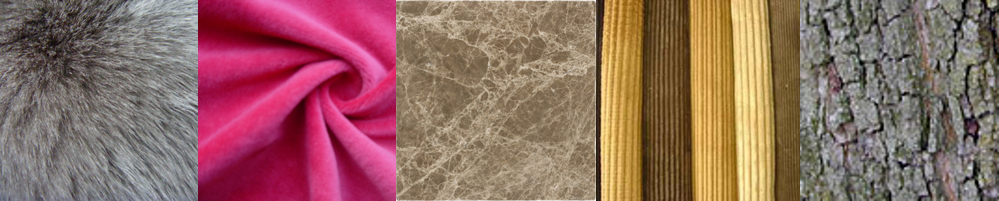
\includegraphics[width=0.49\linewidth]{source/UIUC.png}}
    \subcaptionbox{ETH80\cite{Database_ETH80}数据库示例\label{fig:subfig_database_ETH80}}
      	{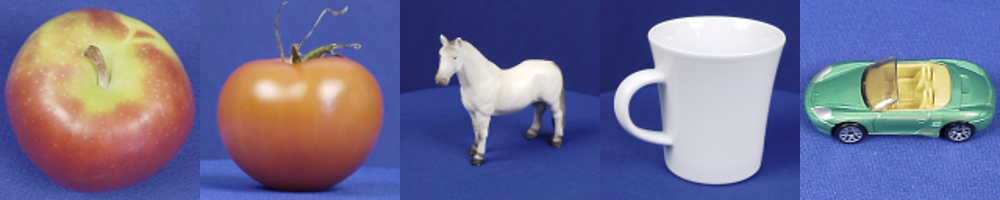
\includegraphics[width=0.49\linewidth]{source/ETH80.png}}
    \subcaptionbox{CMU MoBo\cite{Database_MoBo}数据库示例\label{fig:subfig_database_CMU_MoBo}}
      	{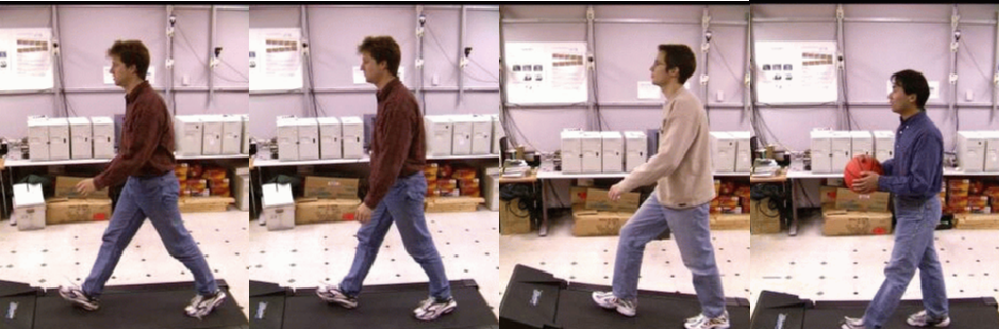
\includegraphics[width=0.5\linewidth]{source/CMUMoBo.png}}
  	\caption{数据库示例}
  	\label{fig:databases_exmples}
\end{figure}

YouTube Faces DB数据库\cite{Database_YTF}最初是为视频人脸验证任务收集的,其收集过程中根据LFW(Labeled Faces in the Wild\cite{Database_LFW})数据集的样本进行,数据库包含了1595个人的3425个视频段,是一个较大的视频数据库,这些数据均从Youtube上获得,最短的只有48帧,最长的则有6070帧;由于数据是从网络中收集的所以存在脸部姿态变化,表情变化等一系列问题。

Youtube Celebrity数据集\cite{Database_YTC}也是从YouTube上收集而来,最初是为人脸跟踪和识别任务而收集的,数据集包含47个人的1910个视频段,属于是较大的一个视频数据库。其数据呈现出低分辨率和高压缩率的特点,此外同样存在脸部姿态变化、表情变化等问题。数据库的状况比较接近于真实情况,识别任务有不小的挑战。

UIUC数据库\cite{Database_UIUC}是材质数据库(material database),数据库的组织结构大致为:顶层是四个大类,分别是树皮、织物、建筑材料和动物的皮毛,下面分出18个子类,每个子类包含了12张图像,该数据集并不属于图像集合的数据集,但是当使用Region Covariance为图像建模表示的时候,该数据集上的分类问题研究也将与SPD矩阵黎曼流形相关。

ETH80数据库\cite{Database_ETH80}主要用于物体识别任务,数据集中的数据从概念上属于4个大类:水果蔬菜类、动物类、(小型的)人造的类别及(大型的)人造的类别,具体采集了8个类别:苹果、牛、杯子、狗、马、梨、西红柿、和汽车,整个数据集包含80个图像集合(每个类别10个集合),每个集合包含41张图片,所以数据集总大小为3280张图片。

CMU MoBo数据库\cite{Database_MoBo}包含25个人在室内环境下,跑步机上的6个view行走姿态的150段视频数据,数据库中的数据主要有4种行走姿态(摄像机帧率30FPS):慢速行走,快速行走,斜面行走以及带球行走。

在本节的最后简单的介绍一下测试协议的问题,其中由于CMU MoBo\cite{Database_MoBo}提出的时间相对比较早,所以这里不再介绍它的测试协议,此外该数据集也不会在实际的实验中使用。而YouTube Faces DB数据库由于做的是人脸验证任务,与分类识别任务有所区别,在本文的实际实验中也没有列入,但是考虑到今后可能会用到这个数据库(毕竟它是相当大的视频人脸数据库)所以这里仍然简单介绍一下它的测试协议。

在所有的数据集上均采用了10折交叉验证,最后报告的结果均是10则交叉验证的平均结果,其中在每一次验证过程中我们将训练集称为Gallery测试集称为Probe,在各个数据集合上对数的划分情况如下:在YTF(YouTube Faces DB)上根据文献\cite{Database_YTF}中的方式,将数据库提供的5000对视频对平均分为10份(每份500对,其中250对的每对是同一个人,另外250对的每对不是同一个人)。在YTC(YouTube Celebrity)\cite{Database_YTC}上数据的划分则是参考了\cite{Statistics_CDL}以及\cite{Statistics_Vemu}的数据划分方式,在YTC数据集合上对每个人随机选取3个视频段作为训练(Gallery)6个视频段作为测试(Probe),然后将这个过程重复进行10次来获得数据集的随机划分。在UIUC数据库\cite{Database_UIUC}上的数据划分比较简单,我们随机从每个子类中选取一半的样本做为训练集(Gallery)剩下的一半的数据作为测试集(Probe),然后也重复这个过程10次得到10次验证的数据。ETH80数据上的数据划分也参考了\cite{Statistics_CDL},其上的数据划分是在每个类别中随机选取5个图像集合作为训练集(Gallery)剩下的5个作为测试集(Probe),并重复这个过程10次作为10次验证的数据。以上便是本文中使用的数据库的数据划分方式和测试协议。
\section{本文的组织结构}
\label{sec:struct}
在本章的最后,我们来介绍一下本文的组织结构:第一章是绪论,这一章主要介绍问题的背景意义以及国内外的研究现状。作为本文的第一章主要目的是引领读者对图像集合分类问题有一个宏观的了解,也为后续自己工作的介绍做准备。

第二章将介绍矩阵函数与黎曼流形上的优化问题,这部分的内容通过对黎曼流形,矩阵函数等基本概念的介绍,对矩阵函数求导和流形优化等一般化的问题进行了初步的探究。并结合本文其它两个研究内容中的一些实际问题对其进行展开,目的是方便读者理解和实现本文中的提到的方法和概念的同时帮助读者在遇到类似问题的时候能够从中获得启示。

第三章介绍黎曼流形上的偏最小二乘问题,这一章的内容会从欧氏空间的偏最小二乘问题开始介绍,然后借助投影的一般形式将其扩展到黎曼流形中得到黎曼流形上偏最小二乘问题的基础版本的,紧接着是结合流形的特点以及考虑到数据的稀疏性问题,从基础版本的黎曼流形上的偏最小二乘方法出发提出了多切空间逐步回归的偏最小二乘学习方法,最后实验验证了该方法。

第三章简单回顾了使用子空间和协方差矩阵表示图像集合的方法的问题后,考虑使用半正定(PSD)矩阵表示图像集合,在对早期工作以及工作\cite{PSD_WACV}中的不足进行分析之后,提出了使用嵌入判别信息的低秩对称半正定矩阵建模图像集合的方法,最终实验验证了该建模方法的有效性。

第五章总结和讨论前几章的内容,对现有研究做了回顾与不足之处的分析,并对下一步可能的方向做了讨论和展望。
% created on 2016-03-27
\chapter{矩阵函数的导数计算与矩阵流形上的基本优化方法}
\label{chap:Matdev_basicManiopt}
《论语》有云:“工欲善其事,必先利其器”。本文把黎曼流形作为主要的研究工具/对象,则必然涉及到其上的优化问题,本章正是对该问题的探索。不过本章的内容也是一个一般化的问题研究而并不仅限于本文中的应用,最后这部分内容也是对研究课题中流形上的优化问题的归纳和总结。当然这里不会像\cite{Maniopt_DiscreteCurveFitting}或\cite{Maniopt_book}中那样详细的介绍黎曼流形上的优化问题。作为基础这里首先会介绍黎曼流形这个基础的概念,然后探究矩阵函数和它们的导数计算与优化问题,最后结合学位论文课题中提炼出的相关实例对矩阵流形优化进行介绍。目的一是方便读者理解作者学位论文中研究课题,目的二是为了让读者在遇到类似问题的时候能够从中提炼出思路或解决方案。

对于流形上很细节的问题读者还是到文献\cite{Maniopt_DiscreteCurveFitting,Maniopt_book}中寻找答案会更合适。此外,本章的内容不会对算法的收敛性等专业的问题作讨论,因为这既非作者所长也不是这里的写作目的,并且这可能会让内容过于专业化而变得枯燥乏味。
\section{黎曼流形简介}
\label{sec:manifold}
黎曼流形作为本工作的主要研究对象之一,将在这一节对其进行简要介绍。本节的内容主要包括两部分:第一部分是基本流形和黎曼流形的基本定义和性质的介绍;第二部分将就黎曼流形中的对称正定矩阵流形(Symmetric Positive Define, SPD)矩阵流形做进一步的介绍,并着重介绍SPD流形上的两个重要的度量(Affine Invariant Metric, AIM和Log-Euclidean Metric, LEM)(本节的一些内容尤其是一些流形上的基本定义的介绍参考了\cite{Manifold}和\cite{PHDThesis})。
\subsection{黎曼流形}
\label{sec:manifold_Riemaniann}
流形是数学上抽象概念,它的定义则依赖另一个更抽象的概念——拓扑空间:
\begin{definition}
\label{Topology}
{\heiti(拓扑空间)} 设$S$表示一个集合,$\tau$也是一个集合且$\tau$中的元素满足:
\begin{enumerate}
\item $\varnothing,S \in \tau$;
\item $\tau$中有限个元素的交仍然属于$\tau$
\item $\tau$中任意多个元素的并仍然属于$\tau$
\end{enumerate}
\end{definition}

在数学上,这样的$\tau$称为$S$上的拓扑结构,并且将$\tau$中的元素叫作开集;拓扑的研究中,点集拓扑是一个重要的内容。关于点集拓扑两个概念需要理解(系统的内容可以参看\cite{Manifold}),第一个概念(空间是$A_2$的):如果一个拓扑空间具有可数拓扑基则这样的拓扑空间\footnote{具有这样性质的空间也叫做{\heiti 第二可数的}}称为$A_2$的;第二个概念(空间是$T_2$的):如果一个拓扑空间具有Hausdorff性质则这样的的拓扑空间称为$T_2$的。Hausdorff性质:假设$S$是拓扑空间,设$\bm{x}$和$\bm{y}$是$S$中的点,我们称$\bm{x}$和$\bm{y}$可以“由邻域分离”,如果存在$\bm{x}$的邻域$U$和$\bm{y}$的邻域$V$使得$U$和$V$是不相交的(即:$U \cap V = \varnothing$),且任何两个$S$中不同的点都可以有这样的邻域分离,那么称$\bm{X}$是豪斯多夫(Hausdorff)空间,因此豪斯多夫空间又叫做分离空间。$A_2,T_2$这两个基本的概念在本文的研究中不会涉及,此处是出于完备性的考虑将其放在这里。
\begin{definition}
\label{C_r_Continuous}
{\heiti($r$阶连续)}若一函数是连续的,则属于$C^0$函数。若函数存在连续导函数,则属于$C^1$函数;若函数$r$阶可导,并且其$r$阶导函数连续,则属于$C^r$函数($r \geq 1$)。而任意光滑函数是对所有$r$都有$r$阶的连续导数,并用$C^\infty$表示这一类函数。
\end{definition}
\begin{definition}
\label{Homeomorphism}
{\heiti(同胚)}两个拓扑空间$\{X,\tau_X\}$和$\{Y,\tau_Y\}$之间的函数$f:X \rightarrow Y$称为同胚,如果它具有下列性质:
\begin{enumerate}
\item $f$是双射(单射和满射)
\item $f$是连续的
\item 反函数$f^{-1}$也是连续的($f$是开映射)
\end{enumerate}
\end{definition}
关于同胚,此处定义参考维基百科\footnote{\url{https://zh.wikipedia.org/wiki/\%E5\%90\%8C\%E8\%83\%9A}}以及文献\cite{Manifold}。
\begin{definition}
\label{C_r_Manifold}
{\heiti($\bm{C^r}$流形)}设$M$是具有$A_2,T_2$性质的拓扑空间,如果存在$M$的开覆盖$\{U_\alpha\},{\alpha \in \Gamma}$以及相应的连续映射族$\varphi_\alpha:U_\alpha \rightarrow \varphi_\alpha(U_\alpha)$;使得:
\begin{enumerate}
\item $\varphi_\alpha:U_\alpha \rightarrow \varphi_\alpha(U_\alpha) \subset \mathbb{R}^{n}$为从$U_\alpha$到欧氏空间开集$\varphi_\alpha(U_\alpha)$上的同胚\footnote{这里的$n$称为流形$M$的维度,记为${\rm dim}(M)=n$}
\item 当$U_\alpha \cap U_\beta \neq \varnothing$时,若如下的转换映射:
\begin{displaymath}
\varphi_{\beta} \circ \varphi_{\alpha}^{-1}:\varphi_\alpha(U_\alpha \cap U_\beta) \rightarrow \varphi_\beta(U_\alpha \cap U_\beta)
\end{displaymath}
\end{enumerate}
属于$C^r(r\geq 1)$映射,则称$M$为$C^r$流形。
\end{definition}
特别地,若$r=0$则称$M$为拓扑流形,又若$r\geq 1$则称$M$为$C^r$微分流形,进一步令$\mathcal{D}=\{(U_{\alpha},\varphi_\alpha),\alpha \in \Gamma\}$;若$\mathcal{D}$是最大的,也就是说当坐标卡$(U,\varphi)$与$\mathcal{D}$中任意的$(U_{\alpha},\varphi_\alpha)$都是$C^r$相容\footnote{设$U$为$M$上的开集,$\varphi:U \rightarrow \mathbb{R}^{n}$为连续映射,且$\varphi$的像为开集,$\varphi$到其像上是同胚。 如果$\varphi$和$\varphi_\alpha$之间的转换映射均为$C^r$的,则称$(U,\varphi)$和局部坐标覆盖$(U_\alpha, \varphi_{\alpha})$是$C^r$相容的(摘自\cite{Manifold})}的,则有$(U,\varphi)$属于$\mathcal{D}$,这样的$\mathcal{D}$称为拓扑流形$M$的一个$C^r$微分构造或微分结构(该部分总结自参考文献\cite{Manifold}第一章的定义1.1.1)。
\begin{definition}[a]
\label{Tangent_Vector_a}
{\heiti(切向量与切空间)}记$C^\infty(M)$为微分流形$M$上任意光滑函数的全体组成的向量空间。 设$p \in M$, 如果线性映射$X_p : C^\infty(M) \rightarrow \mathbb{R}$满足以下条件:
\begin{displaymath}
X_p(f\circ g) = X_p(g)f(p)+g(p)X_p(f),\forall f,g \in C^\infty(M)
\end{displaymath}
则称$X_p$为$p$处的切向量。切向量的全体组成的向量空间记为$p$处的切空间$T_pM$。
\end{definition}
上述定义的切向量比较比较晦涩,下面是关于切向量的另一个更加直观的定义形式:
\addtocounter{definition}{-1}
\begin{definition}[b]
\label{Tangent_Vector_b}
{\heiti(切向量)}
设$p\in M$,是流形$M$上的一点,经过$p$的光滑曲线$\sigma: (-a,a) \rightarrow  M$, 使得$\sigma(0)=p$,现定义$\sigma^{\prime}(0)$:
\begin{displaymath}
\sigma^{\prime}(0)f=\frac{d}{dt}|_{t=0}[f\circ\sigma(t)],\forall f \in C^\infty(M).
\end{displaymath}
容易验证$\sigma^{\prime}(0)\in T_pM$, 称为$\sigma$的初始切向量, 也记为$\dot{\sigma}(0)$。
\end{definition}
\begin{definition}
{\heiti(黎曼流形)}对任意$p\in M$, 如果映射$g_p : T_pM \times T_pM \rightarrow \mathbb{R}$满足条件:
\begin{enumerate}
\item $\forall \bm{x}_p \in T_p M,g_p(\bm{x}_p,\bm{x}_p)\geq 0$,等号成立当且仅当$\bm{x}_p=0$
\item $\forall \bm{x}_p,\bm{y}_p \in T_p M$,均有$g_p(\bm{x}_p,\bm{y}_p)=g_p(\bm{y}_p,\bm{x}_p)$
\end{enumerate}
则称$g$为$M$上的黎曼度量,$(M,g)$称为黎曼流形。
\end{definition}
\begin{definition}
{\heiti(曲线长度与距离)}沿用前面的定义,设$\sigma(t):[a,b]\rightarrow  M$表示黎曼流形$(M,g)$上的一条链接$p,q$的$C^{1}$曲线,其中自变量$t \in [a,b]$;定义曲线$\sigma$的长度为:
\begin{equation}
\label{Length}
L(\sigma)=\int_{a}^{b}{\|\dot{\sigma}(t)\|}dt
\end{equation}
\end{definition}
其中$\dot{\sigma}(t)$与定义\ref{Tangent_Vector_b}中的意义相同且$\|\dot{\sigma}(t)\|=g(\dot{\sigma}(t),\dot{\sigma}(t))^{1/2}$;最后利用公式\ref{Length}定义距离如公式\ref{Distance}所示。
\begin{equation}
\label{Distance}
d(p,q)=\inf_{\sigma}L(\sigma)
\end{equation}
最后,这里记录另一条对于计算距离有用的性质:在等距同构的映射下,新空间中测地线仍然是原来空间中的测地线的长度。
\subsection{对称正定矩阵流形}
\label{sec:Manifold_SPD}
对称正定矩阵流形是本文研究的主要对象之一,在前面的\ref{sec:current_Statistics}小节也有提到:统计建模图像集合的时候,其最终的数学形式往往以对称正定(Symmetric Positive Definite, PSD)矩阵的形式存在。而已经有充分的数学理论支撑,SPD矩阵空间在适合的度量定义下构成黎曼流形,其中最有名也最常用的是AIM\cite{AIM_metric}(Affine-Invariant Metric)和LEM\cite{LEM_metric}(Log-Euclidean metric)。下面首先给出对称正定矩阵的定义。
\begin{definition}
{\heiti(对称正定矩阵集合)} 由$d \times d$的对称正定矩阵构成的集合
\begin{equation}
\label{SPD_Matrices}
\mathbb{S}_{d}^{+}=\left\{A|A \in \mathbb{R}^{d\times d},\bm{x}^{T}A\bm{x} \geq 0,\forall \bm{x} \in \mathbb{R}^{d}~{\rm and}~\bm{x}^{T}A\bm{x}=0~{\rm iif}~\bm{x}=\bm{0}\right\}
\end{equation}
\end{definition}
当赋上适当的度量$g$(如AIM\cite{AIM_metric}或LEM\cite{LEM_metric})之后即构成黎曼流形$(\mathbb{S}_{d}^{+},g)$。

在PSD矩阵流形上,AIM度量\cite{AIM_metric}和LEM度量\cite{LEM_metric}各自的对数${\rm Log}$和指数${\rm Exp}$函数及距离分别由公式\ref{AIM}和\ref{LEM}描述。
\begin{equation}
\label{AIM}
\begin{split}
AIM:\left\{
\begin{aligned}
&\exp_{X_1}(H)=X_{1}^{\frac{1}{2}}\exp(X_{1}^{-\frac{1}{2}}HX_{1}^{-\frac{1}{2}})X_{1}^{\frac{1}{2}}\\
&\log_{{X_1}}({X_2})={X_{1}^{\frac{1}{2}}}\log({X_{1}^{-\frac{1}{2}}}{X_2}{X_{1}^{-\frac{1}{2}}}){X_{1}^{\frac{1}{2}}}\\
&\delta_{A}({X_1,X_2})=\left<\log_{{X_1}}({X_2}),\log_{{X_1}}({X_2})\right>_{{X_1}}\\
&~~~~~~~~~~~~~~~~=\|\log({X_{1}^{-\frac{1}{2}}}{X_2}{X_{1}^{-\frac{1}{2}}})\|_F
\end{aligned}
\right.
\end{split}
\end{equation}
其中${H}$是${X_1}$处的切空间上的切向量,$\left<\cdot,\cdot\right>_{{X_1}}$表示$X_1$的切空间上的黎曼度量(内积)
\begin{equation}
\label{LEM}
\begin{split}
LEM:\left\{
\begin{aligned}
&\exp_{{X_1}}({T_2})=\exp(\log({X_{1})}+D_{X_1}\log.({T_2}))\\
&\log_{{X_1}}({X_2})=D_{\log({X_1})}\exp.(\log({X_2})-\log({X_2}))\\
&\delta_{l}({X_1,X_2})=\left<\log_{{X_1}}({X_2}),\log_{{X_1}}({X_2})\right>_{{X_1}}\\
&~~~~~~~~~~~~~~~=\|\log({X_{1}})-\log({X_{2}})\|_F
\end{aligned}
\right.
\end{split}
\end{equation}
其中${T_2}$是${X_1}$处的切空间上的切向量,$D_{X_1}\log.(T_2)$表示的是$\log(X_1)$沿着方向$T_2$的方向导数,$\left<\cdot,\cdot\right>_{{X_1}}$表示的是$X_1$的切空间上的黎曼度量,$D_{\log({X})}\exp.=(D_{{X}}\log.)^{-1}$是由等式$\log \circ \exp={I}$,更多详细信息可参看文献\cite{LEM_metric}。
\section{优化问题与梯度}
\label{sec:opt_and_gradient}
本节会从一般的优化问题开始,以梯度相关的问题结束。第一部分是优化问题的介绍;由于优化问题多种多样,这里选取具有代表性的一类问题——Lagrange对偶问题进行介绍,接着第二部分会以梯度为主线介绍梯度在优化问题中应用,最后简要介绍梯度下降与共轭梯度算法,为将算法扩展到流形上做准备。
\subsection{拉格朗日对偶问题}
\label{sec:Lagrange_prob}
拉格朗日对偶问题(Lagrange Dual Problem)的转化是求解带约束问题重要方法,在带约束的优化问题中有着重要的地位,其转化过程将在接下来的部分进行描述,首先,假设有如下形式的原问题:
\begin{equation}
\label{Original_Prob}
\begin{split}
&\min f_0(\bm{x})\\
&s.t~~f_i(\bm{x})\leq 0,i=1,2,...,m\\
&~~~~~h_i(\bm{x}) =0,i=1,2,...,p\\
\end{split}
\end{equation}
对于原问题\ref{Original_Prob},其对应的Lagrange函数定义如式\ref{Lagrange_Func}所示。
\begin{equation}
\label{Lagrange_Func}
\mathcal{L}(\bm{x},\bm{\lambda},\bm{v})=f_0(\bm{x})+\sum_{i=1}^{m}\lambda_i f_i(\bm{x})+\sum_{i=1}^{p}v_ih_i(\bm{x})
\end{equation}
由Lagrange函数\ref{Lagrange_Func}定义原问题的Lagrange对偶函数\footnote{Lagrange对偶函数是一族仿射函数的下确界,所以它是凹函数,具体细节请参看《Convex optimization》}如式\ref{Lagrange_Dual}所示。
\begin{equation}
\label{Lagrange_Dual}
g(\bm{\lambda},\bm{v})=\inf_{x}\mathcal{L}(\bm{x},\bm{\lambda},\bm{v})=\inf_{x}\left(f_0(\bm{x})+\sum_{i=1}^{m}\lambda_i f_i(\bm{x})+\sum_{i=1}^{p}v_ih_i(\bm{x})\right)
\end{equation}
其中$\inf$是下确界的意思,其意义类似于最小值,但是稍有不同的是:例如对于开区间$(0,1)$它的最小值是不存在的,但是它的下确界却是存在的$0=\inf\{(0,1)\}$。关于对偶问题\ref{Lagrange_Dual}需要了解的是:对偶问题\ref{Lagrange_Dual}对任意的$\bm{\lambda} \geq \bm{0}$以及$\bm{v}$都是原问题\ref{Original_Prob}的下界,此外对于$\bm{\lambda} < \bm{0}$的情形这将导致$g(\bm{\lambda},\bm{v})$失去实际意义。

既然$(\bm{\lambda},\bm{v})$对于任意的$\bm{\lambda} \geq \bm{0}$以及$\bm{v}$是原问题\ref{Original_Prob}的下界,那么什么样的$\bm{\lambda},\bm{v}$才是好的?对偶问题考虑:
\begin{equation}
\label{Dual_Prob}
\max g(\bm{\lambda},\bm{v}),s.t~\bm{\lambda} \geq \bm{0}
\end{equation}
所以实际上的Lagrange对偶问题求解的问题如式\ref{Lagrange_Dual_Final}所示。
\begin{equation}
\label{Lagrange_Dual_Final}
\max_{\bm{\lambda},\bm{v}}\left(\min_{\bm{x}}\mathcal{L}(\bm{x},\bm{\lambda},\bm{v})\right)
\end{equation}
最后,对偶问题与原问题的关系可由KKT(Karush-Kuhn-Tucker,公式\ref{KTT_Condition})条件刻画:若对偶问题的解满足KKT条件,那么它也是原问题的解。
\begin{equation}
\label{KTT_Condition}
\left\{
\begin{aligned}
&\nabla f_0(\bm{x})+\sum_{i=1}^{m}\lambda_i \nabla f_i(\bm{x})+\sum_{i=1}^{p}v_i \nabla h_i(\bm{x})=\bm{0}\\
&f_i(\bm{x}) \leq 0,i=1,2,...,m\\
&h_i(\bm{x}) =0,i=1,2,...,p\\
&\lambda_i \geq 0,i=1,2,...,m\\
&\lambda_i f_i(\bm{x})=0, i=1,2,...,m\\
\end{aligned}
\right.
\end{equation}
至此Lagrange对偶问题的介绍基本结束,接下来的部分主要与梯度及优化问题相关。
\subsection{梯度计算问题}
\label{sec:gradinet}
在\ref{sec:Lagrange_prob}部分给出了目标函数,接下来是目标函数的优化问题;这里为了方便理解将所有参数都归结到一起并用$\bm{x}$表示,并且这里只考虑最小化的问题$\min_{\bm{x}} f(\bm{x})$。对于有约束的问题大部分可以利用\ref{sec:Lagrange_prob}部分的内容进行转化,还要一部分会与实际问题有关,本章后续的内容会涉及部分(如对称正定约束),这里不做过多介绍。

首先,优化问题中导数计算的重要性不言而喻,在一些比较特殊的的情况下通过导数甚至可以得到问题的解析解。这也是这里花篇幅介绍导数的原因,同时也是为后续矩阵函数的导数计算做铺垫。公式\ref{direct_gradient}给出方向导数的定义(这里假设$\bm{x}$是一个向量,因为这往往是最普遍的情形,但是不仅限于向量):
\begin{equation}
\label{direct_gradient}
D_{\bm{x}}f(\bm{x})[\bm{d}]=\lim_{h\rightarrow 0}\frac{f(\bm{x}+h\bm{d})-f(\bm{x})}{h}
\end{equation}
其中$D_{\bm{x}}f(\bm{x})[\bm{d}]$表示的是$f(\bm{x})$沿$\bm{d}$方向的方向导数,方向导数的定义自然的包含了偏导数的定义$\frac{\partial}{\partial \bm{x}_{i}}f(\bm{x})$,这里不再赘述;此外公式\ref{direct_gradient}另一个重要的用途是梯度检查(gradient check),当把$h$取得很小的时候(一般取$10^{-3}$或者更小),将公式\ref{direct_gradient}计算得到的值$g(h)=\frac{f(\bm{x}+h\bm{d})-f(\bm{x})}{h}$与利用求导公式计算得到的导数值进行比较,当小于一定误差限的时候认为计算导数的公式是正确的。此外,当$f(\bm{x})$的函数形式特别复杂使得导数难以计算的时候,利用公式\ref{direct_gradient}还可以计算$f(\bm{x})$的数值导数来代替导数作为算法的输入。

下面用几个关于求均值的例子对问题进行简要的说明,首先注意到关于均值的计算基本上可以统一到如\ref{Frechet_Var}所示的优化问题中。
\begin{equation}
\label{Frechet_Var}
\bm{\mu}=\arg\min_{\bm{x}}\frac{1}{n}\sum_{i=1}^{n}{\rm dist}^{2}(\bm{x},\bm{x}_i)
\end{equation}
公式\ref{Frechet_Var}又叫做Fr\'echet Varaince,Fr\'echet Mean则是唯一使得上式达到最小的点,而上式的局部极小点则一般称为Karcher Mean。对于不同的${\rm dist}(\cdot,\cdot)$的定义这里会得到不同的Fr\'echet Mean;例如当${\rm dist}(\bm{x},\bm{y})=(\bm{x}-\bm{y})^{T}(\bm{x}-\bm{y})$的时候,其最优解在$\bm{\mu}=\frac{1}{n}\sum_{i=1}^{n}\bm{x}_i$处到达,也就是上述优化问题的解析解;又或者当$X_i\in \mathbb{S}_{d}^{+}$的时候在Log-Euclidean Distance\cite{LEM_metric}的距离计算框架下,问题\ref{Frechet_Var}也有解析解$\mu=\exp(\frac{1}{n}\sum_{i=1}^{n}\log(x_i))$\footnote{这里使用$\mu$表示对称正定矩阵的均值,主要是出于约定俗成的考虑}。

但是对于$X_i\in \mathbb{S}_{d}^{+}$且样本数$n>2$的时候,在Affine-Invariant Distance\cite{AIM_metric}的距离计算框架下,问题\ref{Frechet_Var}一般没有解析解,甚至于不能保证问题的唯一极小值点的存在,此时最优化的方法将发挥作用\footnote{当然对于有解析解的问题优化算法也是适用的,不过几乎没有这样做的必要}。关于$\mathbb{S}_{d}^{+}$在AID\cite{AIM_metric}距离计算框架下的均值的计算,读者可在本章的后续部分看到详细的过程。

\subsection{梯度下降和共轭梯度}
本节会简单的介绍一下梯度下降和共轭梯度算法,这里的目的除了保持本节完整性外还是为后续章节介绍黎曼流形上的这两种方法做准备。
\subsubsection{梯度下降算法}
关于梯度下降算法这里首先从泰勒展开说起:
\begin{definition}
设$f(x)$是实数域上的无穷可微函数,那么它在$x_0$点泰勒展开式表示为:%\footnote{这里只讨论优化问题故省略了关于收敛域的讨论;所以只需要知道它是$x_0$周围的一个小领域就可以了,优化时只要步长不太大一般不会违反这个准则}:
\begin{equation}
\label{Taylor_Extention_1}
f(x)=f(x_0)+f'(x_0)(x-x_0)+\frac{f''(x_0)}{2!}(x-x_0)^2+\cdots
\end{equation}
同样的对于无穷可微向量函数$f(\bm{x})$以及初始点$\bm{x_0}$有\footnote{其中$H$矩阵就是通常意义的Hessian矩阵}:
\begin{equation}
\label{Taylor_Extention_d}
f(\bm{x})=f(\bm{x_0})+\left(\frac{\partial f(\bm{x_0})}{\partial \bm{x}}\right)^{T}(\bm{x-x_0})+\frac{1}{2!}(\bm{x-x_0})^{T}H(\bm{x-x_0})+\cdots
\end{equation}
\end{definition}
关于梯度下降,首先需要注意的是梯度下降的两个参数:方向$\bm{g}$和步长$\alpha$,为了方便起见这里不妨假设$\|\bm{g}\|=1$(虽然在实际中并不一定做归一化)。

梯度下降算法的目的是使得$f(\bm{x_0}+\alpha \bm{g})$最小。利用一阶泰勒展开近似$f(\bm{x})$得到:
\begin{equation}
\label{Gradient_Descend}
f(\bm{x_0}+\alpha \bm{g}) \approx f(\bm{x_0})+\alpha\left(\frac{\partial f(\bm{x_0})}{\partial \bm{x}}\right)^{T}\bm{g}
\end{equation}
上式右边当$\bm{g}=-\left(\frac{\partial f(\bm{x_0})}{\partial \bm{x}}\right)/\|\frac{\partial f(\bm{x_0})}{\partial \bm{x}}\|$的时候,等式右边达到极小值,且该方向是$f(\bm{x_0}+\alpha \bm{g})$较$f(\bm{x_0})$下降最快的方向,所以梯度下法也叫最速下降法。

至于步长$\alpha$的选择则是一个一维的优化问题,这个问题比较简单(二分法,0.618法等都可以解决),也可以是预先定义的。

对于凸函数由于有:$f(\bm{x})\geq f(\bm{x_0})+\left(\frac{\partial f(\bm{x_0})}{\partial \bm{x}}\right)^{T}(\bm{x-x_0})$,所以梯度下降算法可以保证目标函数值是不增加的。
\subsubsection{共轭梯度算法}
共轭梯度算法的提出是为了克服梯度下降慢以及牛顿法存储要求高和Hessian阵难以计算的问题。1952年的时候,Hesteness和Stiefel为了求解线性方程组而提出来了该方法,后来,该方法经过修改之后被用于求解一般的无约束最优化问题,并最终成为一种有效的最优化方法。共轭梯度算法有很多种模式,其中Fletcher-Reeves共轭梯度法\cite{Conjugate_Gradient_FR}(简称FR法)是其中具有代表性的一种,接下来将以该算法为例进行说明。

关于Fletcher-Reeves共轭梯度法需要注意的是:最开始的方向需要由最速下降法(梯度下降法)获得$\bm{d}_0=-\nabla f(\bm{x}_0)$,一般地对于第$k+1$次迭代,已知$\bm{x}_k,\bm{d}_k$,则$\bm{x}_{k+1}=\bm{x}_{k}+\lambda_{k}\bm{d}_{k}$,其中$\lambda_k$满足:
\begin{equation}
\label{linear_search}
\lambda_{k}=\arg\min_{\lambda} f(\bm{x}_k+\lambda \bm{d}_{k})
\end{equation}
然后计算$\bm{g}_{k+1}=\nabla f(\bm{x}_{k+1})$,并利用如下的更新公式更新搜索的方向\cite{Conjugate_Gradient_FR}:
\begin{equation}
\label{Conjugate_Gradeint_update}
\left\{
\begin{split}
&\bm{d}_{k+1}=-\bm{g}_{k+1}+\beta_{k}\bm{d}_{k}\\
&\beta_{k}=\frac{\bm{g}_{k+1}^{T}\bm{g}_{k+1}}{\bm{g}_{k}^{T}\bm{g}_{k}}
\end{split}
\right.
\end{equation}
关于算法的细节读者可以参看原文\cite{Conjugate_Gradient_FR}中的相关内容;最后关于Fletcher-Reeves共轭梯度法需要注意的是:对于高于二次的目标函数,目标函数可能存在局部极小点并破坏二次截止性(对于二次及以下的函数共轭梯度算法会在$d$次迭代内找到精确解),此时需要重启算法以完成极值点的搜索。
\section{矩阵函数的导数计算}
本部分的内容主要针对矩阵函数的导数计算及对称正定矩阵流形上的导数计算两个方面;矩阵函数的计算由于自变量的的特殊性有其特别的地方。在“The matrix cookbook”\cite{Matrix_CookBook}中包含了矩阵求导的大多数情况,但是对于一些比较特殊的情况(如SPD矩阵中在AID距离计算框架下最小化Fr\'echet Variance的最小化问题)可利用其问题的特点寻找更合适的的解决方案;接下来的内容主要参考文献\cite{Maniopt_DiscreteCurveFitting}和\cite{Maniopt_book}。
\subsection{矩阵函数求导的一般形式}
\label{sec:matrix_func_devi}
对于任意的矩阵$A \in \mathbb{S}_{d}$($d\times d$的实对称矩阵组成的集合)并假设$A$的奇异值分解为$A=U\Lambda U^{T}$,以及任意光滑实值函数$f(x)$,这里设$f(x)$的Taylor展开式如\ref{fx_Taylor_Extention}所示。
\begin{equation}
\label{fx_Taylor_Extention}
f(x)=\sum_{k=0}^{\infty}\alpha_{k}x^{k}
\end{equation}
利用公式\ref{fx_Taylor_Extention}矩阵函数$f(A)$可以由下式定义:
\begin{equation}
\label{Matrix_Function}
f(A)=\sum_{k=0}^{\infty}\alpha_{k}A^{k}=U{\rm diag}(f(\lambda_1),f(\lambda_2),\cdots,f(\lambda_{d}))U^{T}
\end{equation}
为了计算$\nabla_{A}f(A)$,参照\cite{Maniopt_DiscreteCurveFitting}中的内容,这里先从方向导数\ref{direct_gradient}开始介绍,并先给出两条计算方向导数的规律\cite{Maniopt_DiscreteCurveFitting}:
\begin{equation}
\label{devi_rules_2}
\left\{
\begin{split}
&rule~1:D_{X}(f\circ g)(X)[H]=D_{g(X)}f(g(X))[D_{X}g(X)[H]]\\
&rule~2:D_{X}\left<f(X),g(X)\right>[H]=\left<D_{X}f(X)[H],g(X)\right>+\left<f(X),D_{X}g(X)[H]\right>
\end{split}
\right.
\end{equation}
在矩阵优化问题中关于方向导数公式\ref{direct_gradient},需要注意的是此时的自变量为矩阵,而公式\ref{devi_rules_2}中的内积定义$\left<\cdot,\cdot\right>$最常见的是矩阵的内积:$\left<A,B\right>={\rm tr}(AB^{T})$。

根据公式\ref{direct_gradient}的定义首先来看多项式$A^{k}$的方向导数(本节以后总假设$A$可对角化为$U\Lambda U^{T}$,其中$\Lambda={\rm diag}(\lambda_1,\lambda_2,\cdots,\lambda_d)$是特征值构成的对角矩阵):
\begin{equation}
\label{direction_gradient_poly}
\begin{split}
D_{A}A^{k}[H]&=\lim_{h\rightarrow 0}\frac{(A+hH)^{k}-A^{k}}{h}=\sum_{l=1}^{k}A^{l-1}HA^{k-l}\\
&=U\left(\sum_{l=1}^{k}\Lambda^{l-1}[U^{T}HU]\Lambda^{k-l}\right)U^{T}
\end{split}
\end{equation}
利用公式\ref{Matrix_Function}和公式\ref{direction_gradient_poly}可得到:
\begin{equation}
\label{direction_gradient_fx}
\begin{split}
D_{A}f(A)[H]&=\sum_{k=0}^{\infty}\alpha_{k}D_{A}A^{k}[H]=\sum_{k=0}^{\infty}\alpha_{k}U\left(\sum_{l=1}^{k}\Lambda^{l-1}[U^{T}HU]\Lambda^{k-l}\right)U^{T}\\
&=U\left(\sum_{k=0}^{\infty}\alpha_{k}\sum_{l=1}^{k}\Lambda^{l-1}[U^{T}HU]\Lambda^{k-l}\right)U^{T}\\
&=UD_{\Lambda}f(\Lambda)[U^{T}HU]U^{T}\\
\end{split}
\end{equation}
其中,若定义$\tilde{H}=U^{T}HU,M\triangleq D_{\Lambda}f(\Lambda)[\tilde{H}]$,则有(假设$\lambda_{i} \neq 0$):
\begin{equation}
\label{direction_gradient_M}
\begin{split}
M_{ij}&=\sum_{k=1}^{\infty} \alpha_{k}\sum_{l=1}^{k}(\Lambda^{l-1}\tilde{H}\Lambda^{k-l})_{ij}\\
&=\sum_{k=1}^{\infty} \alpha_{k}\sum_{l=1}^{k}\lambda_{i}^{l-1}\lambda_{j}^{k-l}\tilde{H}_{ij}\\
&=\tilde{H}_{ij}\sum_{k=1}^{\infty}\alpha_{k}\frac{\lambda_{j}^{k}}{\lambda_{i}}\sum_{l=1}^{k}\left(\frac{\lambda_i}{\lambda_j}\right)^{l}
\end{split}
\end{equation}
利用公式$\sum_{l=1}^{k}x^{k}=x\frac{1-x^{k}}{1-x},x \neq 1$,可以得到(当$\lambda_{i}\neq\lambda_{j}\text{ and }\lambda_i \neq 0$时):
\begin{equation}
\label{Compute_Zij_1}
\begin{split}
\frac{\lambda_{j}^{k}}{\lambda_{i}}\sum_{l=1}^{k}\left(\frac{\lambda_i}{\lambda_j}\right)^{l}&=\frac{\lambda_{j}^{k}}{\lambda_{i}}\frac{\lambda_{i}}{\lambda_{j}}\frac{1-\left(\frac{\lambda_{i}}{\lambda_{j}}\right)^{k}}{1-\frac{\lambda_{i}}{\lambda_{j}}}=\frac{\lambda_{j}^{k}-\lambda_{i}^{k}}{\lambda_{j}-\lambda_{i}}
\end{split}
\end{equation}
当$\lambda_{i}=\lambda_{j},\lambda_{i} \neq 0$的时候有:
\begin{equation}
\label{Compute_Zij_2}
\begin{split}
\frac{\lambda_{j}^{k}}{\lambda_{i}}\sum_{l=1}^{k}\left(\frac{\lambda_i}{\lambda_j}\right)^{l}&=k\lambda_{j}^{k-1}
\end{split}
\end{equation}
而当$\lambda_{i}=0$的时候,由于$0^{0}$未定义,结果不能由公式\ref{direction_gradient_M}的结果确认,关于这部分的讨论放在了\ref{sec:With_Zeros_Eigenvalue}中。

最后,注意到并不一定需要$A\in \mathbb{S}_{d}$,只要$A=U\Lambda U^{-1}$可对角化就可以了。这里将计算矩阵函数的方向导数(假设方向为$H$)的步骤归纳如下:
\begin{itemize}
\label{Compute_direct}
\item 对角化矩阵$A$:$A=U\Lambda U^{-1}$
\item 计算矩阵$\tilde{H}$: $\tilde{H}=U^{-1}HU$
\item 计算矩阵$F$:
\begin{equation}
\label{Compute_F}
F_{ij}=\left\{
\begin{split}
&\frac{f(\lambda_i)-f(\lambda_j)}{\lambda_i-\lambda_j},\text{if $\lambda_i \neq \lambda_j$}\\
&f^{\prime}(\lambda_{i}),\text{otherwise}
\end{split}
\right.
\end{equation}
\item 计算$D_{A}f(A)[H]=U(F\odot\tilde{H})U^{-1}$
\end{itemize}
其中符号$\odot$表示矩阵的哈达玛积,也就是矩阵的对应元素相乘。
%============================================================================
\subsection{矩阵包含0特征值的问题}
\label{sec:With_Zeros_Eigenvalue}
前面已经介绍在,由于$0^{0}$未定义,所以\ref{sec:matrix_func_devi}部分介绍的方法不能适用,在本节将对该特殊情况进行讨论。
\begin{equation}
\label{zeros_eig_opt_normalization}
let:B=A+\mu I,\text{ then } A=\lim_{\mu \rightarrow 0}B
\end{equation}
由于$A$是有限维的,那么一定存在一个$\mu_0>0$使得$0<\mu<\mu_0$的时候${\rm det}(B)\neq 0$。并且若$A=U\Lambda U^{T}$是$A$的奇异值分解。$U(\Lambda+\mu I) U^{T}$是$B$的特征分解(为方便起见记$D=\Lambda+\mu I \triangleq {\rm diag}(\gamma_1,\gamma_2,\cdots,\gamma_d)$),利用公式\ref{direction_gradient_fx}的话可得到公式\ref{zeros_eig_opt_devi}的形式。
\begin{equation}
\label{zeros_eig_opt_devi}
\begin{split}
D_{B}f(B)[H]&=\sum_{k=0}^{\infty}\alpha_{k}D_{B}B^{k}[H]\\
&=\sum_{k=0}^{\infty}\alpha_{k}U\left(\sum_{l=1}^{k}D^{l-1}[U^{T}HU]D^{k-l}\right)U^{T}\\
&=U\left(\sum_{k=0}^{\infty}\alpha_{k}\sum_{l=1}^{k}D^{l-1}[U^{T}HU]D^{k-l}\right)U^{T}\\
&=UD_{D}f(D)[U^{T}HU]U^{T}\\
\end{split}
\end{equation}
其中,若定义$\tilde{H}=U^{T}HU,M^{\prime}\triangleq D_{D}f(D)[\tilde{H}]$,则有公式\ref{ZerosEig_direction_gradient_M}。
\begin{equation}
\label{ZerosEig_direction_gradient_M}
\begin{split}
M_{ij}^{\prime}&=\sum_{k=1}^{\infty} \alpha_{k}\sum_{l=1}^{k}(\Lambda^{l-1}\tilde{H}\Lambda^{k-l})_{ij}\\
&=\sum_{k=1}^{\infty} \alpha_{k}\sum_{l=1}^{k}\gamma_{i}^{l-1}\gamma_{j}^{k-l}\tilde{H}_{ij}\\
\end{split}
\end{equation}
下面针对$\lambda_i,\lambda_j$的情况进行讨论,首先是$\lambda_i=0,\lambda_j\neq 0$的情况,此时:
\begin{equation}
\label{ZerosEig_direction_gradient_M_1}
\begin{split}
M_{ij}^{\prime}&=\sum_{k=1}^{\infty} \alpha_{k}\sum_{l=1}^{k}\mu^{l-1}\gamma_{j}^{k-l}\tilde{H}_{ij}\\
&=\tilde{H}_{ij}\sum_{k=1}^{\infty}\alpha_{k}\gamma_{j}^{k-1}\sum_{l=0}^{k-1}\left(\frac{\mu}{\gamma_j}\right)^{l}\\
&=\tilde{H}_{ij}\sum_{k=1}^{\infty}\alpha_{k}\gamma_{j}^{k-1}\frac{1-\left(\frac{\mu}{\gamma_{j}}\right)^{k}}{1-\frac{\mu}{\gamma_{j}}}\\
\end{split}
\end{equation}
由于:$\lim_{x\rightarrow 0}\frac{1-x^{k}}{1-x}=1$于是有
\begin{equation}
\label{ZerosEig_direction_gradient_M_1_1}
\begin{split}
M_{ij}&=\lim_{\mu \rightarrow 0} M_{ij}^{\prime}=\lim_{\mu \rightarrow 0} \tilde{H}_{ij}\sum_{k=1}^{\infty}\alpha_{k}\gamma_{j}^{k-1}\\
&=\frac{1}{\lambda_{j}}\tilde{H}_{ij}\sum_{k=1}^{\infty}\alpha_{k}\lambda_{j}^{k}\\
&=\frac{\tilde{H}_{ij}}{\lambda_{j}}(f(\lambda_{j})-f(0))
\end{split}
\end{equation}
同理,当$\lambda_i \neq 0,\lambda_j =0$时$M_{ij}=\frac{\tilde{H}_{ij}}{\lambda_{i}}(f(\lambda_{i})-f(0))$;最后是当$\lambda_i=\lambda_j=0$的时候$M_{ij}=\lim_{\mu \rightarrow 0}\sum_{k=1}^{\infty} \alpha_{k}\sum_{l=1}^{k}k\mu^{k-1}\tilde{H}_{ij}=\tilde{H}_{ij}f^{\prime}(0)$。总结以上结果不难发现$\lambda_i \lambda_j=0$的时候也可以归结到公式\ref{Compute_Zij_1}和\ref{Compute_Zij_2}的形式。
%============================================================================
\subsection{矩阵函数的偏导数计算示例}
\label{sec:matrix_func_devi_examples}
本节的内容利用两个例子和前面\ref{sec:matrix_func_devi}小结的结果对矩阵函数的导数进行计算,首先第一个例子稍微复杂一些,第二个例子相对简单一些,但是在SPD矩阵流形的优化问题中却又着重要的意义。\\\\
{\heiti A.第一个例子}\\\\
在第一个例子中我们定义矩阵函数$f(Z)$如公式\ref{MatrixFunc_devi_example1}所示。
\begin{equation}
\label{MatrixFunc_devi_example1}
f(Z)={\rm tr}\left(\left((C_1+Z)(C_1+Z)^{T}\right)^{\frac{1}{n}}\left((C_2+Z)(C_2+Z)^{T}\right)^{\frac{T}{n}}\right),C\succeq 0,Z\succ 0,n\geq 1
\end{equation}
该函数的形式来自于本文第四章中关于低秩对称半正定(Low-Rank symmetric Positive Semi-Definite, Low-Rank PSD)的Power Euclidean度量的交叉项的讨论(做了一些简化,并要求$Z \succ 0$使得优化空间为$\mathbb{S}_{d}^{+}$);我们将关于$f(Z)$的导数计算过程归纳如下:

为了方便起见,定义$g_{1}(Z)=(C_1+Z)(C_1+Z)^{T},g_{2}(Z)=(C_2+Z)(C_2+Z)^{T}$。利用\ref{devi_rules_2}中的定律,可得到:
\begin{equation}
\label{devi_power_metric}
\begin{split}
D_{Z}f(Z)[H]&=D_{Z}\left<\left(g_{1}(Z)\right)^{\frac{1}{n}},\left(g_{1}(Z)^{\frac{1}{n}}\right)\right>[H]\\
&=\left<D_{Z}\left(g_{1}(Z)\right)^{\frac{1}{n}}[H],\left(g_{2}(Z)\right)^{\frac{1}{n}}\right>+\left<\left(g_{1}(Z)\right)^{\frac{1}{n}},D_{Z}\left(g_{2}(Z)\right)^{\frac{1}{n}}[H]\right>\\
\end{split}
\end{equation}
注意到公式\ref{devi_power_metric}右边的两部分中,如果可以计算其中一部分那么另一部分也可以方便的计算,故接下来仅以前一部分作为研究对象。
\begin{equation}
\label{devi_power_metric_part}
\begin{split}
\left<D_{Z}\left(g_{1}(Z)\right)^{\frac{1}{n}}[H],\left(g_{2}(Z)\right)^{\frac{1}{n}}\right>&=\left<D_{g_{1}(Z)}\left(g_{1}(Z)\right)^{\frac{1}{n}}[Dg_{1}(Z)[H]],\left(g_{2}(Z)\right)^{\frac{1}{n}}\right>\\
D_{Z}g_{1}(Z)[H]&=D_{Z}(C_{1}^{\frac{1}{2}}+Z)(C_{1}^{\frac{T}{2}}+Z^{T})[H]\\
&=D_{Z}(C_{1}^{\frac{1}{2}}C_{1}^{\frac{T}{2}}+C_{1}^{\frac{1}{2}}Z^{T}+ZC_{1}^{\frac{T}{2}}+ZZ^{T})[H]\\
&=C_{1}^{\frac{1}{2}}H^{T}+HC_{1}^{\frac{T}{2}}+HZ^{T}+ZH^{T}\\
&=(C_{1}^{\frac{1}{2}}+Z)H^{T}+H(C_{1}^{\frac{T}{2}}+Z^{T})
\end{split}
\end{equation}
根据\ref{devi_power_metric_part}以及\ref{sec:matrix_func_devi}中的内容,对\ref{devi_power_metric_part}做公式\ref{devi_power_metric_part_+1}中的变换,其中为了方便起见,记$B=D_{Z}g_{1}(Z)[H],g_{1}(Z)=U_{1}\Lambda_{1}U_{1}^{T}$,于是有公式\ref{devi_power_metric_part_+1}的计算过程。
\begin{equation}
\label{devi_power_metric_part_+1}
\begin{split}
&Compute:\tilde{H}=U_{i}^{T}BU_{i}\\
&Compute:\tilde{F},where~\tilde{F}_{ij}=\left\{
\begin{split}
&\frac{\lambda_{i}^{\frac{1}{n}}-\lambda_{j}^{\frac{1}{n}}}{\lambda_{i}-\lambda_{j}},if \lambda_{i}\neq \lambda_{j}\\
&\frac{1}{n}\lambda_{i}^{\frac{1}{n}-1},\lambda_{i}=\lambda_{j}\\
\end{split}
\right.\\
&Compute:M=\tilde{H}\odot\tilde{F}\\
&Compute:D_{Z}\left(g_{1}(Z)\right)^{\frac{1}{n}}[B]=U_{i}MU_{i}^{T}
\end{split}
\end{equation}
公式\ref{devi_power_metric_part_+1}中当$n=1$的时候,$F$的计算比较特殊,其结果为全1的矩阵;接下来对公式\ref{devi_power_metric_part}做进一步的化简得到:
\begin{equation}
\label{devi_power_metric_part_+2}
\begin{split}
&\left<D_{Z}\left(g_{1}(Z)\right)^{\frac{1}{n}}[B],\left(g_{2}(Z)\right)^{\frac{1}{n}}\right>\\
&~~~~~~~~~=\left<U_{i}MU_{i}^{T},\left(g_{2}(Z)\right)^{\frac{1}{n}}\right>=\left<\tilde{H}\odot\tilde{F},(U_{i}^{T}\left(g_{2}(Z)\right)^{\frac{1}{n}}U_{i})\right>\\
&~~~~~~~~~=\left<U_{i}^{T}BU_{i},(U_{i}^{T}\left(g_{2}(Z)\right)^{\frac{1}{n}}U_{i})\odot\tilde{F}\right>,where~\tilde{H}=U_{i}^{T}BU_{i}\\
&~~~~~~~~~=\left<B,U_{i}(U_{i}^{T}\left(g_{2}(Z)\right)^{\frac{1}{n}}U_{i})\odot\tilde{F}U_{i}^{T}\right>\\
&~~~~~~~~~=\left<(C_{1}^{\frac{1}{n}}+Z)H^{T},U_{i}(U_{i}^{T}\left(g_{2}(Z)\right)^{\frac{1}{n}}U_{i})\odot\tilde{F}U_{i}^{T}\right>\\
&~~~~~~~~~+\left<H(C_{1}^{\frac{T}{n}}+Z^{T}),U_{i}(U_{i}^{T}\left(g_{2}(Z)\right)^{\frac{1}{n}}U_{i})\odot\tilde{F}U_{i}^{T}\right>\\
&~~~~~~~~~={\rm tr}\left((C_{1}^{\frac{1}{n}}+Z)H^{T}\left(U_{i}(U_{i}^{T}\left(g_{2}(Z)\right)^{\frac{1}{n}}U_{i})\odot\tilde{F}U_{i}^{T}\right)^{T}\right)\\
&~~~~~~~~~+{\rm tr}\left((C_{1}^{\frac{1}{n}}+Z)H^{T}U_{i}(U_{i}^{T}\left(g_{2}(Z)\right)^{\frac{1}{n}}U_{i})\odot\tilde{F}U_{i}^{T}\right)\\
&~~~~~~~~~=2{\rm tr}\left(H^{T}{\rm symm}\left(U_{i}(U_{i}^{T}\left(g_{2}(Z)\right)^{\frac{1}{n}}U_{i})\odot\tilde{F}U_{i}^{T}\right)(C_{1}^{\frac{1}{n}}+Z)\right)\\
&~~~~~~~~~=2\left<H,{\rm symm}\left(U_{i}(U_{i}^{T}\left(g_{2}(Z)\right)^{\frac{1}{n}}U_{i})\odot\tilde{F}U_{i}^{T}\right)(C_{1}^{\frac{1}{n}}+Z)\right>\\
&~~~~~~~~~=2\left<H,Z{\rm symm}\left(D_{Z}\left(g_{1}(Z)\right)^{\frac{1}{n}}[\left(g_{2}(Z)\right)^{\frac{1}{n}}]\right)(C_{1}^{\frac{1}{n}}+Z)Z\right>_Z\\
\end{split}
\end{equation}
其中${\rm symm}(X)=0.5(X+X^{T})$,$\left<\cdot,\cdot\right>_Z$表示的是$\mathbb{S}_{d}^{+}$在$Z$的切空间中的黎曼度量(内积);由此可得到$\nabla_{Z}\left<D_{Z}\left(g_{1}(Z)\right)^{\frac{1}{n}}[B],\left(g_{2}(Z)\right)^{\frac{1}{n}}\right>=2Z{\rm symm}\left(D_{Z}\left(g_{1}\right)^{\frac{1}{n}}[\left(g_{2}(Z)\right)^{\frac{1}{n}}]\right)(C_{1}^{\frac{1}{n}}+Z)Z$,最后综合\ref{devi_power_metric}$\sim$\ref{devi_power_metric_part_+2}的内容得到如公式\ref{devi_power_metric_final}所示的形式。
\begin{equation}
\label{devi_power_metric_final}
\begin{split}
\nabla_{Z}\left<\left(g_{1}(Z)\right)^{\frac{1}{n}},\left(g_{2}(Z)\right)^{\frac{1}{n}}\right>&=\left<\nabla_{Z}\left(g_{1}(Z)\right)^{\frac{1}{n}},\left(g_{2}(Z)\right)^{\frac{1}{n}}\right>+\left<\left(g_{1}(Z)\right)^{\frac{1}{n}},\nabla_{Z}\left(g_{2}(Z)\right)^{\frac{1}{n}}\right>\\
&=2Z{\rm symm}\left(D_{Z}\left(g_{1}(Z)\right)^{\frac{1}{n}}[\left(g_{2}(Z)\right)^{\frac{1}{n}}]\right)(C_{1}^{\frac{1}{n}}+Z)Z\\
&+2Z{\rm symm}\left(D_{Z}\left(g_{2}(Z)\right)^{\frac{1}{n}}[\left(g_{1}(Z)\right)^{\frac{1}{n}}]\right)(C_{2}^{\frac{1}{n}}+Z)Z
\end{split}
\end{equation}
{\heiti B.第二个例子}\\\\
第二个例子在SPD矩阵流形上的优化问题中非常常见,也相对于第一个例子更容易理解得多,首先其矩阵函数的定义形式如公式\ref{MatrixFunc_devi_example2}所示。
\begin{equation}
\label{MatrixFunc_devi_example2}
f(X|A)=\frac{1}{2}\left<\log_{A}(X),\log_{A}(X)\right>_A,A,X\in \mathbb{S}_{d}^{+}
\end{equation}
其中$\left<\cdot,\cdot\right>_A$表示的是SPD矩阵流形上$A$点切空间$T_{A}M$中的黎曼度量(内积)$\left<H_1,H_2\right>_A=\left<A^{-\frac{1}{2}}H_1A^{-\frac{1}{2}},A^{-\frac{1}{2}}H_2A^{-\frac{1}{2}}\right>$,而$\log_A(X)=A^{\frac{1}{2}}\log(A^{-\frac{1}{2}}XA^{-\frac{1}{2}})A^{\frac{1}{2}}$;所以$f(X|A)$又可以写成公式\ref{MatrixFunc_devi_example2_2}的形式。
\begin{equation}
\label{MatrixFunc_devi_example2_2}
f(X|A)=\frac{1}{2}\left<\log(A^{-\frac{1}{2}}XA^{-\frac{1}{2}}),\log(A^{-\frac{1}{2}}XA^{-\frac{1}{2}})\right>
\end{equation}
同样的,这里首先计算$f(X|A)$的方向导数$D_{X}f(X|A)[H]$:
\begin{equation}
\label{AIM_CrossTerm_direction_devi}
\begin{split}
&D_{X}f(X|A)[H]\\
&~~~~~~~~~=D_{X}\frac{1}{2}\left<\log(A^{-\frac{1}{2}}XA^{-\frac{1}{2}}),\log(A^{-\frac{1}{2}}XA^{-\frac{1}{2}})\right>[H]\\
&~~~~~~~~~=\left<D_{X}\log(A^{-\frac{1}{2}}XA^{-\frac{1}{2}})[H],\log(A^{-\frac{1}{2}}XA^{-\frac{1}{2}})\right>\\
&~~~~~~~~~=\left<D_{A^{-\frac{1}{2}}XA^{-\frac{1}{2}}}\log(A^{-\frac{1}{2}}XA^{-\frac{1}{2}})[D_{X}(A^{-\frac{1}{2}}XA^{-\frac{1}{2}})[H]],\log(A^{-\frac{1}{2}}XA^{-\frac{1}{2}})\right>\\
&~~~~~~~~~=\left<D_{A^{-\frac{1}{2}}XA^{-\frac{1}{2}}}\log(A^{-\frac{1}{2}}XA^{-\frac{1}{2}})[A^{-\frac{1}{2}}HA^{-\frac{1}{2}}],\log(A^{-\frac{1}{2}}XA^{-\frac{1}{2}})\right>\\
\end{split}
\end{equation}
根据\ref{Compute_direct}部分的内容,首先将$A^{-\frac{1}{2}}XA^{-\frac{1}{2}}$对角化:$A^{-\frac{1}{2}}XA^{-\frac{1}{2}}=U\Lambda U^{T}$,然后依次计算:
\begin{equation}
\label{AIM_Direction_Gradient}
\begin{split}
\tilde{H}&=U^{T}A^{-\frac{1}{2}}XA^{-\frac{1}{2}}U;F=\{F_{ij}\}_{n \times n}\\
F_{ij}&=\left\{
\begin{split}
&\frac{\log(\lambda_{i})-\log(\lambda_{j})}{\lambda_{i}-\lambda_{j}},\text{ if $\lambda_i \neq \lambda_j$}\\
&\frac{1}{\lambda_i},\text{ if $\lambda_i=\lambda$}
\end{split}
\right.
\end{split}
\end{equation}
利用公\ref{AIM_Direction_Gradient}的结果可以将将公式\ref{AIM_CrossTerm_direction_devi}的结果进一步的写成:
\begin{equation}
\label{AIM_CrossTem_direction_devi_deduce}
\begin{split}
&\left<D_{A^{-\frac{1}{2}}XA^{-\frac{1}{2}}}\log(A^{-\frac{1}{2}}XA^{-\frac{1}{2}})[A^{-\frac{1}{2}}HA^{-\frac{1}{2}}],\log(A^{-\frac{1}{2}}XA^{-\frac{1}{2}})\right>\\
&~~~~~~~~~=\left<U(F\odot\tilde{H})U^{T},\log(A^{-\frac{1}{2}}XA^{-\frac{1}{2}})\right>\\
&~~~~~~~~~=\left<F\odot\tilde{H},U\log(A^{-\frac{1}{2}}XA^{-\frac{1}{2}})U^{T}\right>\\
&~~~~~~~~~=\left<\tilde{H},F\odot{\rm diag}(\log(\lambda_1),\log(\lambda_2),\cdots,\log(\lambda_d))\right>\\
&~~~~~~~~~=\left<U^{T}A^{-\frac{1}{2}}HA^{-\frac{1}{2}}U,U^{T}U{\rm diag}(\frac{\log(\lambda_1)}{\lambda_1},\frac{\log(\lambda_2)}{\lambda_2},\cdots,\frac{\log(\lambda_d)}{\lambda_d}U^{T}U\right>\\
%&~~~~~~~~~=\left<U^{T}A^{-\frac{1}{2}}HA^{-\frac{1}{2}}U,U^{T}U\Lambda^{-1}U^{T}U{\rm diag}(\log(\lambda_1),\log(\lambda_2),\cdots,\log(\lambda_d)U^{T}U\right>\\
&~~~~~~~~~=\left<U^{T}A^{-\frac{1}{2}}HA^{-\frac{1}{2}}U,U^{T}(A^{-\frac{1}{2}}XA^{-\frac{1}{2}})^{-1}\log(A^{-\frac{1}{2}}XA^{-\frac{1}{2}})U\right>\\
&~~~~~~~~~=\left<A^{-\frac{1}{2}}HA^{-\frac{1}{2}},(A^{-\frac{1}{2}}XA^{-\frac{1}{2}})^{-1}\log(A^{-\frac{1}{2}}XA^{-\frac{1}{2}})\right>\\
&~~~~~~~~~=\left<H,X^{-1}\log(XA^{-1})\right>\\
&~~~~~~~~~=\left<H,\log(XA^{-1})X\right>_X\\
\end{split}
\end{equation}
根据公式\ref{AIM_CrossTem_direction_devi_deduce}最后两行内容可得到$\nabla_X f(X|A)$分别在普通欧氏空间与$X$的切空间$T_XM$\footnote{这个结果会在流形上优化的问题中用到,具体会在接下来的部分进行介绍}中的结果;此外,公式\ref{AIM_CrossTem_direction_devi_deduce}的推导过程运用了矩阵对称性:如果$A \in \mathbb{S}_{d}$那么$\left<A,B\right>=\left<A^{T},B\right>$以及$\log(A^{-\frac{1}{2}}XA^{-\frac{1}{2}})=\log(A^{-\frac{1}{2}}XA^{-1}A^{\frac{1}{2}})=A^{-\frac{1}{2}}\log(XA^{-1})A^{\frac{1}{2}}$的结果。
\section{矩阵流形上的基本优化问题}
本章的前几节中介绍了一般优化问题和矩阵函数的导数计算问题,为本节即将介绍的矩阵流形上的优化问题做了准备。本节将基于前面几节的内容介绍矩阵流形上的优化问题,并介绍欧氏空间中的梯度下降和共轭梯度算法在矩阵流形上的算法形式化。

在\ref{sec:gradinet}小节中,抛出了SPD矩阵流形上的最小化Fr\'echet Variance的问题(由于该问题一般存在局部最小,所以最后的结果一般认为求得的是Karcher Mean的结果)但是并没有深入求解,所以这里以它为例介绍SPD矩阵流形上的优化问题。

在欧氏空间中迭代算法的更新公式一般为$\bm{x}_{k+1}=\bm{x}_{k}+\alpha_{k} \bm{d}_{k}$,其物理意义相当于以$\bm{x}_{k}$为起点,沿着$\bm{d}_{k}$方向走一步,且步长为$\alpha_{k}$,但是这在流形上是行不通的,因为这一步极有可能导致$\bm{x}_{k+1}$跑出原来的流形。一般地,流形上的$\exp_{A}(H),H \in T_{A}M$描述了在流形上的$A$处朝着切空间$T_{A}M$的$H$方向在流形上移动,这是欧氏空间中$A+H$概念的泛化;但是流形上的$\rm Exp$操作的一大问题是计算量较大,所以为了简化计算,另一个变换来完成类似的操作被定义:Retraction(简写作$R(\cdot)$,这里没有找到很好的中文翻译故使用英文表示)变换。
\begin{definition}
\label{Retract}
\textbf{(Retraction)}流形$M$上的Retraction变换是流形中的切空间束(Tangent Bundle)$TM$到流形本身$M$的具有如下性质的连续映射;这里令$R_{X}$表示切空间$T_{X}M$到$M$的Retraction变换。
\begin{itemize}
\label{Retraction_rules}
\item $R_{X}(0)=X$,其中$0$表示的就是$T_{X}M$中的0元素
\item $R_{X}$在$0$处的微分$(DR_{X})_{0}:T_{0}(T_{X}M)\equiv T_{X}M\rightarrow T_{X}M$是$T_{X}M$中的恒等变换:$(DR_{X})_{0}=Id$(局部刚性的)
\end{itemize}
\end{definition}

定义\ref{Retract}给出了流形上Retraction变换的定义;特别地,流形上的$\rm Exp$变换也是一个Retraction变换。在SPD矩阵流形上$\exp_{X}(\cdot)$是最常用的Retraction变换。有了Retraction变换,那么将欧氏空间中的梯度下降算法泛化到流形会十分简单。这里类似于\cite{Maniopt_DiscreteCurveFitting}中的做法,这里先总结\ref{sec:gradinet}小节中的梯度下降算法到算法\ref{alg:Gradient_Descend}中。
\begin{algorithm}[htb]
\caption{梯度下降算法}
\label{alg:Gradient_Descend}
\begin{algorithmic}[1]
\REQUIRE 目标函数$f(\bm{x}):\mathbb{R}^{n}\rightarrow \mathbb{R}$,目标函数的梯度$\nabla_{\bm{x}} f(\bm{x}):\mathbb{R}^{n}\rightarrow \mathbb{R}^{n}$,初始值$\bm{x}_0$
\ENSURE 算法的搜索系列$\bm{x}_0,\bm{x}_1,\cdots$以及最后停止迭代的点$\bm{x}^{*}$
\STATE 初始化迭代次数$k\leftarrow 0$
\WHILE{not converge}
\STATE 计算负梯度方向:$\bm{d}_{k}=-\nabla_{\bm{x}}f(\bm{x}_k)$
\STATE 计算迭代步长:$\alpha_{k}=\arg\min_{\alpha}f(\bm{x}_{k}+\alpha\bm{d}_{k})$
\STATE 更新结果:$\bm{x}_{k+1}=\bm{x}_{k}+\alpha_{k}\bm{d}_{k}$
\STATE 更新迭代次数:$k\leftarrow k+1$
\ENDWHILE
\RETURN $\{\bm{x}_i\}_{i=0}^{k},\bm{x}^{*}=\bm{x}_{k}$
\end{algorithmic}
\end{algorithm}

算法\ref{alg:Gradient_Descend}中的收敛条件不尽相同,最理想的情况是$\|\nabla_{\bm{x}} f(\bm{x}_k)\|=0$,但是一般很难达到,所以一般是要求$\|\nabla_x f(\bm{x}_k)\|<\epsilon$,其中$\epsilon$是很小的数(如:$10^{-6}$,$10^{-8}$等),还有一类条件是要求$k<maxiter$,其中$maxiter$是预先设置的最大迭代次数。

前面已经介绍Retraction变换是欧氏空间中$X+H$在流形中的泛化,利用它代替\ref{alg:Gradient_Descend}中的第五步可以得到流形中的梯度下降算法\ref{alg:Manifold_Gradient_Descend}。
\begin{algorithm}[htb]
\caption{流形上梯度下降算法}
\label{alg:Manifold_Gradient_Descend}
\begin{algorithmic}[1]
\REQUIRE 目标函数$f(X):M\rightarrow \mathbb{R}$,目标函数的梯度$\nabla_X f(X):M \rightarrow T_{X}M$,初始值$X_0 \in M$
\ENSURE 算法的搜索系列$X_0,X_1,\cdots$以及最后停止迭代的点$X^{*}$
\STATE 初始化迭代次数$k \leftarrow 0$
\WHILE{not converge}
\STATE 计算负梯度方向:$H_{k}=-\nabla_{\bm{x}}f(X_k) \in T_{X_k}M$
\STATE 计算迭代步长:$\alpha_{k}=\arg\min_{\alpha}f(R_{\bm{X}_{k}}(\alpha H_{k}))$
\STATE 更新结果:$X_{k+1}=R_{X_{k}}(\alpha_{k}H_{k})$
\STATE 更新迭代次数:$k\leftarrow k+1$
\ENDWHILE
\RETURN $\{\bm{x}_i\}_{i=0}^{k},X^{*}=X_{k}$
\end{algorithmic}
\end{algorithm}

算法\ref{alg:Manifold_Gradient_Descend}的收敛条件的设置与算法\ref{alg:Gradient_Descend}类似,这里不再赘述,此外由于前面已经介绍$\rm Exp$也是Retraction变换的一种;为了方便理解,下面以SPD矩阵流形的Karcher Mean的计算为例对算法\ref{alg:Manifold_Gradient_Descend}进行进一步的探讨。

在\ref{sec:gradinet}一节中介绍了SPD矩阵流形上$f(X|A)=\frac{1}{2}{\rm dist}^{2}(A,X)$关于$X$的导数计算:$\nabla_X f(X|A)=\log(XA^{-1})X \in T_{X}M$。此外,注意到$f(X|A)=\frac{1}{2}{\rm dist}^{2}(A,X)=\frac{1}{2}{\rm dist}^{2}(X,A)=f(A|X)$可以得到公式\ref{AIM_TangentSpace_Gradient}的形式。
\begin{equation}
\label{AIM_TangentSpace_Gradient}
\nabla_A f(X|A)=\nabla_A f(A|X)=\log(AX^{-1})A=A^{\frac{1}{2}}\log(A^{\frac{1}{2}}X^{-1}A^{\frac{1}{2}})A^{\frac{1}{2}}
\end{equation}
利用公式\ref{AIM_TangentSpace_Gradient}的结果,SPD矩阵流形中Fr\'echet Variance:$C(\mu)=\frac{1}{n}\sum_{i=1}^{n}{\rm dist}^{2}(X_{i},\mu)$的导数如公式\ref{SPD_devi_Frechet_Mean}所示。
\begin{equation}
\label{SPD_devi_Frechet_Mean}
\begin{split}
\nabla_{\mu} C(\mu)&=\frac{1}{n}\sum_{i=1}^{n}\nabla_{\mu}{\rm dist}^{2}(X_{i},\mu)\\
&=\frac{2}{n}\sum_{i=1}^{n}{\mu}^{\frac{1}{2}}\log({\mu}^{\frac{1}{2}}X^{-1}{\mu}^{\frac{1}{2}}){\mu}^{\frac{1}{2}}\\
&=-\frac{2}{n}\sum_{i=1}^{n}{\mu}^{\frac{1}{2}}\log({\mu}^{-\frac{1}{2}}X{\mu}^{-\frac{1}{2}}){\mu}^{\frac{1}{2}}\\
&=-\frac{2}{n}\sum_{i=1}^{n}\log_{\mu}(X_{i})
\end{split}
\end{equation}
最后将上述结果带入到算法\ref{alg:Manifold_Gradient_Descend}中,可以得到Karcher Mean的更新公式:
\begin{equation}
\label{AIM_Karcher_Mean}
\mu_{k+1}=\exp_{\mu_{k}}(\frac{\alpha_{k}}{n}\sum_{i=1}^{n}\log_{\mu}(X_{i}))={\mu}^{\frac{1}{2}}_{k}\exp(\frac{\alpha_{k}}{n}\sum_{i=1}^{n}\log({\mu}^{-\frac{1}{2}}_{k}X_{i}{\mu}^{-\frac{1}{2}}_{k})){\mu}^{\frac{1}{2}}_{k}
\end{equation}

接下来将对另一个常用的算法——共轭梯度算法在矩阵流形上的泛化做介绍。类似地,这里首先将\ref{sec:gradinet}中介绍的欧氏空间中的共轭梯度算法归纳到算法\ref{alg:Conjugate_Gradient_Method}中。
\begin{algorithm}[htb]
\caption{共轭梯度算法}
\label{alg:Conjugate_Gradient_Method}
\begin{algorithmic}[1]
\REQUIRE 目标函数$f(\bm{x}):\mathbb{R}^{n}\rightarrow \mathbb{R}$,目标函数的梯度$\nabla_{\bm{x}} f(\bm{x}):\mathbb{R}^{n}\rightarrow \mathbb{R}^{n}$,初始值$\bm{x}_0$
\ENSURE 算法的搜索系列$\bm{x}_0,\bm{x}_1,\cdots$以及最后停止迭代的点$\bm{x}^{*}$
\STATE 初始化迭代次数$k\leftarrow 0$,初始化迭代方向$\bm{d}_{0}=-\nabla_x f(\bm{x}_0)$
\WHILE{not converge}
\STATE 计算迭代步长:$\alpha_{k}=\arg\min_{\alpha}f(\bm{x}_{k}+\alpha\bm{d}_{k})$
\STATE 更新结果:$\bm{x}_{k+1}=\bm{x}_{k}+\alpha_{k}\bm{d}_{k}$
\STATE 计算梯度方向:$\bm{g}_{k+1}=\nabla_{\bm{x}}f(\bm{x}_{k+1})$
\STATE 计算参数$\beta_{k}$: $\beta_{k}=\frac{\bm{g}_{k+1}^{T}\bm{g}_{k+1}}{\bm{g}_{k}^{T}\bm{g}_{k}}$
\STATE 更新搜索方向:$\bm{d}_{k+1}=-\bm{g}_{k+1}+\beta_{k}\bm{d}_{k}$
\STATE 更新迭代次数:$k\leftarrow k+1$
\IF{$k \mod n=0$ \AND not converge}
\STATE 重启共轭梯度算法
\ENDIF
\ENDWHILE
\RETURN $\{\bm{x}_i\}_{i=0}^{k},\bm{x}^{*}=\bm{x}_{k}$
\end{algorithmic}
\end{algorithm}

算法\ref{alg:Conjugate_Gradient_Method}中描述的方法并不能保证算法是收敛的,这与$\alpha_{k},\beta_{k}$的选择密切相关,但是关于收敛性的证明不是本文讨论的重点,感兴趣的读者可以参考\cite{Maniopt_book}及其它相关的文章;不过一般认为的是梯度算法的收敛(若收敛的话)速度比梯度下降要快得多。

将共轭梯度算法\ref{alg:Conjugate_Gradient_Method}泛化到矩阵流形中需要解决的问题有两个:1)$\bm{x}_{k+1}=\bm{x}_{k}+\alpha_{k}\bm{d}_k$中的加法问题,这个已经有Retraction变换解决;2)$\bm{d}_{k+1}=-\bm{g}_{k+1}+\beta_{k}\bm{d}_{k}$中的加法问题,这里的主要的问题是流形上$\bm{d}_{k+1},\bm{g}_{k+1} \in T_{\bm{x}_{k+1}}M,\bm{d}_{k} \in T_{\bm{x}_{k}}M$(这里流形上的元素$\bm{x}_{k},\bm{x}_{k+1}$使用小写是为了与算法\ref{alg:Conjugate_Gradient_Method}对应)是不同切空间中的向量,加法未定义,所以这里引入流形上的另一个概念vector transport\footnote{vector transport是流形上parallel translation的近似,关于parallel translation感兴趣的读者可以参看\cite{Maniopt_book,Maniopt_DiscreteCurveFitting}以及文章\cite{RCCA}的补充材料,这里不再展开},并用${\rm T}$表示。
\begin{definition}
\label{Vector_Transport}
\textbf{(Vector Transport)}Vector Transport是流形$M$的切空间束$TM$上的光滑变换:
\begin{displaymath}
TM\oplus TM \rightarrow TM:(\xi,\eta)\rightarrow {\rm T}_{\eta}(\xi) \in TM
\end{displaymath}
并且满足如下的几条性质:
\begin{itemize}
\label{Vector_Transport_Properties}
\item (Retraction关联)如果一个Retraction(记为$R$)满足${\rm T}_{\eta}(\xi)\in T_{R_{x}(\eta)}M$,则称$R$与${\rm T}$关联
\item (一致性)${\rm T}_{0}(\xi)=\xi,\forall \xi \in T_{x}M$
\item (线性性)${\rm T}_{\eta}(a\xi+b\zeta)=a{\rm T}_{\eta}(\xi)+b{\rm T}_{\eta}(\zeta);a,b \in \mathbb{R}$
\end{itemize}
\end{definition}
利用Reatraction以及Vector Transport变换,这里将流形中的共轭梯度算法归纳到算法\ref{alg:Manifold_Conjugate_Gradient_Method}中。关于流形上的共轭梯度算法更多实现细节可以参看Maniopt\cite{Maniopt_tool}的实现。
\begin{algorithm}[t]
\caption{流形上的共轭梯度算法}
\label{alg:Manifold_Conjugate_Gradient_Method}
\begin{algorithmic}[1]
\REQUIRE 目标函数$f(X):M \rightarrow T_{X}M$,目标函数的梯度$\nabla_X f(X):M \rightarrow \mathbb{R}^{n}$,初始值$X_0 \in M$
\ENSURE 算法的搜索系列$X_0,X_1,\cdots$以及最后停止迭代的点$X^{*}$
\STATE 初始化迭代次数$k \leftarrow 0$,初始化迭代方向$H_{0}=-\nabla_X f(X_0)\in T_{X_0}M$
\WHILE{not converge}
\STATE 计算迭代步长:$\alpha_{k}=\arg\min_{\alpha}f(R_{X_{k}}(\alpha H_{k}))$
\STATE 更新结果:$X_{k+1}=R_{X_{k}}(\alpha_{k}H_{k})$
\STATE 计算梯度方向:$G_{k+1}=\nabla_{X}f(X_{k+1}) \in T_{X_{k+1}}M$
\STATE 计算参数$\beta_{k}$: $\beta_{k}=\frac{\left<G_{k+1},G_{k+1}\right>_{G_{k+1}}}{\left<G_{k},G_{k}\right>_{G_{k}}}$
\STATE 更新搜索方向:$H_{k+1}=-G_{k+1}+\beta_{k}{\rm T}_{\alpha_{k}G_{k}}(H_{k})$
\STATE 更新迭代次数:$k\leftarrow k+1$
\IF{$k \mod n=0$ \AND not converge}
\STATE 重启共轭梯度算法
\ENDIF
\ENDWHILE
\RETURN $\{X_i\}_{i=0}^{k},X^{*}=X_{k}$
\end{algorithmic}
\end{algorithm}
\section{总结}
\label{opt_conclusion}
本章首先对矩阵函数以及流形等基本概念进行了介绍,在此基础上探讨了矩阵函数与黎曼流形上的优化问题,并针对一些特殊的情况探讨和分析,最后结合着学位论文课题中提炼出的相关实例进行介绍,一方面帮助读者理解并复现接下来本文所提出的方法,另一方面也为解决类似流形优化问题提供借鉴。
% 本节开始介绍研究生阶段的主要研究工作之一:黎曼流形上的PLS回归问题——RPLS
\chapter{黎曼流形上的偏最小二乘回归}
\label{cha:rpls}
在\ref{sec:current}节中已经提到的,统计建模图像集合的方法在图像集合分类问题中的优异表现使得该方法逐渐成为研该问题的主流方法之一;而在使用统计模型建模图像集合的时候往往会涉及到一种特殊的数据结构——对称正定矩阵(Symmetric Positive Definite Matrices,SPD):在单统计量建模图像集合的工作中(如\cite{Statistics_CDL},\cite{Statistics_SPDML})均使用样本协方差(Covariance)建模图像集合;在多统计模型建模图像集合的工作中(如\cite{Statistics_LMKML},\cite{Statistics_HERML})使用的二阶统计量以及高斯分布等都与对称正定矩阵相关(根据信息几何的内容\cite{Information_geometry},高斯分布在适当的结构定义下构成黎曼流形,且该流形与SPD矩阵流形关系十分密切,详细的内容读者可以阅读文献\cite{Information_geometry}做进一步的了解)。分布函数建模图像集合的工作\cite{Statistics_DARG}也利用了GMM(混合高斯模型)中的高斯分布与SPD矩阵流形的关系对图像集合建模的。由此可见SPD矩阵流形的研究,甚至是黎曼流形的研究对于图像集合统计建模的重要性。

另一方面,关于SPD流形的研究更早于图像集合的问题而被提出,在计算机视觉领域较早且影响深远的是医学上的DTI(Diffusion Tensor Image)图像的研究(如工作\cite{AIM_metric},\cite{LEM_metric},\cite{PGA},\cite{RCCA}等),它们为后续用SPD矩阵流形研究图像集合奠定了基础;同时工作\cite{PGA}和\cite{RCCA}则更进一步的将欧氏空间中的两个有效的数据分析方法:主成分分析(Principle Component Analysis,PCA)和典型相关分析(Canonical Correlation Analysis,CCA)扩展到了黎曼流形上;这启示我们将与PCA和CCA关系十分密切的偏最小二乘回归(Partial Least Square Regression,PLSR)扩展到黎曼流形上,并针对图像集合问题的特点(相较于DTI图像,图像集合问题中的样本数更稀少但是维度却很高)对其进行改进,将其适配到图像集合分类问题上。

为此,我们将接下来的内容安排如下:首先花一些篇幅介绍一下(Partial Least Square ,PLS),然后是黎曼流形中的投影的概念,接着是流形中计算投影的数学形式,然后借助投影和子流形的概念定义黎曼流形上的PLS问题,紧接着是针对图像集合问题的黎曼流形上的PLS方法的问题适配和改进,最后给出实验验证和未来可能的方向讨论。

\section{偏最小二乘方法}
\label{sec:plsr}
这一节将对偏最小二乘方法做介绍,其中还会介绍非线性迭代偏最小二乘算法(Nonlinear Iterative Partial Least Squares algorithm,NIPALS)\cite{pls_NIPALS}算法,它至今仍然是求解偏最小二乘的有力工具,此外是对PLS用于分类问题的场景做简要介绍,为后续的分类问题做准备,在本节的最后简要讨论CCA与PLS的关系。

偏最小二乘法于1983年由伍德(S.Wold)和阿巴诺(C.Albano)等人首次提出,并在之后的几十年间得到了长足的发展,文献\cite{KPLS,pls_PLS,pls_PLSR,pls_PLSR2,pls_PLSALL}都是其中具有代表性的工作。PLS是对多元线性回归模型的一种扩展(也被称为第二代回归方法),偏最小二乘方法在建模的过程中集中了主成分分析,典型相关分析以及回归分析的特点,因而相较于其它的多元数据分析方法可以给出更加合理的模型。特别地,PLS可以比较好的处理回归分析中自变量多重共线性的问题,且当解释变量的数量超过观测变量的时候或者两者之间存在严重的共线性的关系的时候PLS仍然可以对数据进行很好的建模,下面对PLS的数学形式进行简要的描述。

假设两个数据集合${\mathcal{X} \subset \mathbb{R}^{N}}$和${\mathcal{Y} \subset \mathbb{R}^{M}}$,并且有分别来自两个集合的$n$个样本,记为:${X \in R^{n\times N},Y \in R^{n\times M}}$,这里不失一般性的假设数据集${X,Y}$都是${0}$均值的,PLS通过公式\ref{pls_score_model}中的得分向量来关联两个数据集合。
\begin{equation}
\begin{split}
\label{pls_score_model}
{X=TP^{T}+E}\\
{Y=UQ^{T}+F}
\end{split}
\end{equation}
其中${T,U}$是$n \times p$的矩阵,也就是$p$个得分向量所构成的矩阵,$N \times p$矩阵${P}$和$M \times p$矩阵${Q}$称为载荷矩阵,末尾的$n \times N$矩阵${E}$和$n \times M$矩阵${F}$表示的是残差矩阵。

上述模型中,最主要的问题是得分向量以及载荷矩阵的计算,在众多的求解算法中非线性迭代偏最小二乘算法(Nonlinear Iterative Partial Least Squares algorithm,NIPALS)\cite{pls_NIPALS}算法是最具代表性的算法之一,至今仍然是PLS中最常用和核心的算法。该算法通过寻找向量$\bm{w,c}$使得:$[cov(X\bm{w},Y\bm{c})]^2$最大化,即:
\begin{equation}
\label{pls_max_cov}
\begin{split}
[cov(\bm{u},\bm{t})]^2=[cov(X\bm{w},Y\bm{c})]^2=\max_{\|\bm{r}\|=\|\bm{s}\|=1}[cov(X\bm{r},Y\bm{s})]^2
\end{split}
\end{equation}

NIPALS的计算过程如公式\ref{pls_NIPALS_alg}所示:首先是随机初始化向量$\bm{u}$,然后依次执行如下的步骤直到收敛为止:
\begin{equation}
\label{pls_NIPALS_alg}
\begin{array}{cc}
\bm{w}={X^{T}\bm{u}/(\bm{u}^{T}\bm{u})} &\bm{c}={Y^{T}\bm{t}/(\bm{t}^{T}\bm{t})}\\
\|\bm{w}\|\rightarrow 1 &\|\bm{c}\|\rightarrow 1\\
\bm{t}=X\bm{w} &\bm{u}=Y\bm{c}\\
\end{array}
\end{equation}
对于NIPALS算法这里还剩下两个问题:1)如何计算多个得分向量;2)当用于分类问题时PLS的标签数据集是怎样表示的。这两个问题在\cite{pls_PLSALL}中有具体细致的介绍,这里就不再赘述了,只简单的给出结果方便后续引用。对于第一个问题,通常的做法是在每次计算新的得分向量的时候减去前一得分向量的影响,如公式\ref{pls_deflate}所示。
\begin{equation}
\label{pls_deflate}
\begin{split}
\bm{p}&=X^{T}\bm{t}/(\bm{t}^{T}\bm{t})\\
X&=X-\bm{tp}^{T}\\
Y&=Y-\bm{tt}^{T}Y/(\bm{t}^{T}\bm{t})=Y-\bm{tc}^{T}\\
\end{split}
\end{equation}
对于第二个问题,若假设分类问题有$C$个类,并且$y_i \in \{1,2,...,C\},i=1,2,...,n$表示类别标签,则对于每一个$y_i$可以将其映射到一个$C$维向量$y_i \rightarrow \bm{p}^{y_i}$使得:
\begin{displaymath}
p^{y_i}_{k}=\left\{
\begin{aligned}
&1~~~~if~~k=y_i\\
&0~~~~else
\end{aligned}
\right.
\end{displaymath}
因此,若标签是按照类别排序的,那么原本的标签向量就转换为如\ref{label_represent}所示的形式,这里假设样本按标签排序。
\begin{equation}
\label{label_represent}
\begin{split}
{Y}=\left[
\begin{array}{c}
\bm{p}^{y_1}\\
\bm{p}^{y_2}\\
\vdots\\
\bm{p}^{y_n}
\end{array}
\right]=\left[
\begin{array}{cccc}
\bm{1_{n_1}}&\bm{0_{n_2}}&\cdots&\bm{0_{n_C}}\\
\bm{0_{n_1}}&\bm{1_{n_2}}&\cdots&\bm{0_{n_C}}\\
\vdots&\vdots&\ddots&\vdots\\
\bm{0_{n_1}}&\bm{0_{n_2}}&\cdots&\bm{1_{n_C}}\\
\end{array}
\right]
\end{split}
\end{equation}
其中$n_1,n_2,...,n_C$表示的是各个类别的样本数,且有$n=\sum_{i=1}^{C}n_i$。为了帮助理解这里给出欧氏空间中的偏最小二乘回归的示意图\ref{fig:PLS_Euclidean}。
\begin{figure}[h]
	\centering
	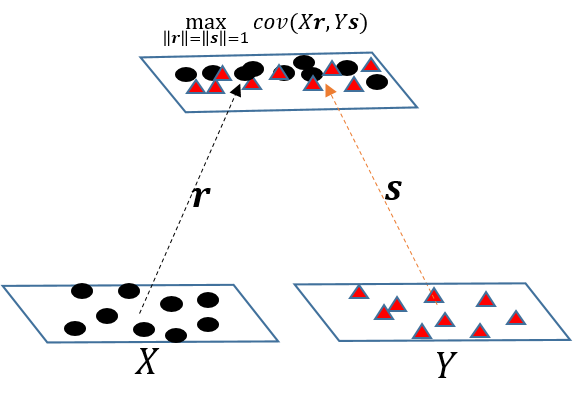
\includegraphics[width=0.5\linewidth]{source/PLS_Euclidean.png}
  	\caption{欧氏空间偏最小二乘回归示意图}
  	\label{fig:PLS_Euclidean}
\end{figure}

最后,这里简单介绍PLS与CCA的关系,更多的关于PLS,PCA,CCA之间的关系可以从\cite{pls_PLSALL}中获得;CCA与PLS作为多元统计分析中的有力工具,广泛应用于统计分析,机器学习,计算机视觉等领域;两者虽然名字差别很大但是形式上却很相近的,以至于在一些情况下可以说两者就是等价的;它们的相似性从它们的数学形式就可以看出来:
\begin{equation}
\label{pls_CCA_VS_PLS}
\begin{split}
&CCA~~:~~\max_{\|\bm{r}\|=\|\bm{s}\|=1}[corr(X\bm{r},Y\bm{s})]^2\\
&PLS~~:~~\max_{\|\bm{r}\|=\|\bm{s}\|=1}[cov(X\bm{r},Y\bm{s})]^2
\end{split}
\end{equation}
上两式的联系,在1976年H. D. Vinod关于canonical ridge analysis的论文\cite{pls_Canonical_ridge}中给出的公式\ref{pls_PCA_CCA_PLS}即可看出一二。
\begin{equation}
\label{pls_PCA_CCA_PLS}
\begin{split}
\max_{\|\bm{r}\|=\|\bm{s}\|=1}\frac{cov(X\bm{r},Y\bm{s})}{([1-\gamma_X]var(X\bm{r})+\gamma_X)([1-\gamma_Y]var(Y\bm{s})+\gamma_Y)}
\end{split}
\end{equation}
其中$0\leq \gamma_X,\gamma_Y \leq 1$,进一步的上述问题的解对应于如下特征值问题:
\begin{equation}
\label{pls_eigenproblem}
([1-\gamma_X]\bm{X^{T}X}+\gamma_X\bm{I})^{-1}\bm{X^{T}Y}([1-\gamma_Y]\bm{Y^{T}Y}+\gamma_Y\bm{I})^{-1}\bm{Y^{T}Xw}=\lambda\bm{w}
\end{equation}
总结上述内容得到:CCA与PLS与在数学形式上很相似,其中PLS最大化的是投影后的向量间的协方差,而CCA最大化的是投影后样本表示的相关系数,两者相差了一个尺度因子,在尺度因子(投影后的标准差)为1的时候两者相等;此外两者本质上都是特征值问题,且特征值问题的一般形式如式\ref{pls_eigenproblem}所示。

\section{黎曼流形上的投影问题}
\label{sec:manifold_projection}
简单回顾欧氏空间中的PCA,CCA和PLS不难发现其中都涉及到投影(如投影向量或投影矩阵)的概念,它是这一类方法的核心,也是本节的主要讨论的对象。这一节的内容主要分为两部分:第一部分从欧氏空间中的投影开始,逐步介绍抽象的投影的概念,然后将这个概念推广到黎曼流形;第二部分会具体的以SPD矩阵流形为例,将黎曼流形的投影的概念具体化。
\subsection{一般化的投影}
\label{sec:common_projection}
这里的投影理解为欧氏空间中高维空间向低维空间的投影的一般化,此外由于PCA,CCA以及PLS中的概念是相似的所以这里就直接以PLS为载体进行欧氏空间中的投影的概念的解释和一般化介绍。

\ref{sec:plsr}节给出了欧氏空间中的偏最小二乘的目标函数的形式是公式\ref{pls_max_cov},也就是最大化协方差的目标。
\begin{equation}
\label{pls_data_MaxCov}
\begin{split}
\max_{\|\bm{r}\|=\|\bm{s}\|=1}[cov(X\bm{r},Y\bm{s})]^{2}&=\max_{\|\bm{r}\|=\|\bm{s}\|=1}\left\{\sum_{i=1}^{n}(\bm{x}_{i}^{T}\bm{r}-\bar{\bm{x}}^{T}\bm{r})(\bm{y}_{i}^{T}\bm{s}-\bar{\bm{y}}^{T}\bm{s})\right\}^2\\
&=\max_{\|\bm{r}\|=\|\bm{s}\|=1}\left\{\sum_{i=1}^{n}[\bm{r}^{T}(\bm{x}_{i}-\bar{\bm{x}})][\bm{s}^{T}(\bm{y}_{i}-\bar{\bm{y}})]\right\}^2\\
\end{split}
\end{equation}
在公式\ref{pls_data_MaxCov}中$\bm{r}^{T}(\bm{x}_{i}-\bar{\bm{x}})$和$\bm{s}^{T}(\bm{y}_{i}-\bar{\bm{y}}),i=1,2,...,n$即为高维空间向低维空间的投影变换。但是这样的概念并不能很好的泛化到流形,因为流形并没有内积的定义。为此,这里先回顾一下欧氏空间中投影的更一般的形式。

高维空间向低位空间的投影的物理意义是在低维空间中找到高维空间中的原始数据最接近的表示。设$\bm{x} \in \mathbb{R}^{n}$是$n$维空间中的向量,又有$S_k$表示$n$维空间中的一个$k$维子空间,那么$\bm{x}$向$S_k$中的投影可以由如\ref{projection}所示的优化问题得到(其中$d(\cdot,\cdot)$表示的是距离函数)。
\begin{equation}
\label{projection}
\begin{split}
\Pi_{S_k}(\bm{x})=\min_{\bm{x}^{\prime} \in S_k}d^{2}(\bm{x}^{\prime},\bm{x})
\end{split}
\end{equation}
特别地,若$S_k$是一维子空间,即$S_k$是由一个向量张成的子空间$S_1=\{\bm{v}|\bm{v}=t\bm{w},t\in \mathbb{R}\text{ and }\bm{w}\in\mathbb{R}^{n}\}$,则投影变换定义如\ref{onedim_projection}所示。
\begin{equation}
\label{onedim_projection}
\begin{split}
&\Pi_{S_1}(\bm{x})=\min_{\bm{x}^{\prime} \in S_1}d^{2}(\bm{x}^{\prime},\bm{x})\\
&t^{*} \triangleq \pi_{S_1}(\bm{x})=\min_{t\in\mathbb{R}}d^{2}(t\bm{w},\bm{x})
\end{split}
\end{equation}
这里的$t$称为投影系数,也就是\ref{pls_data_MaxCov}中的$r^{T}(x_{i}-\bar{\bm{x}})$或$s^{T}(y_{i}-\bar{\bm{y}}),i=1,2,...,N$,因而\ref{pls_data_MaxCov}的问题在这个投影描述下,变成了寻找合适的一维子空间$S_{1}^{x}=\{\bm{v}|\bm{v}=t\bm{r},t\in \mathbb{R}\text{ and }\bm{r}\in\mathbb{R}^{n},\|\bm{r}\|=1\}$,$S_{1}^{y}=\{\bm{v}|\bm{v}=u\bm{s},u\in \mathbb{R}~~{\rm and}~~s\in\mathbb{R}^{n},\|\bm{s}\|=1\}$使得投影后的数据表示具有最大的协方差。
\subsection{对称正定矩阵流形上的均值}
\label{sec:riemannian_mean}
本节将就SPD矩阵流形为例,介绍其上的投影变换;此外总结欧氏空间中的PLS方法,不难发现,若要将PLS推广到黎曼流形需要完成四件事:1)数据的中心化;2)寻找合适的子流形,3)将高维空间中的数据投影到子流形中;4)最大化的协方差。本节的内容主要完成的是前两件事:数据的中心化和寻找合适的子流形。由于子流形的构造与中心化相关,所以本节先花一点篇幅简要回顾SPD上的Karcher mean问题。

由于在本文的第二章中,针对该问题已有详细的的介绍和讨论,所以这里我们直接给出它计算的数学形式。
\begin{displaymath}
\bar{\bm{x}}=\min_x\frac{1}{2n}\sum_{i=1}^{n}\delta^{2}(\bm{x},\bm{x}_i)
\end{displaymath}
这里的$\delta(\cdot,\cdot)$表示的是流形中的测地距离,在PSD流形中常使用也是最基本的就是仿射不便距离(Affine Invariant Distance,AID)\cite{AIM_metric},将AID带入到上式的话得到:
\begin{equation}
\label{AIM_mean}
\begin{split}
\mu&=\min_{X}f(X)=\min_{X}\frac{1}{2n}\sum_{i=1}^{n}\delta^{2}(X,X_i)\\
&=\min_{X}\frac{1}{2n}\sum_{i=1}^{n}\|\log(X^{-\frac{1}{2}}X_iX^{-\frac{1}{2}})\|_F
\end{split}
\end{equation}
其中,由于使用$\mu$来表示样本均值已经是约定俗成的了所以尽管Karcher mean是一个矩阵,这里仍然用$\mu$来表示。第二章已经介绍过要想求出公式\ref{AIM_mean}的解析解几乎是不可能的,但是作为优化问题的话,优化算法仍然是可用的,因此主要的问题就是计算公式\ref{AIM_mean}的梯度函数,在第二章中我们有如下的结果:
\begin{equation}
\label{AIM_grad}
\begin{split}
{\rm dist}(X,X_i)&=\|\log(X^{-\frac{1}{2}} X_i X^{-\frac{1}{2}})\|_{F},i=1,2,...,n\\
\nabla_X {\rm dist}(X,X_i)&=2X^{\frac{1}{2}}\log(X^{\frac{1}{2}}X_{i}^{-1}X^{\frac{1}{2}})X^{\frac{1}{2}}=-2\log_{X}(X_i)
\end{split}
\end{equation}
将上式带入到\ref{AIM_mean}得到:
\begin{equation}
\label{AIM_mean_grad}
\begin{split}
\nabla f(X)&=\frac{1}{2n}\sum_{i=1}^{n}2X^{\frac{1}{2}}\log(X^{\frac{1}{2}}X_{i}^{-1}X^{\frac{1}{2}})X^{\frac{1}{2}}\\
&=-\frac{1}{n}\sum_{i=1}^{n}\log_{X}(X_i)
\end{split}
\end{equation}
利用\ref{AIM_mean_grad}不难得到黎曼流形上的梯度下降更新公式(其中$k$是迭代次数,$\tau$代表步长)。
\begin{equation}
\label{AIM_grad_update}
\mu_{k+1}=\exp_{\mu_k}(\frac{\tau}{n}\sum_{i=1}^{n}\log_{\mu_k}(X_i))
\end{equation}
\subsection{黎曼流形上的子流形与投影}
\label{sec:riemannian_mean}
在\ref{sec:riemannian_mean}节介绍了黎曼流形上的均值的计算,这节将会介绍黎曼流形上高维流形向低维流形的投影的过程,此前在文献\cite{PGA,RCCA}中对该问题就有一些介绍,这里会对之前工作做一个总结,为黎曼流形上的PLS推广做准备。

首先,根据欧氏空间中的高维空间向一维子空间的投影形式(公式\ref{onedim_projection}),可以看出确定一个一维的子流形是投影变换的首要任务,并注意到流形上的测地线是链接两点之间最短的曲线,它是欧氏空间中两点之间直线最短的概念的推广,因此利用测地线构造子流形是自然的一种途径,而从流形上的均值(Karcher mean)出发的测地线常用于构造这样的子流形(目前还没有理论证明这样的构造是最优的,但是一部分在PSD流形上的实验结果验证了在均值这点可以得到不错的结果\cite{RegionCov_pedestrain}),于是将从Karcher mean出发利用测地线构造子空间记为$S_W$,带入到公式\ref{onedim_projection}中并使用测第距离可得到公式\ref{submanifold_projection}的形式。
\begin{equation}
\label{submanifold_projection}
\begin{split}
\Pi_{S_W}(X)=\min_{X^{\prime} \in S_W}\delta^{2}(X^{\prime},X)
\end{split}
\end{equation}
更具体地,当把上述理论运用到对称正定矩阵流形的时候(使用Affine Invariant Distance\cite{AIM_metric}),可以更具体的得到公式\ref{SPD_submanifold}的形式。
\begin{equation}
\label{SPD_submanifold}
\left\{
\begin{split}
\begin{aligned}
&S_W=\exp_\mu({\rm{span}}(W)\cap U)\\
&\Pi_{S_W}(X)=\min_{X^{\prime} \in S_W}\delta^{2}(X^{\prime},X)\\
&~~~~~~~~~~=\min_{t \in (-\epsilon,\epsilon),X^{\prime}=tW}\|\log_{[\exp_{\mu}(tW)]}(X)\|^2\\
&\pi_{S_W}(X)=\min_{t \in (-\epsilon,\epsilon)}\|\log_{[\exp_{\mu}(tw)]}(X)\|^2=t^{*}
\end{aligned}
\end{split}
\right.
\end{equation}
其中$W$就是Karcher mean的切空间中从原点出发的一条切向量,类似于欧氏空间中数据中心化后的空间中的投影方向;公式\ref{SPD_submanifold}即包含了子流形的构造以及原始流形向子流形的投影。为了方便理解这里使用示意图\ref{fig:SPD_SubManifold}
帮助理解。
\begin{figure}
	\centering
	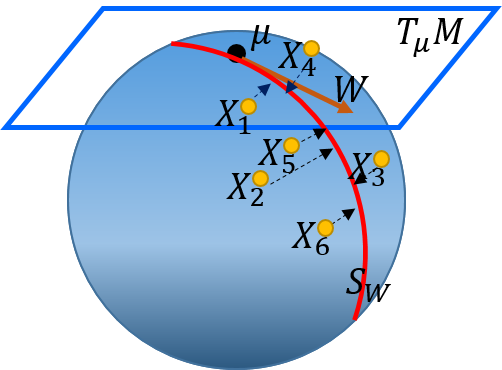
\includegraphics[width=0.5\linewidth]{source/SPD_submanifold.png}
	\caption{流形上的投影示意图}
	\label{fig:SPD_SubManifold}
\end{figure}
\section{黎曼流形上的偏最小二乘回归问题}
\label{sec:RPLS}
本节将借助前面定义的子流形和投影的概念对SPD矩阵流形的一般形式化进行阐述,然后在接下来的一小节中,将结合这种一般化形式针对图像集合分类问题的特点,对其做进一步的改进,使其更加适配到图像集合分类问题上。
\subsection{黎曼流形上偏最小二乘回归问题的一般形式}
\label{sec:RPLS_common}
首先是黎曼流形上的偏最小二乘问题:假设$\{X_i\}_{i=1}^{n},\{Y_i\}_{i=1}^{n} \subset M$是来自对称正定矩阵流形$M$的两组样本,根据公式\ref{submanifold_projection}以及公式\ref{pls_data_MaxCov}这里可以写出如下的目标函数:
\begin{equation}
\label{Riemannian_PLS}
\begin{split}
\max_{w_x,w_y}& C^2(w_x,w_y)=\max_{w_x,w_y}{\left(\sum_{i=1}^{n}(t_i-\bar{t})(u_i-\bar{u})\right)^2}\\
s.t.~~&t_i=\min_{X(t) \in S_{w_x},t \in (-\epsilon,\epsilon)}\delta^{2}(X(t),X_i);i=1,2,..,n;\\
&u_i=\min_{Y(u) \in S_{w_y},u \in (-\eta,\eta)}\delta^{2}(Y(u),Y_i);i=1,2,...,n;\\
&\|w_x\|=\|w_y\|=1;\bar{t}=\frac{1}{n}\sum_{i=1}^{n}t_i;\bar{u}=\frac{1}{n}\sum_{i=1}^{n}u_i.
\end{split}
\end{equation}
将上述的形式化具体到SPD矩阵流形:假设$\{X_i\}_{i=1}^{n},\{Y_i\}_{i=1}^{n} \subset \mathbb{S}_{d}^{+}$是来自对称正定矩阵流形$\mathbb{S}_{d}^{+}$的两组样本,根据公式\ref{SPD_submanifold}以及公式\ref{pls_data_MaxCov}这里可以写出如下的目标函数:
\begin{equation}
\label{SPD_RPLS}
\begin{split}
\max_{W_X,W_Y}& C^2(W_X,W_Y)=\max_{W_X,W_Y}{\left(\sum_{i=1}^{n}(t_i-\bar{t})(u_i-\bar{u})\right)^2}\\
s.t.~~&t_i=\min_{t \in (-\epsilon,\epsilon)}\|\log_{[\exp_{\mu_x}(tW_X)]}(X_i)\|^2;i=1,2,..,n;\\
&u_i=\min_{u \in (-\eta,\eta)}\|\log_{[\exp_{\mu_y}(uW_Y)]}(Y_i)\|^2;i=1,2,...,n;\\
&\|W_X\|=\|W_Y\|=1;\bar{t}=\frac{1}{n}\sum_{i=1}^{n}t_i;\bar{u}=\frac{1}{n}\sum_{i=1}^{n}u_i.
\end{split}
\end{equation}

公式\ref{SPD_RPLS}描述了SPD矩阵流形上的偏最小二乘问题的一般形式,也是定义了流形中的投影之后所能得到的最直接的形式化;但是不难发现还有如下一些问题遗留:1)由于公式\ref{SPD_RPLS}没有解析解,上述问题需要大量的计算,消耗时间过长是一个问题,究其原因主要是$t_i=\min_{t \in (-\epsilon,\epsilon)}\|\log_{[\exp_{\mu_x}(tW_X)]}(X_i)\|^2;i=1,2,..,n;$和$u_i=\min_{u \in (-\eta,\eta)}\|\log_{[\exp_{\mu_y}(uW_Y)]}(Y_i)\|^2;i=1,2,...,n;$的计算过于复杂。2)如何像欧氏空间中的PLS一般计算第二个(或更多个)投影方向(子空间);3)如何将上述问题用于分类问题(或者说如何做回归问题)。在接下来的内容我们将会发现:这些问题中最主要的问题还是原问题没有解析解的问题,当通过适当近似手段将原问题简化后,上面列出的几个问题都将迎刃而解。

前面已经提到优化问题\ref{SPD_RPLS}的计算复杂度过高,并且该问题在图像集合分类问题上会更加严重,原因是数据的维度太高,所以这里选择适当的近似以求在保证一定的精度的同时速度能有较大的提升。

这里的近似的方法在工作\cite{RCCA,PGA}中已有类似的介绍,主要的思想就是针对$t_i=\min_{t \in (-\epsilon,\epsilon)}\|\log_{[\exp_{\mu_x}(tW_X)]}(X_i)\|^2;i=1,2,..,n;$和$u_i=\min_{u \in (-\eta,\eta)}\|\log_{[\exp_{\mu_y}(uW_Y)]}(Y_i)\|^2;i=1,2,...,n;$的计算复杂过高(或者说没有解析解)的问题而提出的简化方案。

以$t_i=\min_{t \in (-\epsilon,\epsilon)}\|\log_{[\exp_{\mu_x}(tW_X)]}(X_i)\|^2$为例,这里我们不难发现时间复杂度主要来自于$\|\log_{[\exp_{\mu_x}(tW_X)]}(X_i)\|^2$而这一部分实际上描述了这样一个过程:将Karcher mean($\mu_x$)的切空间中的向量$tW_X$通过$\exp_{\mu_x}(\cdot)$变换到$\mathbb{S}_{d}^{+}$中然后在$\mathbb{S}_{d}^{+}$中度量$\exp_{\mu_x}(tW_X),X_i$两者的测地距离$\delta(\exp_{\mu_x}(tW_X),X_i)$;据此我们使用如下的近似方案(具体的参考\cite{PGA}),将在原流形中度量$\exp_{\mu_x}(tW_X),X_i$两者的距离改用在$\mu_x$的切空间中度量两者的距离${\rm dist}(\exp_{\mu_x}(tW_X),X_i)\approx \|tW_X-\log_{\mu_x}(X_i)\|_{\mu_x}$,于是原来的投影问题\ref{SPD_submanifold}就变成了:
\begin{equation}
\label{tangent_approxiamte}
\Pi_{S}(X)=\exp\left(\mu_x,\sum_{i=1}^{k}V_i\left<V_i,\log_{\mu_x}(X)\right>\right)\\
\end{equation}
其中$\{V_i\}_{i=1}^{d}$是$\mu_x$处的切空间中的标准正交基($\mu_x$的切空间是内积空间),这点修改使得问题大大简化,稍作整理之后我们可以得到的算法\ref{alg:RPLS_approx}中的对称正定矩阵流形上的偏最小二乘近似算法。
\begin{algorithm}[htb]
\caption{对称正定矩阵流形上的偏最小二乘近似算法}
\label{alg:RPLS_approx}
\begin{algorithmic}[1]
\REQUIRE 对称正定矩阵集合$\bm{X}=\{X_i\}_{i=1}^{n},\bm{Y}=\{Y_i\}_{i=1}^{n}$,需要计算的成分的个数$k$
\ENSURE 在集合$\bm{X}$的Karcher mean($\mu_x$)处的切空间中张成子空间的$k$个成分$\bm{W}_{X}=\{W_{X}^{i}\}_{i=1}^{k}$,以及$\{X_i\}_{i=1}^{n}$对应的投影$\{\bm{t}_i\}_{i=1}^{n}$;在集合$\bm{Y}$的Karcher mean($\mu_y$)处的切空间中张成子空间的$k$个成分$\bm{W}_{Y}=\{W_{Y}^{i}\}_{i=1}^{k}$,以及$\{Y_i\}_{i=1}^{n}$对应的投影$\{\bm{u}_i\}_{i=1}^{n}$;
\STATE 计算$\mu_x, \mu_y$和$\{\hat{X}_i=\log_{\mu_{x}}(X_i)\}_{i=1}^{n}, \{\hat{Y}_i=\log_{\mu_{y}}(Y_i)\}_{i=1}^{n}$
\STATE 利用群操作将样本变换到单位矩阵的切空间:\\
~~~~~~~~~~~~~~~~~~~$\log_{\mu_{x}}(X_i)\rightarrow \mu_{x}^{-1/2}\log_{\mu_{x}}(X_i)\mu_{x}^{-1/2}=\log(\mu_{x}^{-1/2}X_i\mu_{x}^{-1/2})\triangleq \tilde{X}_i$\\
~~~~~~~~~~~~~~~~~~~$\log_{\mu_{y}}(Y_i)\rightarrow \mu_{y}^{-1/2}\log_{\mu_{y}}(Y_i)\mu_{y}^{-1/2}=\log(\mu_{y}^{-1/2}Y_i\mu_{y}^{-1/2})\triangleq \tilde{Y}_i$
\STATE 在$\{\tilde{X}_{i}\}_{i=1}^{n}$以及$\{\tilde{Y}_{i}\}_{i=1}^{n}$之间执行PLS得到$\hat{\bm{W}}_X,\hat{\bm{W}}_Y,T=[\bm{t}_1,\cdots,\bm{t}_k],U=[\bm{u}_1,\cdots,\bm{u}_n]$
\STATE 利用群操作将$\hat{\bm{W}}_X$变换到$\mu_x$的切空间得到$\bm{W}_X$,将$\hat{\bm{W}}_y$变换到$\mu_y$的切空间得到$\bm{W}_Y$
\RETURN $\bm{W}_X,\bm{W}_Y,T,U$
\end{algorithmic}
\end{algorithm}

算法\ref{alg:RPLS_approx}中的:\textit{“在$\{\tilde{X}_{i}\}_{i=1}^{n}$以及$\{\tilde{Y}_{i}\}_{i=1}^{n}$之间执行PLS得到$\hat{\bm{W}}_X,\hat{\bm{W}}_Y,T=[\bm{t}_1,\cdots,\bm{t}_k],U=[\bm{u}_1,\cdots,\bm{u}_n]$”}使用的是欧氏空间中的标准的PLS问题,因为Karcher mean的切空间是内积空间,而通过群操作后的数据在单位阵$I$处的表示也是内积空间,所以欧氏空间中的方法在这里都可以直接使用,进一步的,通过公式\ref{pls_score_model}$\sim$\ref{label_represent}的内容即可得到计算多个成分(投影子空间)和PLS做回归问题的形式化,由于这只是重复前面的内容,这里就不再赘述了,最后在\ref{alg:RPLS_approx_regression}中给出与算法\ref{alg:RPLS_approx}类似的用于回归问题的算法。
\begin{algorithm}[hbt]
\caption{对称正定矩阵流形上的偏最小二乘回归近似算法}
\label{alg:RPLS_approx_regression}
\begin{algorithmic}[1]
\REQUIRE 对称正定矩阵集合$\bm{X}=\{X_i\}_{i=1}^{n}$,label矩阵$Y$,需要计算的成分的个数$k$
\ENSURE 在集合的$\bm{X}$的Karcher mean($\mu$)处的切空间处张成子流形的$k$个成分$\bm{W}_{X}=\{W_{X}^{i}\}_{i=1}^{k}$,以及$\{X_i\}_{i=1}^{n}$对应的投影$\{\bm{t}_i\}_{i=1}^{n}$;欧氏空间中标签集$Y$的投影向量$W_y=\{w_{y}^{i}\}_{i=1}^{k}$及其对应的投影$\{\bm{u}_i\}_{i=1}^{n}$
\STATE 计算$\bm{X}$的Karcher mean($\mu$)以及$\{\hat{X}_i=\log_{\mu}(X_i)\}_{i=1}^{n}$
\STATE 利用群操作将样本移动到单位矩阵的切空间:\\
 ~~~~~~~~~~~~~~~~~~~~$\log_{\mu}(X_i)\rightarrow \mu^{-1/2}\log_{\mu}(X_i)\mu^{-1/2}=\log(\mu^{-1/2}X_i\mu^{-1/2})\triangleq \tilde{X}_i$
\STATE 在$\{\tilde{X}_{i}\}_{i=1}^{n}$以及$Y$之间执行PLS回归得到$\hat{\bm{W}}_x,W_y,T=[\bm{t}_1,\cdots,\bm{t}_k],U=[\bm{u}_1,\cdots,\bm{u}_n]$
\STATE 利用群操作将$\hat{\bm{W}}_x$变换到$\mu$的切空间得到$\bm{W}_x$
\RETURN $\bm{W}_X,W_y,T,U$
\end{algorithmic}
\end{algorithm}
\subsection{面向图像集合分类的黎曼流形上的篇最小二乘回归}
\label{sec:ImageSet_PLS}
这里将算法\ref{alg:RPLS_approx_regression}算法称为基础版本的黎曼流形上的PLS回归,该算法已经可以直接运用到图像集合分类问题了,但是仔细回顾公式\ref{Riemannian_PLS},会发现在计算$t_i,u_i$的时候要求$t_i \in (-\epsilon,\epsilon),u_i \in (-\eta,\eta)$,也就是要求$t_iW_X,u_iW_Y$在$\mu_x,\mu_y$的一个小邻域内,而其本质上是要求SPD矩阵样本的分布是比较集中;这也正是图像集合问题和DTI图像中的Tensor的重要区别之一(图像集合中的样本由于维度高样本少,所以分布往往比较稀疏),也是将黎曼流形上的PLS回归用到图像集合需要解决的问题;此外注意到工作\cite{RCCA,PGA}利用Karcher mean的切空间构造子流形,但是前面已经提到并没有理论证明这样的结果是最好的,所以如果在构造子流形的过程中考虑label的信息相信可以找到更适合构建子流形的地方。接下来的内容是如何针对以上的问题将PLS方法适配到图像集合分类上,并且我们尽量做到在几乎不增加计算复杂度的前提下方法对分类问题的解决有较大的改进。
\subsubsection{融合判别信息的子流形构造}
\label{sec:discrim_single_support}
本节将针对前面提到的第二个问题:找到一个比Karcher mean更具有一定判别性的点构建子流形的我们的解决方案进行说明。具体方案如下,首先注意到公式\ref{AIM_mean}计算Karcher mean的时候是一个无监督的优化过程,所以并未编码判别信息在其中;因此这里考虑编码label到构造子流形的点(相当于算法\ref{alg:RPLS_approx_regression}中的$\mu$),这里为方便起见仍然沿用记号$\mu$。

该步骤的目标是使得在\ref{alg:RPLS_approx_regression}中的$\{X_i\}_{i=1}^{n}$在$\mu$处的切向量表示经过群操作变换到单位阵的切空间中之后的$\{\tilde{X}_i\}_{i=1}^{n}$同类相似度大,异类相似度小,在实际中使用的是cosine相似度,也就是同类的尽量共线,不同类的尽量正交,并保证投影之后“方差”尽量的小(类似于中心化,因为直接进行中心化比较困难,所以在优化的过程要求$\{X_i\}_{i=1}^{n}$在$\mu$处的切向量表示在原切空间($T_{\mu}M$)中应该具有0均值的特点。

沿用之前的记号设$\{X_i\}_{i=1}^{n}$是来自于$C$个类的对称正定矩阵的样本$X_i \in \mathbb{S}_{d}^{+}$,并假设每个类有$n_i,i=1,2,\cdots,C$个样本$n=\sum_{i=1}^{C}n_i$,样本的label我们用公式\ref{label_represent}的矩阵$Y$表示,下面是编码判别信息的形式化过程。
\begin{itemize}
\item 定义平方相似度矩阵$F=[\rho_{ij}^{2}]_{n\times n},\rho_{ij}=\frac{k_{ij}}{\sqrt{k_{ii}k_{jj}}}$,其中$k_{ij}$由下式定义:
\begin{equation}
\begin{split}
k_{ij}&=\left<\tilde{X}_i,\tilde{X}_j\right>\\
&=\left<\log(\mu^{-1/2}X_i\mu^{-1/2}),\log(\mu^{-1/2}X_j\mu^{-1/2})\right>\\
&=\left<\log(\mu^{1/2}X_{i}^{-1}\mu^{1/2}),\log(\mu^{1/2}X_{j}^{-1}\mu^{1/2})\right>\\
\end{split}
\end{equation}
\item 定义矩阵$P^{\prime}=1-2YY^{T}$,进一步的为了平衡正负样本对之间($P^{\prime}$中的1的个数和-1的个数)的比例,这里做一下平衡操作:设$n_{\#1}$=\{$P^{\prime}$中1的个数\},$n_{\#-1}$=\{$P^{\prime}$中-1的个数\}则定义平衡后的矩阵为$P$,其中:
\begin{equation}
P_{ij}=\left\{
\begin{split}
&\frac{P_{ij}^{\prime}}{n_{\#1}},if~~P_{ij}^{\prime}=1\\
&\frac{P_{ij}^{\prime}}{n_{\#-1}},if~~P_{ij}^{\prime}=-1
\end{split}
\right.
\end{equation}
\item 根据工作\cite{PGA},这里定义“方差”:$\frac{1}{n}\sum_{i=1}^{n} \|\log_{\mu}(X_i)\|^2$
\item 最后的目标函数为:
\begin{equation}
\label{support_search}
\min_{\mu}f(\mu)={\rm tr}(FP^{T})+\frac{\lambda}{n}\sum_{i=1}^{n} \|\log_{\mu}(X_i)\|^2,\mu \succ 0
\end{equation}
其中$\lambda$是一个平衡因子起到平衡两者权重的作用,同时也有平衡量纲的作用,避免其中一方因量纲问题绝对占优。
\end{itemize}
\subsubsection{融合判别信息的切空间构造问题的优化}
\label{sec:discrim_single_support_opt}
公式\ref{support_search}没有解析解因此需要通过需要通过优化来求解,而且约束条件$\mu \succ 0$表明了问题的解空间是$\mathbb{S}_{d}^{+}$,这里我们使用黎曼流形上的共轭梯度算法(conjugate gradient methods\ref{alg:Manifold_Gradient_Descend})来优化问题\ref{support_search},关于黎曼流形上的共轭梯度算法可以参看本文的第二章以及文献\cite{Conjugate_Gradient_Survery},使用该方法优化的时候,最主要的输入就是\ref{support_search}的导数。接下来将利用第二章的内容对公式\ref{support_search}的导数计算作简要说明。

公式\ref{support_search}主要包含两部分:${\rm tr}(FP^{T})$和$\frac{\lambda}{n}\sum_{i=1}^{n} \|\log_{\mu}(X_i)\|^2$;这里先对第一部分的导数进行计算:
\begin{equation}
\label{support_search_part1_gradeint}
\begin{split}
{\rm tr}(FP^{T})&=\sum_{i=1}^{n}\sum_{j=1}^{n}F_{ij}P_{ij}=\sum_{i=1}^{n}\sum_{j=1}^{n}P_{ij}\frac{k_{ij}^2}{k_{ii}k_{jj}}\\
\frac{\partial}{\partial \mu}{\rm tr}(FP^{T})&=\sum_{i=1}^{n}\sum_{j=1}^{n}P_{ij}\left(c_1\frac{\partial}{\partial \mu}k_{ij}-c_2\frac{\partial}{\partial \mu}k_{ii}-c_3\frac{\partial}{\partial \mu}k_{jj}\right)\\
{\rm where~~}c_1&=\frac{2k_{ij}k_{ii}k_{jj}}{(k_{ii}k_{jj})^2},c_2=\frac{k_{ij}k_{ij}k_{jj}}{(k_{ii}k_{jj})^2},c_3=\frac{k_{ij}k_{ij}k_{ii}}{(k_{ii}k_{jj})^2}
\end{split}
\end{equation}
公式\ref{support_search_part1_gradeint}表明导数的计算的核心主要是$\frac{\partial}{\partial \mu}k_{ij}$,因此剩下的工作主要就是$k_{ij}$的导数计算;在此之前这里先对$k_{ij}$的形式稍加变换,这样会比较方便理解后面的$k_{ij}$的导数的形式(公式\ref{kernel_elementwise_gradient}):
\begin{equation}
\label{kernel_elementwise}
\begin{split}
&\left<\log_{\mu}(X_i),\log_{\mu}(X_j)\right>_{\mu}\\
&~~~~~~=\left<\log(\mu^{-1/2}X_{i}\mu^{-1/2}),\log(\mu^{-1/2}X_j\mu^{-1/2})\right>\\
&~~~~~~=\left<\log(\mu^{1/2}X_{i}^{-1}\mu^{1/2}),\log(\mu^{1/2}X_{j}^{-1}\mu^{1/2})\right>\\
&~~~~~~={\rm tr}(\log(X_{i}^{-1}\mu)\log(X_{j}^{-1}\mu))\\
&~~~~~~={\rm tr}(X_{i}^{-1/2}\log(X_{i}^{-1/2}\mu X_{i}^{-1/2})X_{i}^{1/2}X_{j}^{-1/2}\log(X_{j}^{-1/2}\mu X_{j}^{-1/2})X_{j}^{1/2})\\
&~~~~~~={\rm tr}(\log(X_{i}^{-1/2}\mu X_{i}^{-1/2})X_{i}^{1/2}X_{j}^{-1/2}\log(X_{j}^{-1/2}\mu X_{j}^{-1/2})X_{j}^{1/2}X_{i}^{-1/2})\\
&~~~~~~=\left<\log(X_{i}^{-1/2}\mu X_{i}^{-1/2}),X_{i}^{1/2}X_{j}^{-1/2}\log(X_{j}^{-1/2}\mu X_{j}^{-1/2})X_{j}^{1/2}X_{i}^{-1/2}\right>\\
\end{split}
\end{equation}
下面给出$k_{ij}$的导数的具体形式,由于比较复杂,感兴趣的读者可以参看本文第二章以及文献\cite{Maniopt_DiscreteCurveFitting,Statistics_SLEDML}的相关章节。
\begin{equation}
\label{kernel_elementwise_gradient}
\begin{split}
&\frac{\partial}{\partial \mu}k_{ij}=X_{i}^{-1/2}\left(D\log(X_{i}^{-1/2}\mu X_{i}^{-1/2})[sym(X_{i}^{1/2}X_{j}^{-1/2}\log(X_{j}^{-1/2}\mu X_{j}^{-1/2})X_{j}^{1/2}X_{i}^{-1/2}]\right)X_{i}^{-1/2}\\
&~~~~~~+X_{j}^{-1/2}\left(D\log(X_{j}^{-1/2}\mu X_{j}^{-1/2})[sym(X_{j}^{1/2}X_{i}^{-1/2}\log(X_{i}^{-1/2}\mu X_{i}^{-1/2})X_{i}^{1/2}X_{j}^{-1/2}]\right)X_{j}^{-1/2}\\
\end{split}
\end{equation}

至于第二部分的$\frac{\lambda}{n}\sum_{i=1}^{n} \|\log_{\mu}(X_i)\|^2$的导数,不难发现以下的关系$\|\log_{\mu}(X_i)\|^2=\left<\log_{\mu}(X_i),\log_{\mu}(X_i)\right>_{\mu}=k_{ii}$,因此这部分的导数可以根据\ref{kernel_elementwise_gradient}直接导出来。
\begin{equation}
\label{support_search_part2_gradeint}
\begin{split}
\frac{\partial}{\partial \mu}\frac{\lambda}{n}\sum_{i=1}^{n} \|\log_{\mu}(X_i)\|^2=\frac{\lambda}{n}\sum_{i=1}^{n}\frac{\partial}{\partial \mu}k_{ii}
\end{split}
\end{equation}
整合两部分的结果可以得到公式\ref{support_search}在普通欧氏空间中关于$\mu$的导数如公式\ref{support_search_gradeint}所示。
\begin{equation}
\label{support_search_gradeint}
\nabla_{\mu} f(\mu)=\sum_{i=1}^{n}\sum_{j=1}^{n}P_{ij}\left(c_1\frac{\partial}{\partial \mu}k_{ij}-c_2\frac{\partial}{\partial \mu}k_{ii}-c_3\frac{\partial}{\partial \mu}k_{jj}\right)+\frac{\lambda}{n}\sum_{i=1}^{n}\frac{\partial}{\partial \mu}k_{ii}
\end{equation}
最后,利用第二章中的内容以及论文\cite{Statistics_SLEDML,Maniopt_DiscreteCurveFitting}中的结果将普通的梯度转换为黎曼梯度。这只需要对公式\ref{support_search_gradeint}作公式\ref{support_search_riemannian_gradeint}中的变化即可:
\begin{equation}
\label{support_search_riemannian_gradeint}
{\rm grad}_{\mu}f(\mu)=\mu \nabla_{\mu} f(\mu) \mu
\end{equation}
将优化公式\ref{support_search}得到的$\mu$代替算法\ref{alg:RPLS_approx_regression}中的Karcher mean并在该点做投影变化,即得到了融入判别信息的改进方法;虽然目前的结果不是本文所提算法的最终形式,但是这是最终算法的基础,在后面的章节中将会反复使用到,所以这里将其总结在算法\ref{alg:RPLS_discrim_tangent_approx_regression}中。
\begin{algorithm}
\caption{对称正定矩阵流形上具有判别性的切空间偏最小二乘回归近似算法}
\label{alg:RPLS_discrim_tangent_approx_regression}
\begin{algorithmic}[1]
\REQUIRE 对称正定矩阵集合$\bm{X}=\{X_i\}_{i=1}^{n}$,label矩阵${Y}$,需要计算的成分的个数$k$
\ENSURE 融入判别性的切空间$T_{\mu}M$对应的$\mu$,集合$\bm{X}$在$T_{\mu}M$中的$k$个成分$\bm{W}_X=\{W_{X}^{i}\}_{i=1}^{k}$,以及$\{X_i\}_{i=1}^{n}$对应的投影$\{\bm{t}_i\}_{i=1}^{n}$;欧氏空间中标签集$\bm{Y}$的投影向量$W_y=\{\bm{w}_{y}^{i}\}_{i=1}^{k}$及其对应的投影$\{\bm{u}_i\}_{i=1}^{n}$
\STATE 初始化$\mu=\mu_0$(通常为$I$)求解最小化问题2.1获得$\mu$,然后计算$\{\hat{X}_i=\log_{\mu}(X_i)\}_{i=1}^{n}$
\STATE 利用群操作将样本移动到单位矩阵的切空间:\\
 ~~~~~~~~~~~~~~~~~~~~$\log_{\mu}(X_i)\rightarrow \mu^{-1/2}\log_{\mu}(X_i)\mu^{-1/2}=\log(\mu^{-1/2}X_i\mu^{-1/2})\triangleq \tilde{X}_i$
\STATE 在$\{\tilde{X}_{i}\}_{i=1}^{n}$以及${Y}$之间执行PLS回归得到$\hat{\bm{W}}_X,W_y,T=[\bm{t}_1,\cdots,\bm{t}_k],U=[\bm{u}_1,\cdots,\bm{u}_n]$
\STATE 利用群操作将$\hat{W}_x$变换到$\mu$的切空间得到$\bm{W}_x$
\RETURN $\bm{W}_X,W_y,T,U$
\end{algorithmic}
\end{algorithm}
最后,为了方便理解\ref{alg:RPLS_discrim_tangent_approx_regression}算法这里使用利用示意图\ref{fig:discrim_tangent_RPLS}对算法的思想进行说明。
\begin{figure}
	\centering
	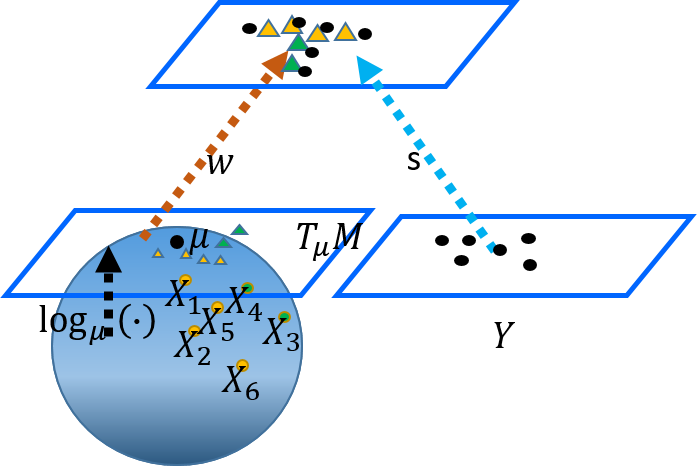
\includegraphics[width=0.5\linewidth]{source/Discrim_Tangent_PLS.png}
	\caption{算法\ref{alg:RPLS_discrim_tangent_approx_regression}的示意图}
	\label{fig:discrim_tangent_RPLS}
\end{figure}
\subsubsection{多切空间逐步回归的偏最小二乘方法}
\label{sec:muliti_tangent_rpls}
注意到算法\ref{alg:RPLS_discrim_tangent_approx_regression}仍然没有解决一开始提到的另一个问题:数据不紧凑所带来的近似/估计不准问题,接下来的部分将针对这个问题做进一步的改进。公式\ref{SPD_RPLS}中的$t_i \in (-\epsilon,\epsilon)$和$u_i \in (-\eta,\eta)$的条件就是要求样本数据需要足够集中才行,但是如果直接将算法\ref{alg:RPLS_discrim_tangent_approx_regression}中的$\bm{t}_i$或$\bm{u}_i$进行截断的话,这不仅会损失精度(因为原始数据本来分布很稀疏,再限制$t_i$或$u_i$的取值范围无疑会使得估计更加的不准),而且在优化的时候也会比较麻烦,所以这里考虑寻找多个点使用多个切空间来缓解数据稀疏的问题。在这样的框架下,每个切空间并不需要很强的表示能力,只需要能够反应原始数据的一部分结构就行,而最后通过设计特定的方法整合每个切空间中的表示模型得到更具表示能力的模型帮助判别(分类)问题的研究。

上述框架的主要问题是如何选取各个切空间以及如何将他们有效的融合起来,这里我们使用逐步回归的方案来同时解决这两个问题:对算法\ref{alg:RPLS_discrim_tangent_approx_regression}中的数据$\bm{X}=\{X_i\}_{i=1}^{n}$和label矩阵${Y}$执行算法\ref{alg:RPLS_discrim_tangent_approx_regression}得到获得一个切空间$T_{\mu_1}M$及其对应的$k$个投影方向$\bm{W}_{X}^{(1)},W_{y}^{(1)}$和对应的$T_{1},U_{1}$;然后对$\{\tilde{X}_{i=1}^{n}\}$以及$Y$利用公式\ref{pls_deflate}进行defalte操作:%$\underrightarrow{abc}$,
$\{\tilde{X}_{i}\}_{i=1}^{n} \xlongrightarrow{defalte} \{\tilde{X}^{res}_i\}_{i=1}^{n},{Y}\xlongrightarrow{defalte} {Y}^{res}$,然后对$\{\tilde{X}^{res}_{i}\}_{i=1}^{n}$利用群操作从单位阵处将数据变换到$\mu$再用$\exp_{\mu_{1}}(\cdot)$将数据$\{\tilde{X}^{res}_i\}_{i=1}^{n}$变换到SPD矩阵流形得到$\{Z^{res}_{i}\}_{i=1}^{n}$,最后将$\{Z^{res}_i\}_{i=1}^{n},{Y}^{res}$赋值给$\bm{X}=\{X_i\}_{i=1}^{n}$和$Y$,并重新初始化$\mu_2$后开始第二次迭代;反复上述过程直到获得指定个数的切空间,算法终止。将上述过程用算法\ref{alg:RPLS_multi_support_approx_regression}描述。
\begin{algorithm}[htb]
\caption{对称正定矩阵流形上多切空间偏最小二乘回归近似算法}
\label{alg:RPLS_multi_support_approx_regression}
\begin{algorithmic}[1]
\REQUIRE 对称正定矩阵集合$\bm{X}=\{X_i\}_{i=1}^{n}$,label矩阵${Y}$,每个切空间计算的成分的个数$k$,指定切空间的个数$p$
\ENSURE 融入判别性的$p$个切空间$T_{\mu_1}M,\cdots,T_{\mu_{p}}M$对应的$\mu_{1},\cdots \mu_{p}$,数据$\bm{X}$在$T_{\mu_1}M,\cdots,T_{\mu_{p}}M$中各自的$k$个成分$\bm{W}_{x}^{(1)},\cdots,\bm{W}_{x}^{(p)}$,以及对应的投影$T_1,\cdots,T_{p}$;欧氏空间中标签集${Y}$逐次回归的投影矩阵$W_{y}^{(1)},\cdots,W_{y}^{(p)}$及其对应的投影$U_1,\cdots,U_{p}$
\STATE 初始化$output$为包含$p$个cell的结构:$output=cell(1,p)$
\FOR{$j=1;~j\leq p;~j=j+1$}
	\STATE 初始化$\mu_j=\mu_0$(通常为$I$)最小化2.1问题获得$\mu_j$,然后计算$\{\hat{X}_i=\log_{\mu_j}(X_i)\}_{i=1}^{n}$
	\STATE 利用群操作将样本移动到单位矩阵的切空间:\\
 	~~~~~~~~~~~~~~~~~~~~$\log_{\mu_{j}}(X_i)\rightarrow \mu_{j}^{-1/2}\log_{\mu}(X_i)\mu_{j}^{-1/2}=\log(\mu_{j}^{-1/2}X_i\mu_{j}^{-1/2})\triangleq \tilde{X}_i$
	\STATE 在$\{\tilde{X}_{i}\}_{i=1}^{n}$以及$\bm{Y}$之间执行PLS回归得到:\\
	$\hat{\bm{W}}_{x}^{(j)},W_{y}^{(j)},T_{j}=[\bm{t}_{1}^{j},\cdots,\bm{t}_{k}^{j}],U_j=[\bm{u}_{1}^{j},\cdots,\bm{u}_{k}^{j}]$
	\STATE 利用群操作将$\hat{\bm{W}}_{x}^{(j)}$变换到$\mu_{j}$的切空间得到$\bm{W}_{x}^{(j)}$
	\STATE 对$\bm{X},{Y}$使用deflate操作:$\{\tilde{X}_{i}\}_{i=1}^{n} \xlongrightarrow{defalte} \{\tilde{X}^{res}_{i}\}_{i=1}^{n},{Y}\xlongrightarrow{defalte} {Y}^{res}$
	\STATE 利用群操作从单位阵处将数据$\{\tilde{X}^{res}_{i}\}_{i=1}^{n}$变换到$\mu_{j}$然后用$\exp_{\mu_{j}}(\cdot)$将结果变换到SPD矩阵流形得到$\{Z^{res}_{i}\}_{i=1}^{n}$
	\STATE 将$\{Z^{res}_{i}\}_{i=1}^{n},{Y^{res}}$赋值给$\bm{X}=\{X_i\}_{i=1}^{n}$和${Y}$
	\STATE 保存此次结果:$[\mu_{j},\bm{W}_{x}^{(j)},W_{y}^{(j)},T_{j},U_{j}]\rightarrow output\{j\}$
\ENDFOR
\RETURN $output$
\end{algorithmic}
\end{algorithm}

为了帮助理解,与前面类似,这里同样用一个示意图对算法\ref{alg:RPLS_multi_support_approx_regression}的核心进行描述说明,具体如图\ref{fig:multi_discrim_tangent_PLS}所示。
\begin{figure}[bht]
	\centering
	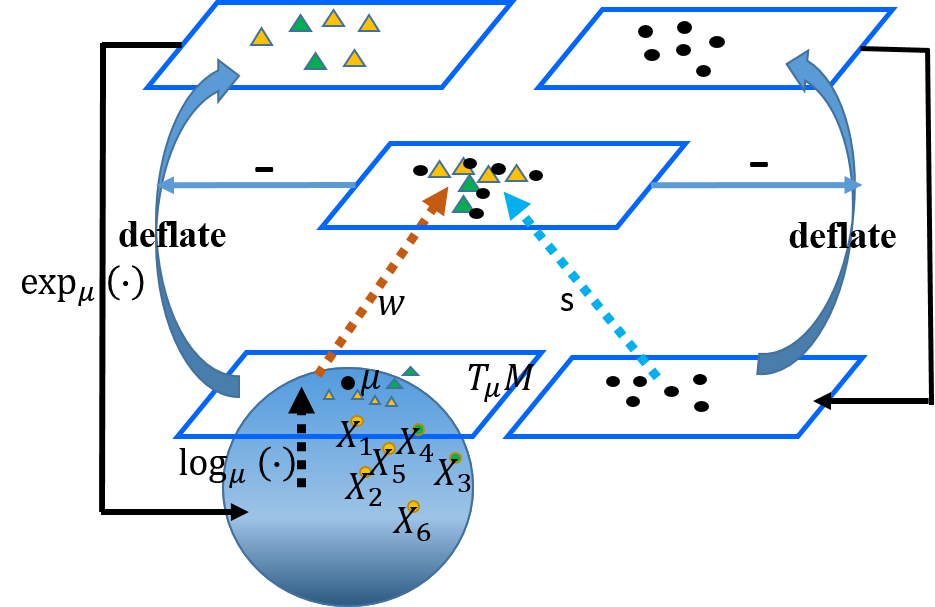
\includegraphics[width=0.7\linewidth]{source/multi_discrim_tangent_PLS.png}
	\caption{算法\ref{alg:RPLS_multi_support_approx_regression}的示意图}
	\label{fig:multi_discrim_tangent_PLS}
\end{figure}

在训练数据上运用算法\ref{alg:RPLS_multi_support_approx_regression}的到训练参数后,测试的部分与普通的算法\ref{alg:RPLS_discrim_tangent_approx_regression}或\ref{alg:RPLS_approx_regression}的测试类似,所不同的是算法\ref{alg:RPLS_multi_support_approx_regression}中回归的$Y$是所有切空间中结果的综合(逐步回归相加)得到的。

关于训练,算法\ref{alg:RPLS_multi_support_approx_regression}与\ref{alg:RPLS_discrim_tangent_approx_regression}和\ref{alg:RPLS_approx_regression}有些许的不同:首先是算法\ref{alg:RPLS_multi_support_approx_regression}的参数$k$的选择往往要比后两者的小很多,例如在YTC\cite{Database_YTC}数据集上算法\ref{alg:RPLS_approx_regression}和\ref{alg:RPLS_discrim_tangent_approx_regression}的参数$k$默认设置为类别数减一(46=47-1)且实验发现减小$k$会使得算法的性能降低,而算法\ref{alg:RPLS_multi_support_approx_regression}中$k$的选择为26,过高或过低都会降低算法的性能(原因可能是欠拟合或过拟合了);算法\ref{alg:RPLS_multi_support_approx_regression}的另一个重要的参数的选择就是$p$,这个也会有欠拟合和过拟合的现象;最后是在测试的时候发现,数据是否中心化对算的最终结果也有一定的影响,这个问题在UIUC\cite{Database_UIUC}数据上做材料分类的时候尤其明显。
\section{实验验证}
\label{sec:RPLS_exp}
前面的章节对问题的背景,已有的方法,存在的问题以及本文的动机和针对问题的解决的方案等做了阐述,本节将会实验验证前面的方法并从实验结果出发分析方法的特点和存在的问题等。

本实验主要从以下几个计算机视觉的任务进行验证:物体识别(数据库ETH80\cite{Database_ETH80}),材料分类(数据库UIUC\cite{Database_UIUC})以及视频人脸识别(数据集YTC\cite{Database_YTC});由于这些数据集已经在\ref{sec:data_intro}节进行了介绍,并且这些数据集的测试协议也已经在\ref{sec:data_intro}节中介绍,所以这里就不再进行阐述,如果读者对数据或测试协议有什么不明的话可以到\ref{sec:data_intro}一节进行查看。
\subsection{原始特征构造}
\label{Database_feature}
这里将简单的介绍一下,各个任务对应的数据集上的基本特征的构造,这些特征底层特征的提取将用于最后的SPD矩阵(实际上也可看作是一种特征表示)的构造。首先,在用于物体识别的ETH80\cite{Database_ETH80}数据集上,所有的图片被预先被resize成$20\times 20$的大小图片,然后灰度特征被直接用于物体识别任务;在材料识别任务的UIUC\cite{Database_UIUC}数据集上,这里使用Region Covariance\cite{RegionCov}表示一张图片,参考\cite{Statistics_SPDML},这里的Region Covariance 的构造中我们使用128维的dense SIFT\cite{SIFT}特征作为基本的特征:首先将图片resize到$400\times400$然后,以4个像素为间隔(每个块的大小为$16 \times 16$,共8个角度,4个bin)划分网格,在每个网格点128维的SIFT特征被提取作为构造Region Covariance的基本特征(与工作\cite{Statistics_SPDML}中的不同的是工作\cite{Statistics_SPDML}还融合了颜色特征);最后在视频人脸识别任务的数据库YTC\cite{Database_YTC}上,首先将图片resize到$20\times 20$然后直方图均衡化被用于鲁棒的特征构造。
\subsection{对称正定矩阵表示的构造}
\label{sec:Database_SPD_Construct}
在“原始特征构造\ref{Database_feature}”这一小节介绍了基本的图像特征的提取和预处理方式,在本节中将对使用这些基本特征构造SPD矩阵表示做简要的介绍:首先是材料识别任务的UIUC\cite{Database_UIUC}数据集上的SPD表示,由于使用的是Region Covariance\cite{RegionCov},这里使用的是标准的构造方式,故不再做进一步介绍,有兴趣的读者可以参看文献\cite{RegionCov};在物体识别的ETH80\cite{Database_ETH80}和视频人脸识别的\cite{Database_YTC}数据集上,这里根据工作\cite{Statistics_CDL}中的内容使用SPD矩阵表示图像集合,但是稍微有些不同的是:根据\cite{Statistics_HERML,Statistics_DARG}中的构造方式,均值的信息也被融入了图像集合的SPD特征表示当中(公式\ref{MeanCov_SPD_Construct}中的$\Sigma$是样本协方差,$\bm{m}$是样本均值,$d$是样本的维数):
\begin{equation}
\label{MeanCov_SPD_Construct}
C={\rm det}(\Sigma)^{-\frac{1}{d+1}}\left[
\begin{array}{cc}
\Sigma+\bm{m}\bm{m}^{T}&m\\
\bm{m}&1
\end{array}
\right]
\end{equation}
最后还需要一提的是对于所有的原始特征实验中都做了$95\%$的PCA降维处理;对于样本协方差矩阵$\Sigma$奇异的时候(往往是由于样本个数小于样本维度造成的),根据\cite{Statistics_DARG,Statistics_LEML}中的做法,一个小的正的正则项:$\delta\bm{I},\delta=10^{-3}\times {\rm tr}(C)$(其中$\bm{I}$是单位阵)被加到$\Sigma$上:$\Sigma+\delta\bm{I}\rightarrow \Sigma$。
\subsection{实验结果与分析}
\label{sec:RPLS_exp_result_analysis}
在本实验中,我们将本文所提的方法统一用缩写RPLS(Riemannian Partial Least Squear regression,黎曼偏最小二乘方法)表示,本小结的内容是RPLS方法在物体识别,材料识别以及视频人脸识别三个任务上的实验结果呈现,在对比方法中我们选取了具有代表性的方法:基于PLS的协方差判别学习方法(Covariance Discriminant Learning,CDL)\cite{Statistics_CDL},黎曼稀疏编码学习的方法(Riemannian Sparse Representation,RSR),然后是发表在2014年欧洲计算机视觉会议(European Conference On Computer Vision,ECCV)上的工作:对称正定矩阵流形学习(SPD-Manifold Learning,SPDML)在两种度量(Stein Divergence\cite{Stein_divergence}和Affine Invariant Metric\cite{AIM_metric})下的方法,以及使用分布函数建模集合的方法DARG\cite{Statistics_DARG}和BeyondGauss\cite{Statistics_BeyondGauss}以及SPD矩阵流形上的度量学习(Metric Learning)方法LEML\cite{Statistics_LEML}。表\ref{tab:RPLS_experiment}给出了这些方法在三个任务上的实验对比结果,其中所有的结果均是按照\ref{sec:data_intro}节的协议获得的,对于其它文章的方法,这里从作者的主页上获得源代码并小心的调整参数后报告的是在\ref{sec:data_intro}节的协议下所获得的最好的结果。
\begin{table}[htb]
	\centering
	\caption{黎曼流形上的PLS回归算法实验结果}
	\begin{tabular*}{\linewidth}{@{\extracolsep{\fill}}|l|ccc|}\hline
		\diagbox{方法}{数据集} &ETH80 &UIUC &YTC \\ \hline
		CDL-PLS\cite{Statistics_CDL} &93.25$\pm$4.72 &53.89$\pm$4.06 &70.28$\pm$2.13 \\ \hline
		RSR-Stein\cite{Dictionary_RSR} &93.25$\pm$3.34 &52.41$\pm$4.03 &72.77$\pm$2.69  \\ \hline
		SPDML-Stein\cite{Statistics_SPDML} &90.50$\pm$3.87 &49.17$\pm$2.37 &61.57$\pm$3.43  \\ \hline
		SPDML-AIM\cite{Statistics_SPDML} &90.75$\pm$3.34 &48.09$\pm$1.82 &64.66$\pm$2.92  \\ \hline
		BeyondGauss\cite{Statistics_BeyondGauss} &84.75$\pm$6.29 &N/A &71.46$\pm$2.61  \\ \hline
		DARG\cite{Statistics_DARG} &92.25$\pm$2.19 &N/A &77.09$\pm$1.92  \\ \hline
		LEML\cite{Statistics_LEML}&94.75$\pm$2.49 &48.98$\pm$3.69 &70.53$\pm$2.95  \\ \hline
		$\rm \bm{RPLS_{single}}$ &\textbf{92.75$\pm$4.32} &\textbf{54.72$\pm$3.61} &\textbf{74.48$\pm$2.79}  \\ \hline
		$\rm \bm{RPLS_{multi}}$ &\textbf{95.50$\pm$2.58} &\textbf{56.57$\pm$3.49} &\textbf{77.33$\pm$2.95}  \\ \hline
	\end{tabular*}
	\label{tab:RPLS_experiment}
\end{table}

其中,$\rm RPLS$算法的下标表示的基础版本的黎曼流形上的PLS算法\ref{alg:RPLS_discrim_tangent_approx_regression}($\rm \bm{RPLS_{single}}$)还是多切空间逐步回归的算法\ref{alg:RPLS_multi_support_approx_regression}($\rm \bm{RPLS_{multi}}$)。最终的实验结果验证了我们最初的猜想,多切空间偏最小二乘回归算法在三个任务上都获得了state-of-the-art的结果;我们将取得这样的结果的原因归结为(与CDL\cite{Statistics_CDL}相比):1)首先是按照公式\ref{MeanCov_SPD_Construct}构造的SPD表示中均值信息者带来了一定性能上的提升;2)考虑切空间的选择带来了表格倒数第二行和表格第一行的变化(因为CDL-PLS与在单位阵切空间中的$\rm \bm{RPLS_{single}}$是等价的);3)最后是单切空间与多切空间的方案差别带来了表格中最后两行的变化,同时也力证多切空间逐步回归算法\ref{alg:RPLS_multi_support_approx_regression}的有效性。

试验中我们发现公式\ref{support_search}中的第二项对算法性能有小幅的提升,试验中我们始终固定公式中$\lambda=0.001$。而在前面我们也有介绍,算法\ref{alg:RPLS_multi_support_approx_regression}中的参数$k,p$对于算法的影响较大,也是本算法需要改进的一大方向。

最后在对比的一系列的方法中,BeyondGauss\cite{Statistics_BeyondGauss}的方法由于是使用KDE来估计分布函数,而在UIUC\cite{Database_UIUC}这个数据集上原始的特征是Dense Sift(样本非常多),直接导致了无法计算的问题,所以这里的结果没有汇报(N/A),其它的结果是在hellinger散度下的结果。同样由于内存问题GARG方法在UIUC数据集上也无法获得结果,所以也使用N/A代替。表格中对比方法的结果都是从作者主页获取的代码小心调参后获得的最好的结果。
\section{总结与下一步工作}
\label{sec:conclusion_futurework}
本章从子流形与投影的概念出发,参考相关工作\cite{PGA,RCCA,AIM_metric,Statistics_CDL}等首先导出了黎曼流形上的偏最小二乘问题以及偏最小二乘用于回归的一般形式,然后以SPD矩阵流形为例将算法形式化到\ref{alg:RPLS_approx_regression}中,并针对图像集合分类问题与DTI(Diffusion Tensor Images)的不同(主要是数据更稀疏的问题),提出了两点通用的改进(这里之所以说是通用的改进,是因为即便数据聚集在流形的小范围内这些改进依然是适用的)得到了多切空间偏最小二乘回归算法,使得算法可以适应这种数据稀疏的情况,最后的实验验证部分验证了方法的有效性。

实验分析部分以及算法\ref{alg:RPLS_multi_support_approx_regression}分析部分都提到,算法\ref{alg:RPLS_multi_support_approx_regression}中的参数$k,p$太大会过拟合太小又会欠拟合,分析其原因的话可能是逐步回归的方式没能有效的组合各个切空间中的信息,接下来可能参考\cite{RegionCov_pedestrain}中的方法使用Adaboost的框架进行多个切空间中模型的组合。
% create on 2016-03-14,the third chapter of thesis: Fixed-rank PSD流形判别学习方法
\chapter{低秩对称半正定矩阵判别学习方法}
\label{chap:PSD_discrim_learning}
前面的章节已经提到,统计建模图像集合的方法中有相当一部分的模型都是与样本协方差矩阵有关,但样本协方差矩阵的计算中一个很现实的问题是样本数往往小于数据维度,因为即使是$20\times 20$的小图像也有400维,也就是说至少需要400个样本才有可能使得样本协方差矩阵是非奇异的;这不管是对多视角图像的图片集合还是对视频监控(400帧的图像在30FPS的帧率下也需要13秒还多)中的视频都是很苛刻的要求。因此实际中获得的样本协方差矩阵实际上是对称半正定(Positive Semi-Definite, PSD)矩阵。在使用样本协方差矩阵建模图像集合的方法中,针对该问题的一个常用的trick是给样本协方差矩阵的对角线上加上一个正则项(如\ref{sec:Database_SPD_Construct}中介绍的一样);但是这并没从本质上解决样本协方差矩阵奇异的问题,这促使本文回到数据所在的原始集合——对称半正定矩阵集合中研究图像集合的建模和判别学习问题。

%注意到,虽然原始的对称半正定(PSD)矩阵空间是一个凸集合,但是以目前了解到的情况而言,无约束的对称半正定集合上并没有很好的定义的数学结构,与之最接近的一个数学结构是Fixed-Rank PSD集合(公式\ref{Fixed-Rank-PSD-set}),这也是我们早期的主要研究对象。
%\begin{equation}
%\label{Fixed-Rank-PSD-set}
%\mathbb{S}_{d}^{+}(k)=\{A|A\in \mathbb{R}^{n \times n},A=A^{T},\langle Ax,x\rangle \geq 0,\forall x \in \mathbb{R}^n;{\rm rank}(A)=k\}
%\end{equation}
%如果在该结构上定义合适的黎曼度量的话就可以使得该集合形成一个黎曼流形结构\cite{PSD_Riemannian};
另一方面,当使用对称正定矩阵表示图像集合的时候,对称正定矩阵的维度往往非常高,如$20 \times 20$的图像组成的集合,它的样本协方差将达到$400\times 400$的规模,这对存储和计算都是不小的负担,因此\cite{Statistics_SPDML,Statistics_LEML}研究了对称正定矩阵流形的降维问题;而不难发现的是当图像集合使用的对称半正定矩阵表示且要求矩阵的秩(Rank)很低的时候对称半正定矩阵表示将体现出另一个重要的性质:低秩(Low-Rank)。低秩的性质将大大的降低存储容量和计算时间,因为如果将对称半正定矩阵$C$进行$C=WW^{T},W \in \mathbb{R}^{d\times k},{\rm rank}(W)\leq k \ll d$分解,此时只需要存储$W$即可,这将大节省存储空间和计算量,而这正是我们想要的。

最后,回顾图像集合建模的两大分支:子空间的方法(如\cite{Subspace_GDA,Subspace_MSM}等)和统计模型建模的方法(如\cite{Statistics_CDL,Statistics_Vemu,Statistics_SPDML,Statistics_LMKML,Statistics_HERML,Statistics_DARG}等),可以发现如下事实:对于样本协方差矩阵$C_{i}$,及其特征分解$C_{i}=U_{i}\Lambda_{i} U^{T}_{i}$;子空间的方法只用到了$U_{i}$的信息,还有尺度(特征值)的信息没有被使用;而统计模型的方法使用了整个协方差矩阵的信息,但是只有很少的文章考虑了数据中的噪声和样本稀疏带来的估计不准的问题,而因此可能导致模型不够鲁棒的问题。最后反观低秩对称半正定矩阵表示中当$k<d$的时候,它更像是两者的中间状态,兼顾了两者的优点。
\begin{figure}[hbt]
	\centering
	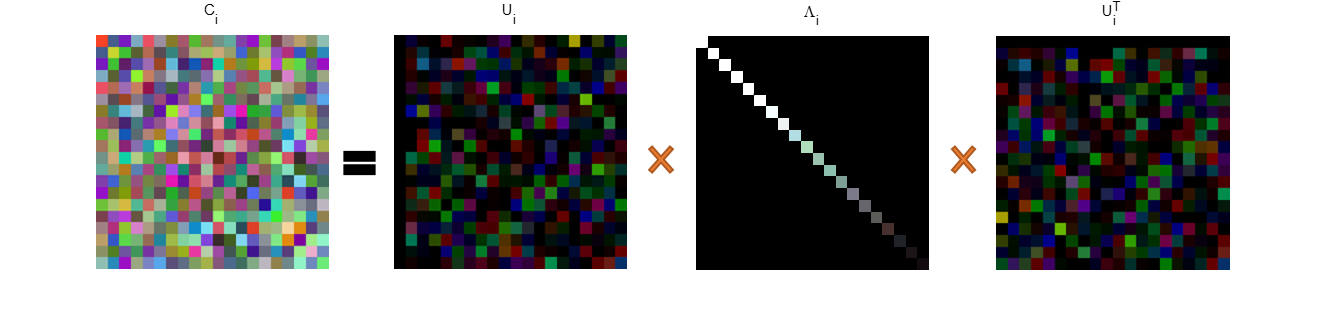
\includegraphics[width=0.95\linewidth]{source/svd_decomposition.png}
	\caption{奇异值分解示意图}
	\label{fig:SVD_Decomposition}
\end{figure}

接下来内容大致安排如下:首先结合着前期关于固定秩对称半正定矩阵流形的研究,对与低秩对称半正定(Low-Rank symmetric Positive Semi-Definite, Low-Rank PSD)矩阵关系最密切的固定秩对称半正定(Fixed-Rank symmetric Positive Semi-Definite, Fixed-Rank PSD)矩阵流形进行介绍,其中为了介绍Fixed-Rank PSD矩阵流形还会用一些篇幅简要介绍一下Stiefel Manifold和Grassmann Manifold;然后结合着工作\cite{PSD_WACV}针对Fixed-Rank PSD矩阵流形建模图像集合中存在的一些问题以及Low-Rank PSD矩阵表示图像集合的优势提出了Low-Rank PSD矩阵建模图像集合的方法;接着是Low-Rank PSD矩阵图像集合表示下的PSD编码和判别学习方法,最后是实验验证本章所提方法和以及本章内容的总结与展望。

\section{施蒂费尔流形和格拉斯曼流形}
\label{sec:Grassmann_Manifold}
这部分会对对称正定矩阵流形以外的两种流形进行介绍,分别是施蒂费尔(Stiefel)流形和格拉斯曼(Grassmann)流形,这里之所以同时介绍这两种流形主要是出于以下考虑:其一是因为Grassmann与Stiefel流形的关系密切使得两者需要同时介绍,其二是为Fixed-Rank PSD流形的介绍做准备。本节的内容只是对Stiefel流形和Grassmann流形的简要介绍,更多关于Grassmann流形以及两者的关系的内容可以参看文献\cite{Grassmann}。以下的内容以基本定义居多,但相较于\ref{sec:Manifold_SPD}节的内容这里的内容相对简单一些;接下来就首先从Grassmann流形的定义开始。
\begin{definition}
\label{Grassmann_def}
{\heiti (\textbf{Grassmann}流形)}Grassmann流形是定义在$\mathbb{R}^n$中所有$k$维的线性子空间构成的集合上的数学结构。
\begin{equation}
{\rm Gr}(k,n)=\{\mathbb{V} \subset \mathbb{R}^n,\mathbb{V}\text{ is a linear subspace with }\rm{dim}\mathbb{V}=k\}
\end{equation}
\end{definition}
当为其定义拓扑结构之后,即可构成流形结构,进一步的可以在其上导出黎曼度量\cite{Grassmann},所以它是黎曼流形的特例。我们最终希望借助Grassmann流形和对称正定矩阵流形来表示固定秩对称半正定矩阵流形,为此需要了解Grassmann流形的数学表示,而Grassmann流形的表示又借助于Stiefel流形,所以出于数学表示的方便性的考虑,这里先对Stiefel流形进行介绍。
\begin{definition}
\label{Stiefel_nonCompact_def}
{\heiti (\textbf{Stiefel(non-compact)}流形)} non-compact Stiefel流形\footnote{以下所说的流形均指集合上定义了拓扑结构的流形,为简洁起见文中仅以集合代替,而不细说拓扑结构}是定义在所有$n\times k,(0<k<n)$满秩矩阵构成的集合上的流形结构。
\begin{equation}
\begin{split}
{\rm St}(k,n)&=\{A \in \mathbb{R}^{n\times k};{\rm rank}(A)=k\}\\
&=\{A=(a_1,...,a_k)\in \mathbb{R}^{n\times k}; a_1,...,a_k \text{ are linearly independent}\}
\end{split}
\end{equation}
\end{definition}
\begin{definition}
\label{Stiefel_Compact_def}
{\heiti (\textbf{Stiefel(compact)}流形)}当在non-compact Stiefel流形\footnotemark[\value{footnote}]的定义域中要求$A$的列向量是正交的(即:$A^{T}A=I_k$)时候,即构成了compact Stiefel流形定义的集合。
\begin{equation}
{\rm St}^{*}(k,n)=\{A\in\mathbb{R}^{n\times k};A^{T}A=I_k\}
\end{equation}
\end{definition}
这里再给出一个在数学中非常重要的概念:“广义线性群(General Linear Group, GL)”,在矩阵流形的研究中将常常见到它的身影。
\begin{definition}
\label{General_Linear_Group}
{\heiti (广义线性群(\textbf{General Linear Group}))}在数学中对于指定的$n$将所有$n\times n$的可逆矩阵的集合称为广义线性群,并记为:
\begin{equation}
{\rm GL}(n)=\{A \in \mathbb{R}^{n\times n};{\rm{det}}(A)\neq 0\}
\end{equation}
\end{definition}

至此,介绍Grassmann流形的准备工作已基本完成,接下来将利用这些定义以及\ref{sec:manifold_Riemaniann}节的内容对Grassmann流形的数学表示进行介绍。为此这里先来捋一捋Grassmann流形和Stiefel流形的关系:
\begin{rela}
\label{Relation_SS}
{\heiti (\textbf{Stiefel(non-compact) V.S Stiefel(compact)})}定义${\rm GS}(\cdot)$表示Gram-Schmidt正交化变换,于是\begin{equation}
{\rm GS}:{\rm St}(k,n) \rightarrow {\rm St}^{*}(k,n)
\end{equation}
\end{rela}
显然${\rm GS}(\cdot)$变换是满射但是不是入射所以${\rm GS}(\cdot)$不是一一的映射。
\begin{rela}
\label{psd_map_pi}
{\heiti (\textbf{Stiefel(non-compact) V.S Grassmann})}定义如公式\ref{noncSt2Gr}所示的变换$\pi$描述两者之间的关系。
\begin{equation}
\label{noncSt2Gr}
\pi:{\rm St}(k,n) \rightarrow {\rm Gr}(k,n),A=(a_1,...a_k)\rightarrow {\rm{span}}(A)
\end{equation}
\end{rela}
同样的$\pi$只是满射但是不是入射,关于映射$\pi$的还有一些性质需要了解:
\begin{itemize}
\item 首先已知$\pi$是满射,对于任意的矩阵$A \in St(k,n)$有
\begin{equation}
\pi^{-1}[\pi(A)]=\{AP;P\in {\rm GL}(k)\}
\end{equation}
\item 映射$\pi$是连续(continuous)的开(open)的(开(open)的意思是说映射的像是开集的话原像也是开集)
\end{itemize}
\begin{rela}
{\heiti (\textbf{Stiefel(compact) V.S Grassmann})}类似于关系\ref{psd_map_pi},定义Stiefel(compact) 和 Grassmann之间的映射$\bar{\pi}$\ref{cSt2Gr}。
\begin{equation}
\label{cSt2Gr}
\bar{\pi}:{\rm St}^{*}(k,n)\rightarrow {\rm Gr}(k,n);A=(a_1,...,a_k)\rightarrow {\rm{span}}(A),A^{T}A=I_k 
\end{equation}
\end{rela}
不难发现映射$\bar{\pi}$与$\pi$之间存在如下的关系:$\pi=\bar{\pi}\circ {\rm GS}$。

前面给出了诸多定义和关系,其目的主要是为了给出Grassmann流形的一个数学表示,方便对其进行研究和应用。
\begin{repr}
\label{non-compact-repr}
利用non-compact Stiefel流形将Grassmann流形表示为如下的商空间(quotient space)的形式
\begin{equation}
St(k,n)/GL(k,\mathbb{R})=\{[A]|[A]\triangleq A[GL(k)];A\in St(k,n)\}
\end{equation}
\end{repr}
\begin{repr}
\label{compact-repr}
Grassmann流形也可利用商空间的概念使用compact Stiefel流形表示:
\begin{equation}
\begin{split}
{\rm St}^{*}(k,n)/{\mathcal{O}}(k)&=\{[A]|[A]\triangleq A[\mathcal{O}(k)];A\in {\rm St}^{*}(k,n\}\\
\mathcal{O}(k)&=\{U|U\in \mathbb{R}^{k\times k};U^{T}U=I_k\}
\end{split}
\end{equation}
\end{repr}
在两种表示中,第二种表示方法更为常用,对该表示的研究也相对成熟一些。在这一小节的最后将介绍Grassmann流形上的度量表示。为此来先介绍两个基本概念:“主夹角”和“投影变换”。
\begin{definition}
\label{Principle_Angle}
{\heiti (主夹角)}假定$X_1,X_2,\in {\rm St}^{*}(k,\mathbb{R}^{n})$表示两个子空间的基矩阵,定义子空间$V_1={\rm{span}}(X_1),V_2={\rm{span}}(X_2)$之间的主夹角为:
\begin{equation}
\begin{split}
\cos\theta_i&=\max_{\bm{u}_i\in V_1}\max_{\bm{v}_i \in V_2}\bm{u}_{i}^{T}\bm{v}_i\\
s.t~~~~& \bm{u}_{i}^{T}\bm{u}_i=1,\bm{v}_{i}^{T}\bm{v}_i=1\\
~~~& \bm{u}_{i}^{T}\bm{u}_j=0,\bm{v}_{i}^{T}\bm{v}_j=0;j \leq i
\end{split}
\end{equation}
其中的$\theta_i,i=1,2,...,k$称为主夹角。
\end{definition}
\begin{definition}
\label{Projection}
{\heiti (投影变换)}在$\mathbb{R}^{n}$空间中,设$S_k$是其中的一个子空间,并且$U$是子空间中的基矩阵($n \times k$),则$\mathbb{R}^{n}$到$S_k$中的投影算子表示如\ref{Projection_Operator}所示。
\begin{equation}
\label{Projection_Operator}
\Pi_k:U\rightarrow UU^{T};U \in {\rm St}^*(k,\mathbb{R}^n)\text{ and }UU^{T} \in \mathbb{S}_n
\end{equation}
\end{definition}
其中$\mathbb{S}_n$表示的是对称矩阵构成的空间。实际上,投影矩阵$UU^{T}$是半正定的。利用“主夹角”和“投影变换”两个概念可方便的介绍Grassmann流形上两个常用的度量的:“投影度量”和“比奈-柯西度量”
\begin{definition}
\label{Projection_metric}
{\heiti (投影度量)}假定$X_1,X_2,\in {\rm St}^{*}(k,\mathbb{R}^{n})$表示两个子空间的基矩阵,并且有主夹角$\{\theta_i\}_{i=1}^{k}$,两者之间定义投影距离度量的定义如\ref{proj_dist}所示。
\begin{equation}
\label{proj_dist}
d(X_1,X_2)=\|\Pi_k(X_1)-\Pi_k(X_2)\|_{2}=\left(\sum_{i=1}^{k}\sin^{2}(\theta_i)\right)^{\frac{1}{2}}
\end{equation}
\end{definition}
其中的$\Pi_k(\cdot)$就是前面的投影变换,这也是“投影度量”的由来。
\begin{definition}
\label{BC_metric}
{\heiti (比奈-柯西度量)}利用主夹角的cosine值$\{\cos(\theta_i)\}_{i=1}^{k}$将该度量定义如下:
\begin{equation}
d(X_1,X_2)=\left(1-\Pi_{i=1}^{k}\cos^{2}(\theta_i)\right)^{1/2}
\end{equation}
\end{definition}
以上是本文关于Grassmann流形的简要介绍,更多关于Grassmann流形的内容可以参看文献\cite{Grassmann},里面有更加详细的介绍,但是可能会比较晦涩。
\section{固定秩对称半正定矩阵流形}
\label{sec:Fixed-rank-PSD}
本文用$\mathbb{S}_{d}^{+}(k)$表示$d \times d$秩为$k$的半正定矩阵组成的集合,它也是我们前期的主要研究对象。接下来将会对固定秩的对称半正定矩阵(Low-Rank symmetric Positive Semi-Definite, PSD)流形的Geomentry结构做简要的介绍,主要内容参考\cite{PSD_Riemannian}。

对于任意的元素$A \in \mathbb{S}_{d}^{+}(k)$将其分解为$A=UR^2U^{T},U\in St^{*}(k,d),R \in \mathbb{S}_{k}^{+}$则这里给出如公式\ref{psd_svd}所示的形式。
\begin{equation}
\label{psd_svd}
A=UR^2U^{T}=(UR)(UR)^{T} \triangleq ZZ^{T};Z \in {\rm St}(k,d)
\end{equation}
这里注意到对任意的正交阵$O \in \mathcal{O}(k)$有$(ZO)(ZO)^{T}=ZZ^{T}$表示的是同一个半正定矩阵因此定义如下的关系:
\begin{equation}
\label{map_by_ortho}
\begin{split}
&R \sim O^{T}RO \in \mathbb{S}^{+}_{k}\\
&U \sim UO \in {\rm St}^{*}(k,d)\\
&ZO=URO \sim UOO^{T}RO
\end{split}
\end{equation}
其中$\sim$表示等价关系,最后定义如下的直积的形式来表示对称半正定的矩阵。
\begin{equation}
\label{psd_product}
(U,R^2)\sim (UO,O^{T}R^2O) \in {\rm St}^*(k,d)\times \mathbb{S}^{+}_{k}
\end{equation}
运用上述公式的内容来表示固定秩半正定矩阵$A$的时候,在其切空间$T_A\mathbb{S}_{d}^{+}(k)$处的无穷小变量$(\Delta,D)$定义为(具体形式可参看文献\cite{PSD_Riemannian}):
\begin{equation}
\label{psd_varation}
\begin{split}
&\Delta=U_{\perp}B,\\
&D=RD_{0}R,\\
\end{split}
\end{equation}
其中$U_{\perp} \in {\rm St}^{*}(d-k,d),U^{T}U_{\perp}=\bm{0};B \in R^{(d-k)\times d}$,而$D_0 \in \mathbb{S}_d$。有了以上的定义后,进一步参考${\rm St}^{*}(k,d)$和$\mathbb{S}^{+}_{k}$上的黎曼度量定义两个微小变量之间的关系\ref{psd_riemannian_metric}。
\begin{equation}
\label{psd_riemannian_metric}
\begin{split}
&g_{(U,R2)}((\Delta_1,D_1), (\Delta_2,D_2)) \\
&~~~~~~~~= {\rm tr}(\Delta_1\Delta_2)+ \lambda~{\rm tr}(R^{−1}D_1R^{−2}D_2R^{−1}),\lambda>0
\end{split}
\end{equation}
可以证明,上式定义了切空间$T_A\mathbb{S}_{d}^{+}(k)$上的黎曼度量\cite{PSD_Riemannian}。公式\ref{psd_curve}利用固定秩对称半正定矩阵中的黎曼度量公式\ref{psd_riemannian_metric}定义了固定秩对称半正定矩阵A,B之间的一条曲线。
\begin{equation}
\label{psd_curve}
\left\{
\begin{aligned}
&let:A\sim(U_A,R_{A}^{2}),B\sim(U_B,R_{B}^{2})\\
&PA\text{ of }U_A,U_B:\Theta={\rm diag}(\theta_1,\theta_2,...,\theta_k)\\
&part1:U(t)=U_A\cos(\Theta t)+X\sin(\Theta t)\\
&part2:R^2(t)=R_{A}\exp\left(t\log\left(R_{A}^{-1}R_{B}^{2}R_{A}^{-1}\right)\right)R_{A}\\
&curve:\gamma_{A \rightarrow B}(t)=U(t)R^{2}(t)U(t)^{T}\\
&length:L(\gamma_{A \rightarrow B})=\|\Theta\|_{F}^{2}+p~\|\log\left(R_{A}^{-1}R_{B}^{2}R_{A}^{-1}\right)\|_{F}^{2}
\end{aligned}
\right.
\end{equation}
公式\ref{psd_curve}中的$PA$是Principle Angles的缩写;$X=(I-U_AU_{A}^{T})U_BF$,其中$F$是矩阵${\rm diag}(\sin(\theta_1),\sin(\theta_2),...,\sin(\theta_k))$的逆(或伪逆);而上式中的$L(\gamma_{A \rightarrow B})$给出了曲线之间的长度,根据定义\ref{Length}如果要进一步的给出流形上的测地距离则需要找到链接$A,B$所有曲线中长度最小的曲线$\gamma_{A \rightarrow B}^{*}(t)$,这对于固定秩的对称正定矩阵流形过复杂,不过好在文献\cite{PSD_Riemannian}证明的了$L(\gamma_{A \rightarrow B})$是测地距离的一个不错估计(虽然它不一定满足三角不等式),所以接下来就可以运用该“度量”。
\begin{equation}
\label{polar_metric}
\delta^{2}_{FRPSD}(A,B)=\|\Theta\|_{F}^{2}+p~\|\log\left(R_{A}^{-1}R_{B}^{2}R_{A}^{-1}\right)\|_{F}^{2}
\end{equation}
\section{固定秩对称半正定矩阵流形研究概况}
\label{sec:Fixed-Rank-PSD-Current}
本节的主要内容是介绍固定秩对称半正定(Fixed-Rank symmetric Positive Semi-Definite, Fixed-Rank PSD)矩阵流形上的判别学习方法。关于对称半正定矩阵(symmetric Positive Semi-Definite, PSD)的研究主要分为如下几个方向:比较纯粹的理论研究(如工作\cite{PSD_Riemannian,PSD_Regression}等),然后是做优化的(如半正定规划问题)研究(如工作\cite{PSD_Opt1}),再者是做度量学习的工作(如AAAI'2016的工作\cite{PSD_AAAI}),最后是做图像集合分类的工作,目前据我们所知只有发表在“Winter Conference on Applications of Computer Vision (WACV), 2016”的工作\cite{PSD_WACV},由于该工作与我们前期的研究内容非常相近并考虑到其前瞻性,接下来将简单的介绍一下,顺带介绍一下Fixed-Rank PSD流形做图像集合分类的这个分支。而其它的分支,如基础理论的已经在\ref{sec:Fixed-rank-PSD}部分做了介绍,优化与度量学习的分支将会在对工作\cite{PSD_AAAI}进行介绍的时候提及,所以这里不再赘述了,接下来就先看一下工作\cite{PSD_WACV}。

工作\cite{PSD_WACV}针对本章开头部分提到的问题,首次利用Fixed-Rank PSD矩阵建模图像集合,用于图像集合的分类问题。文中所提出的方法十分直接,遵循了解决图像集合分类问题的两个基本步骤:1.为图像集合寻找一种表示(这里选择的就是Fixed-Rank PSD矩阵);2.为这种表示寻找/推导一种度量用于描述两个集合表示的相似度/距离。
\subsection{固定秩对称半正定矩阵表示图像集合}
\label{sec:Fixed_Rank_PSD_repr_Imageset}
首先,不妨假设数据包含$n$个图像集合分别属于$C$个类别,并使用标签$y_{i}\in\{1,2,\cdots,C\},i=1,2,\cdots,n$标记(label)。每个集合有$n_i$个样本,每个样本来自$\mathbb{R}^{d}$的空间,于是将由图像集合构造Fixed-Rank PSD矩阵表示的过程描述如下(设${\rm rank}=k$):
\begin{itemize}
\label{construct_fixed_rank_PSD}
\item 设$\{\bm{x}_{ij} \in \mathbb{R}^{d}\}_{j=1}^{n_i}$表示第$i$个图像集合
\item 计算样本均值:$\bar{\bm{x}}_i=\frac{1}{n_i}\sum_{i=1}^{n_i} \bm{x}_{ij}$,样本协方差:$C_i=\frac{1}{n_i-1}\sum_{j=1}^{n_i}(\bm{x}_{ij}-\bar{\bm{x}}_i)(\bm{x}_{ij}-\bar{\bm{x}}_i)^{T}$
\item 对样本协方差矩阵做奇异值分解获得:$C_i=U_i\Lambda_iU_{i}^{T}$,并假设分解结果按特征值由大到小排列
\item 对于给定的${\rm rank}=k$,选取$U_i$的前$k$列$Y_i=U_i(:,1:k)\in {\rm St}^{*}(d,k)$以及$\Lambda_i$的$k$阶主子式$R_{i}^{2}=\Lambda_{i}(1:k,1:k)\in \mathbb{S}_{k}^{+}$作为图像集合的Fixed-Rank PSD表示$(Y_i,R_{i}^{2})$,关于该表示具体可参看本文的\ref{sec:Fixed-rank-PSD}或参考文献\cite{PSD_Riemannian}
\end{itemize}
通过上述的步骤为每一个图像集合构造Fixed-Rank PSD矩阵的表示,为了方便理解这里使用图\ref{fig:FRPSD}对Fixed-Rank PSD进行示意,而关于奇异值分解的示意则可参看图\ref{fig:SVD_Decomposition}。
\begin{figure}[hbt]
	\centering
	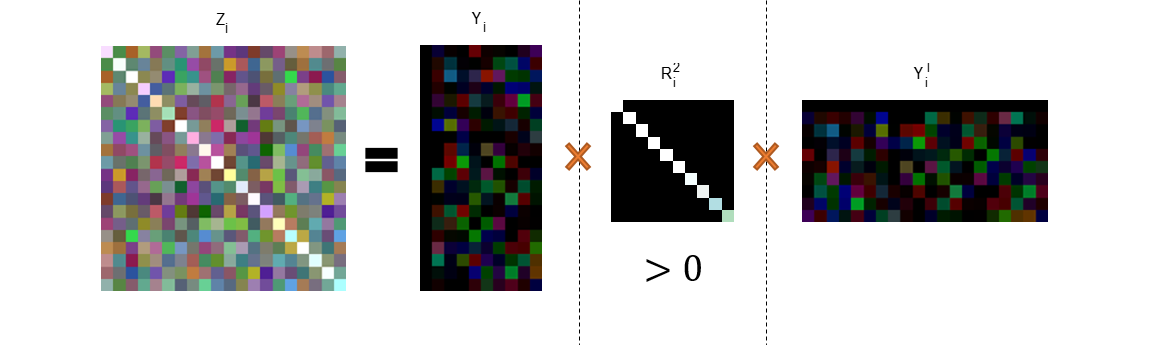
\includegraphics[width=\linewidth]{source/FRPSD.png}
	\caption{固定秩对称半正定矩阵示意图}
	\label{fig:FRPSD}
\end{figure}\\
接下来的部分将借助这种表示对图像集合的分类问题做进一步的探索。
\subsection{固定秩对称半正定矩阵流形用于图像集合分类}
\label{sec:Fixed-Rank-PSD-ImageSet-Start}
在\ref{sec:Fixed_Rank_PSD_repr_Imageset}一节根据\cite{PSD_Riemannian}中介绍的Fixed-Rank PSD矩阵流形的geometry结构对图像集合$i$使用了$(Y_i,R_{i}^{2})\in Gr(n,k)\times \mathbb{S}_{d}^{+}$的表示,使用该表示并运用公式\ref{polar_metric}定义的$\delta_{FRPSD}(\cdot,\cdot)$即可进行图像集合的分类问题了,但是这样的分类方式过于粗糙,没有包含判别性、large margin等一些性质,不利于模型的推广(文献\cite{PSD_WACV}),所以参考\cite{Subspace_GDA,Statistics_CDL}等工作以及工作\cite{Kernel_Riemannian,Dictionary_Extrinsic_method}关于黎曼流形上正定核的结论,也可以为Fixed-Rank PSD矩阵流形定义正定的核的形式来克服以上提到的问题。

关于Fixed-Rank PSD流形上(假设${\rm rank}=k$)的$\delta_{FRPSD}(\cdot,\cdot)$(公式\ref{polar_metric})这里还有一些事实需要注意(为了阐述的方便这里将公式\ref{psd_riemannian_metric}和公式\ref{polar_metric}糅合在一起后用不同的颜色标出前后两部分):
\begin{equation}
\label{polar_metric_split}
\left\{
\begin{aligned}
&g_{(U,R^2)}((\Delta_1,D_1), (\Delta_2,D_2)) \\
&~~~~~~~~~~~={\color{blue}\boxed{{\rm tr}(\Delta_1\Delta_2)}}+ \lambda~{\color{green}\boxed{{\rm tr}(R^{−1}D_1R^{−2}D_2R^{−1})}},\lambda>0\\
&\delta^2(A,B)={\color{blue}\boxed{\|\Theta\|_{F}^{2}}}+\lambda~{\color{green}\boxed{\|\log\left(R_{A}^{-1}R_{B}^{2}R_{A}^{-1}\right)\|_{F}^{2}}}
\end{aligned}
\right.
\end{equation}

其中$\Delta_i,D_i,i=1,2;R_A,R_B,\Theta$的定义请参看\ref{sec:Fixed-rank-PSD}部分的介绍;对于公式\ref{polar_metric_split},注意到其前半部分实际上是Grassmann流形的测地距离,而它与\ref{sec:Grassmann_Manifold}部分介绍的投影度量(Projection Metric,公式\ref{proj_dist})之间仅相差一个倍数关系\cite{PSD_WACV},所以公式\ref{polar_metric_split}的前半部分可以由投影度量来代替,对于公式\ref{polar_metric_split}的后半部分,注意到这是SPD矩阵流形的AIM\cite{AIM_metric}度量,进一步的注意到$R_A,R_B$都是对角矩阵,于是可以得到:$\|\log\left(R_{A}^{-1}R_{B}^{2}R_{A}^{-1}\right)=2\|\log(R_A)-\log(R_B)\|$。综合以上两点特点$\delta^{2}(A,B)$可以进一步的形式化为:
\begin{equation}
\label{polar_metric_kernel}
\begin{split}
\delta^{2}_{FRPSD}(A,B)&=\|Y_{A}Y_{A}^{T}-Y_{B}Y_{B}^{T}\|^{2}_{F}+\lambda\|\log(R_{A})-\log(R_{B})\|^{2}_{F},\lambda>0\\
&=2k-2\|Y_{A}^{T}Y_{B}\|^{2}_{F}+\lambda\|\log(R_{A})-\log(R_{B})\|^{2}_{F}\\
\end{split}
\end{equation}
其中$Y_A,Y_B$的定义在\ref{construct_fixed_rank_PSD}部分已经给出,公式\ref{polar_metric_kernel}中定义的距离很容易证明在$\mathbb{S}^{+}_{d}(k)$上对所有的$\lambda>0$它都是负定的\cite{PSD_WACV},因此容易从\ref{polar_metric_kernel}出发构造正定的核,表格\ref{tab:psd_kernel_list}列出了文章\cite{PSD_WACV}中使用的核。
\begin{table}[htb]
  \centering
  \begin{minipage}[t]{0.8\linewidth} % 如果想在表格中使用脚注,minipage是个不错的办法
  \caption{固定秩对称半正定矩阵流形中的核}
  \label{tab:psd_kernel_list}
    \begin{tabular*}{\linewidth}{lp{10cm}}
      \toprule[1.5pt]
      {\heiti 名称} & {\heiti 形式化} \\\midrule[1pt]
      线性核 & $k_{l}(A,B)=\|Y_{A}^{T}Y_{B}\|_{F}^{2}+\lambda{\rm tr}(\log(R_A)\log(R_B))$\\
      多项式核 & $k_{p}(A,B)=\left(\beta+\|Y_{A}^{T}Y_{B}\|_{F}^{2}+\lambda{\rm tr}(\log(R_A)\log(R_B))\right)^{\alpha}$\\
      拉普拉斯核 & $k_{L}(A,B)=\exp\left(-\beta\sqrt{\lambda\|\log(R_A)-\log(R_B)\|_{F}^{2}-2\|Y_{A}^{T}Y_{B}\|_{F}^{2}}\right)$\\
      RBF核 & $k_{R}(A,B)=\exp\left(-\beta\left(\lambda\|\log(R_A)-\log(R_B)\|_{F}^{2}-2\|Y_{A}^{T}Y_{B}\|_{F}^{2}\right)\right)$\\
      \bottomrule[1.5pt]
    \end{tabular*}
  \end{minipage}
\end{table}\\
最后工作\cite{PSD_WACV}中还对比了经过核判别学习(Kernel Discriminant Analysis, KDA)与不经过KDA学习利用最近邻分类的结果;文章最终的实验在手势识别,视频人脸识别和动态纹理识别进行了验证,关于实验的细节以及结果可以从文章\cite{PSD_WACV}获得,在本章的实验部分也将对这个方法作进一步的讨论。
\section{低秩对称半正定矩阵判别学习方法}
\label{sec:Low-Rank-PSD-Discrim-Approch}
\ref{sec:Fixed-Rank-PSD-ImageSet-Start}小节结合着我们前期的一些尝试介绍了Fixed-Rank PSD矩阵流形用于图像集合分类的工作\cite{PSD_WACV};但是研究中我们发现如下问题:1)通过特征分解获得Fixed-Rank PSD表示的方法\ref{construct_fixed_rank_PSD}比较粗暴,没有考虑其它的信息(如label)的利用;2)虽然工作\cite{PSD_Riemannian}中对$\delta_{FRPSD}(\cdot,\cdot)$(公式\ref{polar_metric})的形式化过程进行了详细的推导,但是$\delta_{FRPSD}(\cdot,\cdot)$本身割裂了$Y_A,R_A$(Grassmann流形和SPD矩阵流形)之间的联系,更切确的说是$\delta_{FRPSD}(\cdot,\cdot)$仅仅借助一个平衡因子$\lambda$很难完全刻画Fixed-Rank PSD矩阵$C_A=Y_{A}R_{A}^{2}Y_{A}^{T}$的关系。

针对上述的一些问题本节给出了我们的改进方案,最后关于方法的验证会在实验部分给出;这里首先要介绍的是如何为每个图像集合构造更具判别力的PSD矩阵表示。

在Mu Yadong发表在的AAAI'16的文章\cite{PSD_AAAI}中,为了在度量学习(Metric Learning, ML)的学习过程中保证马氏距离中的度量矩阵$M$是固定秩对称半正定的以及为了加速算法,文章在固定秩的矩阵流形上提出了一种新的二阶黎曼Retraction算子\footnote{关于Retraction算子读者可以参考本文的第二章}(Second Order Riemannian Retraction Operator)。文中作者构造性的使用$Z_{i}=W_iW_{i}^{T},W_{i}=\left((C_{i}^{1/2}+Z) Y_{i}\right),Y_{i}=U_{i}(:,1:k)$构造PSD矩阵,其中$C_{i},U_{i},Y_{i}$的定义同\ref{construct_fixed_rank_PSD}部分的定义,$Z$是未知的参数,文章\cite{PSD_AAAI}通过要求$Z$满足Fixed-Rank PSD矩阵流形的切空间中的性质来获得一个好的表示,详细内容可以参看文献\cite{PSD_AAAI}。这启示我们在PSD矩阵编码图像集合的时候可以借鉴这种形式,并通过$Z$编码更多的信息,如样本的label信息。

另一方面,前面已经指出$\delta_{FRPSD}(\cdot,\cdot)$(公式\ref{polar_metric})虽然保持了很好geometry相关的性质,但是其分离的形式使得其无法很好的刻画$Y_{i}\in {\rm Gr}(n,k),R_{i} \in \mathbb{S}_{k}^{+}$之间的联系,所以需要寻找一种新的度量形式来刻画两个对称半正定矩阵之间的相似度/距离。为此,如同文章\cite{PSD_Riemannian}一样,考虑到对称半正定矩阵与对称正定矩阵之间的关联性,这里先来回顾一下对称正定矩阵流形中的不同距离度量,并期望从中获得解决方案。
\begin{table}[htb]
	\centering
	\caption{对称正定矩阵流形上的距离度量}
	\begin{tabular}{llcc}
	\toprule[1.5pt]
		{\heiti 距离度量} &{\heiti 形式化} &{\heiti 是测地距离} &{\heiti 可接受不满秩输入}\\ \hline
		Affine-Invariant度量\cite{AIM_metric} &$\|\log(X_{i}^{-\frac{1}{2}}X_jX_{i}^{-\frac{1}{2}})\|_F$ &$\surd$ &$\times$ \\
		Log-Euclidean度量\cite{LEM_metric} &$\|\log(X_{i})-\log(X_{j})\|_F$ &$\surd$ &$\times$ \\
		Stein散度\cite{Stein_divergence} &$\log{\rm det}(\frac{X_1+X_2}{2})-\frac{1}{2}\log{\rm det}(X_1X_2)$ &$\times$ &$\times$ \\
		Jeffreys散度\cite{Jeffreys_divergence} &$\frac{1}{2}{\rm tr}(X_{1}^{-1}X_2+X_{2}^{-1}X_{1})-d$ &$\times$ &$\times$\\
		Cholesky距离\cite{Cholesky_distance} &$\|chol(X_1)-chol(X_2)\|_{F}$ &$\times$ &$\surd$\\
		Power-Euclidean度量\cite{Cholesky_distance} & $\frac{1}{\alpha}\|X_{1}^{\alpha}-X_{2}^{\alpha}\|_{F}$ &$\times$ &$\surd$\\
	\bottomrule[1.5pt]
	\end{tabular}
	\label{tab:SPD_metric_list}
\end{table}\\
表格\ref{tab:SPD_metric_list}中$chol(\cdot)$表示的是Cholesky分解。

表格\ref{tab:SPD_metric_list}中列出的所有的度量均可用于对称正定矩阵的之间距离的度量,其中Affine-Invariant度量和Log-Euclidean度量分别在\cite{AIM_metric}和\cite{LEM_metric}被提出,且它们有各自的黎曼度量也是是$\mathbb{S}_{d}^{+}$上的测地距离,并且Log-Euclidean度量以其优于Affine-Invariant度量的计算性质而赢得了不少青睐,但是遗憾的是这两种度量都不能用于不满秩(也就是半正定的)的情况,Stein散度\cite{Stein_divergence}和Jeffreys散度\cite{Jeffreys_divergence}最初是为了提高计算效率而提出来的,但是由于Stein散度需要计算$\log {\rm det}(\cdot)$而Jeffreys散度需要计算$X_{i}^{-1},i=1,2$所以也不能直接用于处理半正定的输入,最后剩下Cholesky距离\cite{Cholesky_distance}和Power-Euclidean度量\cite{Cholesky_distance}这两种度量由于不涉及求逆或者$\log(\cdot)$操作所以可以直接用于半正定矩阵,而与$\delta_{FRPSD}(\cdot,\cdot)$(公式\ref{polar_metric})相比,其直接考虑半正定输入,没有割裂${\rm Gr}(d,k),\mathbb{S}_{k}^{+}$之间的关系,应该有更好的表示能力;但需要注意到的是Cholesky距离和Power-Euclidean度量并不是$\mathbb{S}_{d}^{+}$上的测地距离更不是$\mathbb{S}_{d}^{+}(k)$上的测地距离,因此不能完全刻画$\mathbb{S}_{d}^{+}(k)$的geometry的结构,不过本文相信它们的联合的形式的优点能够弥补其不是测地距离的不足(最后的实验验证了我们的观点)。接下来这里选择Cholesky距离和Power-Euclidean度量作为半正定矩阵的度量。特别地,简单的验证试验发现Power-Euclidean度量比Cholesky距离能够更好的刻画数据本身的性质,所以本章接下来的部分以Power-Euclidean度量进行介绍和实验。

最后还需要注意的是文章\cite{PSD_WACV}使用Fixed-Rank PSD建模图像集合的方法中,Fixed-Rank的约束主要是为了能够在PSD上定义流形的geometry结构,并利用该geometry结构进行判别学习;但是在使用Power-Euclidean度量两个PSD矩阵之间的关系的时候Fixed-Rank的性质却不是那么必要,而此时Low-Rank成为更本质的一个要求,因此接下来的内容中我们使用更一般的Low-Rank PSD矩阵建模图像集合。

以上是对本文所提方法的一个概要介绍,下面将进一步细化该方法。遵循图像集合分类问题的两个主要步骤将接下来的内容大致分为:1)如何利构造一个好的Low-Rank PSD的表示;2)如何利用Power-Euclidean度量进行判别学习以及Low-Rank PSD矩阵上的判别学习方法的形式化。
\subsection{融入判别信息的低秩对称半正定矩阵的构造}
\label{sec:discrim_Low_Rank_PSD}
在\ref{sec:Low-Rank-PSD-Discrim-Approch}节的前半部分提出了借鉴\cite{PSD_AAAI}中构造PSD的内容(公式\ref{construct_discriminat_psd}),构造图像集合的带判别性的低秩对称半正定矩阵表示:
\begin{equation}
\label{construct_discriminat_psd}
Z_{i}=W_iW_{i}^{T},W_{i}=\left((C_{i}^{1/2}+Z) Y_{i}\right),Y_{i}=U_{i}(:,1:k),C_i=U_i\Lambda_iU_{i}^{T},R_{i}^{2}=\Lambda
\end{equation}
在这里先简单说明一下这种构造方式的合理性:在$Z_{i}=\left((C_{i}^{1/2}+Z)Y_{i}\right)\left((C_{i}^{1/2}+Z)Y_{i}\right)^{T}$中当$Z=\bm{0}$时,则$Z_{i}$等价于文章\cite{PSD_WACV}中Fixed-Rank PSD矩阵的构造方式:
\begin{equation}
\label{Fixed-Rank-PSD-Z0}
\begin{split}
Z_{i}&=\left((C_{i}^{1/2}+Z)Y_{i}\right)\left((C_{i}^{1/2}+Z)Y_{i}\right)^{T}\\
&=\left((U_{i}R_{i}U_{i}^{T})U_{i}(:,1:k)\right)\left((U_{i}R_{i}U_{i}^{T})U_{i}(:,1:k)\right)^{T}\\
&=\left(U_{i}R_{i}(:,1:k)\right)\left(U_{i}R_{i}(:,1:k)\right)^{T}\\
&=\left(U_{i}(:,1:k)R_{i}^{2}(1:k,1:k)U_{i}(:,1:k)^{T}\right)\\
\end{split}
\end{equation}\\
此外,当$Z=I-C_{i}^{\frac{1}{2}}$时:
\begin{equation}
\label{Fixed-Rank_PSD-Z_neg}
Z_i=Y_{i}Y_{i}^{T}
\end{equation}
正好是\cite{Subspace_GDA}中的投影矩阵的结果,由此可以一定程度上说明\ref{construct_discriminat_psd}构造的合理性。

说明完合理性之后,接下是如何选择公式\ref{construct_discriminat_psd}中的$Z$的问题,虽然文章\cite{PSD_AAAI}中给出了一种构造的方式,但是由于目的不同(文章\cite{PSD_AAAI}中是为了优化马氏距离中的度量矩阵,这里是为了表示图像集合)所以这里选择另一种矩阵$Z$的构造方式:借助判别学习(Discriminate Learning)的框架学习矩阵$Z$,将判别信息编码到图像集合的PSD表示中。

要把判别信息融入到Low-Rank PSD矩阵表示的编码中,一个直接有效的方法就是要求同类的样本更相似而不同类的样本则尽量不相似。为此,利用样本标签$y_{i},i=1,2,\cdots,n$定义两两样本之间的关系矩阵$G\in\{-1,1\}^{n\times n}$,其中$G_{ij}$的定义如下:
\begin{equation}
\label{Realtion_Mat}
G_{ij}=\left\{
\begin{split}
&1,\text{if }y_i=y_j\\
&-1,\text{else}
\end{split}
\right.
\end{equation}
其中$y_i,i=1,2,\cdots,n$表示的是样本的标签。经过简单的变换并利用公式\ref{label_represent}的表示,可以得到$G=2YY^{T}-1$。但是注意到,在实际的判别学习的方法研究中,要求所有的同类样本对的相似度尽量大而不同类样本对的相似度尽量小是不太现实的,而且这样也会增加算法的计算量,所以这里进一步的考虑在Graph Embedding\cite{Graph_Embeding}的框架下构造正负样本对:首先定义两个参数$k_w,k_b$,其意义类似于kNN分类器中的参数$k$,$k_w$描述的是当前样本与同类样本的近邻关系,$k_b$描述的是当前样本与不同类的样本的近邻关系,利用$k_w,k_b$定义$G_w,G_b$:
\begin{equation}
\label{GE_Gw_Gb}
\begin{split}
&G_w=\{G^{w}_{ij}\}_{n \times n},\text{where }G^{w}_{ij}=\left\{
\begin{split}
&1,\text{$j$与$i$同类且属于$i$的$k_w$近邻}\\
&0,\text{否者}
\end{split}
\right.\\
&G_b=\{G^{b}_{ij}\}_{n \times n},where~G^{b}_{ij}=\left\{
\begin{split}
&1,\text{$j$与$i$不同类但属于$i$的$k_b$近邻}\\
&0,\text{否则}
\end{split}
\right.
\end{split}
\end{equation}
最后,利用$G_w,G_b$对公式\ref{Realtion_Mat}中的$G$进行重新定义:
\begin{equation}
\label{Graph_Mat}
G=G_w-G_b
\end{equation}
其意义可用图\ref{fig:Graph_Embedding}表示。
\begin{figure}[hbt]
	\centering
	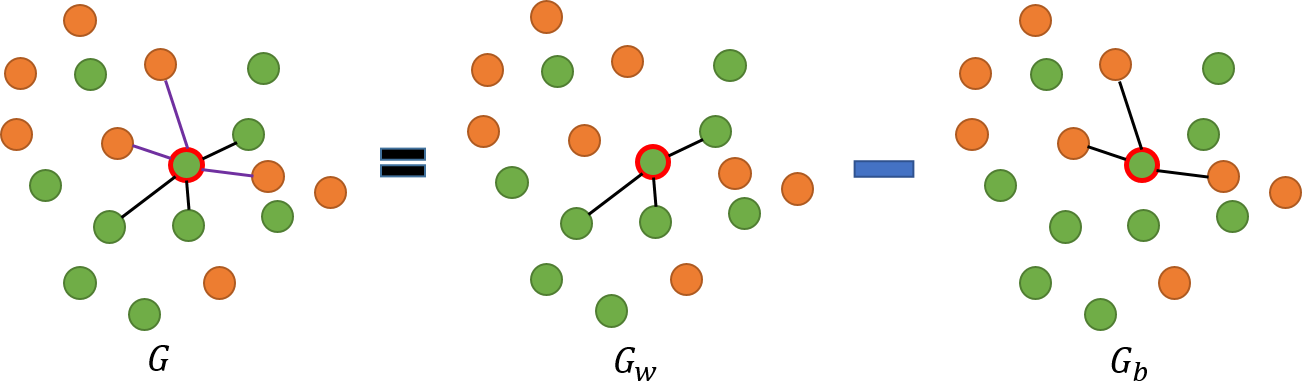
\includegraphics[width=\linewidth]{source/Graph_Embedding.png}
	\caption{图嵌入框架示意图}
	\label{fig:Graph_Embedding}
\end{figure}
此外,为了平衡正负样本对的比例,实验中还将$G$中的$1,-1$分别除以正负样本对的个数。

接下来,使用$\rho_{ij}=\frac{\left<Z_{i},Z_{j}\right>_{F}}{\|Z_{i}\|_{F}\|Z_{j}\|_{F}};i,j=1,2,\cdots n$来度量两个表示之间的相似度\footnote{注:这里不使用$\frac{\left<Z_{i}^{\frac{1}{m}},Z_{j}^{\frac{1}{m}}\right>_{F}}{\|Z_{i}\|_{F}^{\frac{1}{m}}\|Z_{j}^{\frac{1}{m}}\|_{F}};i,j=1,2,\cdots n$的原因主要是这会大大增加计算复杂度而且当$n>1$时$x^{\frac{1}{n}}$的导数未定义,所以这里退而求其次};利用$\rho_{ij}$和$G_{ij}$的定义,给出公式\ref{FRPSD_discriminant}中的损失函数:
\begin{equation}
\label{FRPSD_discriminant}
C(Z)=-\sum_{i=1}^{n}\sum_{j=1}^{n}G_{ij}\rho_{ij}^{2}={\rm tr}(GF^{T})+\gamma\|Z\|_{F}^{2},where~F_{ij}=\rho_{ij}^{2}
\end{equation}
其中函数$C(Z)$的最后一项是正则项,其目的是为了防止过拟合,这虽然只是一个小的trick,但是实验中发现该trick却比较有效。

我们的目标是使最终编码的$Z_{i}, i=1,2,\cdots n$让$C(Z)$最小。这是一个矩阵函数的优化问题,为此需要计算目标函数的导数。为了叙述的方便,这里把第二章的两条在计算矩阵方向导数的时候的规律($rule$\ref{devi_rules_2})再表述一遍。
\begin{displaymath}
\label{devi_rules}
\left\{
\begin{split}
&rule~1:D_{X}(f\circ g)(X)[H]=D_{g(X)}f(g(X))[D_{X}g(X)[H]]\\
&rule~2:D_{X}\left<f(X),g(X)\right>[H]=\left<D_{X}f(X)[H],g(X)\right>+\left<f(X),D_{X}g(X)[H]\right>
\end{split}
\right.
\end{displaymath}
关于矩阵函数的方向导数的具体内容,读者可以参看本文第二章的内容,此外读者也可以在\cite{Maniopt_DiscreteCurveFitting}中找到关于$rule~1,rule~2$的内容。

对于最小化问题\ref{FRPSD_discriminant},这里使用共轭梯度算法进行求解,为此需要预先计算$C(Z)$的梯度$\nabla_{Z}C(Z)$,为了方便起见定义$k_{ij}=\left<Z_{i},Z_{j}\right>_{F}$,接下来利用公式\ref{discrimZ_search_gradeint}对$C(Z)$计算其关于$Z$的导数。
\begin{equation}
\label{discrimZ_search_gradeint}
\begin{split}
C(Z)={\rm tr}(GF^{T})+\gamma\|Z\|_{F}^{2}&=\sum_{i=1}^{n}\sum_{j=1}^{n}G_{ij}F_{ij}+\gamma\|Z\|_{F}^{2}=\sum_{i=1}^{n}\sum_{j=1}^{n}G_{ij}\frac{k_{ij}^2}{k_{ii}k_{jj}}+\gamma\|Z\|_{F}^{2}\\
\frac{\partial}{\partial Z}C(Z)&=\sum_{i=1}^{n}\sum_{j=1}^{n}G_{ij}\left(c_1\frac{\partial}{\partial Z}k_{ij}-c_2\frac{\partial}{\partial Z}k_{ii}-c_3\frac{\partial}{\partial Z}k_{jj}\right)+2\gamma Z\\
{\rm where~~}c_1&=\frac{2k_{ij}k_{ii}k_{jj}}{(k_{ii}k_{jj})^2},c_2=\frac{k_{ij}k_{ij}k_{jj}}{(k_{ii}k_{jj})^2},c_3=\frac{k_{ij}k_{ij}k_{ii}}{(k_{ii}k_{jj})^2}
\end{split}
\end{equation}
公式\ref{discrimZ_search_gradeint}中$\frac{\partial}{\partial Z}k_{ij}$的计算与第二章中第一个例子\ref{MatrixFunc_devi_example1}的计算类似,具体过程如下:
\begin{equation}
\label{discrimZ_search_part1_gradeint}
\begin{split}
D_{Z}k_{ij}[H]&=D_{Z}\left<Z_i,Z_j\right>_{F}\\
&=\left<D_{Z}Z_i[H],Z_j\right>_{F}+\left<Z_i,DZ_j[H]\right>_{F}
\end{split}
\end{equation}
由于$\left<D_{Z}Z_i[H],Z_j\right>_{F}$与$\left<Z_i,D_{Z}Z_j[H]\right>_{F}$的计算是类似的,所以仅以前一部分作为研究对象,其结果可以很好的平移到另一部分。
\begin{equation}
\label{discrimZ_search_part2_gradeint}
\begin{split}
\left<D_{Z}Z_i[H],Z_j\right>_{F}&=\left<D_{Z}\left((C_{i}^{\frac{1}{2}}+Z)S_{i}(C_{i}^{\frac{1}{2}}+Z)^{T}\right)[H],(C_{j}^{\frac{1}{2}}+Z)S_{j}(C_{j}^{\frac{1}{2}}+Z)^{T}\right>_{F}\\
D_{Z}\left((C_{i}^{\frac{1}{2}}+Z)S_{i}(C_{i}^{\frac{1}{2}}+Z)^{T}\right)[H]&=D_{Z}(C_{i}^{\frac{1}{2}}S_{i}C_{i}^{\frac{T}{2}}+C_{i}^{\frac{1}{2}}S_{i}Z^{T}+ZS_{i}C_{i}^{\frac{T}{2}}+ZS_{i}Z^{T})[H]\\
&=C_{i}^{\frac{1}{2}}S_{i}H^{T}+HS_{i}C_{i}^{\frac{T}{2}}+HS_{i}Z^{T}+ZS_{i}H^{T}\\
&=(C_{i}^{\frac{1}{2}}+Z)S_{i}H^{T}+HS_{i}(C_{i}^{\frac{T}{2}}+Z^{T})
\end{split}
\end{equation}
其中$S_{i}=Y_{i}Y_{i}^{T},i=1,2,\cdots,n$,接下来利用公式\ref{discrimZ_search_part2_gradeint}的结果,得到公式\ref{discrimZ_gradient}的结果(其中利用了$Z_{i},S_{i};i=1,2,\cdots,n$是对称矩阵的结果)。
\begin{equation}
\label{discrimZ_gradient}
\left\{
\begin{split}
\left<D_{Z}Z_i[H],Z_j\right>_{F}&=\left<(C_{i}^{\frac{1}{2}}+Z)S_{i}H^{T}+HS_{i}(C_{i}^{\frac{T}{2}}+Z^{T}),Z_j\right>_{F}\\
&={\rm tr}\left((C_{i}^{\frac{1}{2}}+Z)S_{i}H^{T}Z_j\right)+{\rm tr}\left(HS_{i}(C_{i}^{\frac{T}{2}}+Z^{T})Z_j\right)\\
&={\rm tr}\left(H^{T}Z_j(C_{i}^{\frac{1}{2}}+Z)S_{i}\right)+{\rm tr}\left(HS_{i}(C_{i}^{\frac{T}{2}}+Z^{T})Z_j\right)\\
&=2{\rm tr}\left(H^{T}Z_j(C_{i}^{\frac{1}{2}}+Z)S_{i}\right)=2\left<H,Z_j(C_{i}^{\frac{1}{2}}+Z)S_{i}\right>_{F}\\
D_{Z}k_{ij}[H]&=2\left<H,Z_j(C_{i}^{\frac{1}{2}}+Z)S_{i}\right>_{F}+2\left<H,Z_i(C_{j}^{\frac{1}{2}}+Z)S_{j}\right>_{F}\\
\frac{\partial}{\partial Z}k_{ij}&=2Z_j(C_{i}^{\frac{1}{2}}+Z)S_{i}+2Z_i(C_{j}^{\frac{1}{2}}+Z)S_{j}\\
&=2(Z_{j}W_{i}Y_{i}^{T}+Z_{i}W_{j}Y_{j}^{T})
\end{split}
\right.
\end{equation}
最后结合公式\ref{discrimZ_search_gradeint}和\ref{discrimZ_gradient}的结果,即可计算出$C(Z)$的梯度,将其作为共轭梯度算法的输入,最小化$C(Z)$获得$Z^{*}$即可用于对图像集合的PSD编码。这里使用图\ref{fig:Discrim_LRPSD}示意带判别信息的低秩对称正定矩阵编码图像集合的模型。
\begin{figure}[htb]
	\centering
	\subcaptionbox{半正定矩阵平方根示意图}
      	{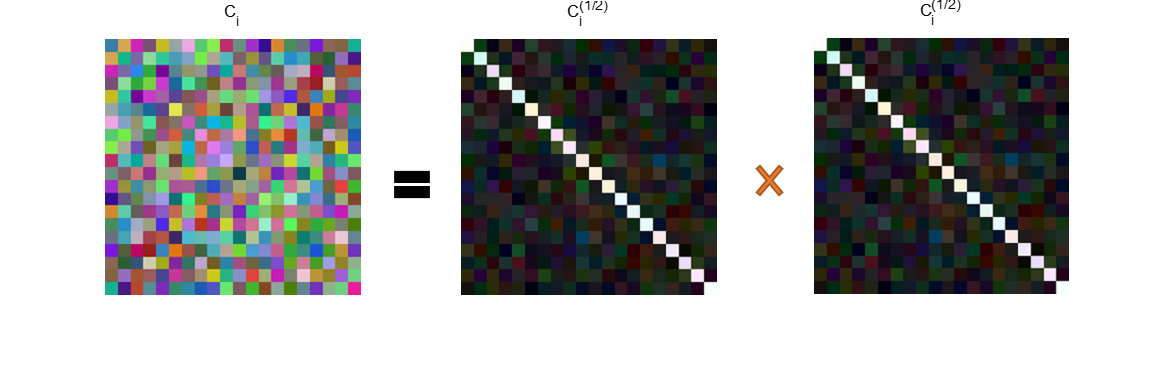
\includegraphics[width=\linewidth]{source/Discrim_LRPSD_sqrt.png}}
	\subcaptionbox{编码判别信息的$W_{i}$的示意图}
		{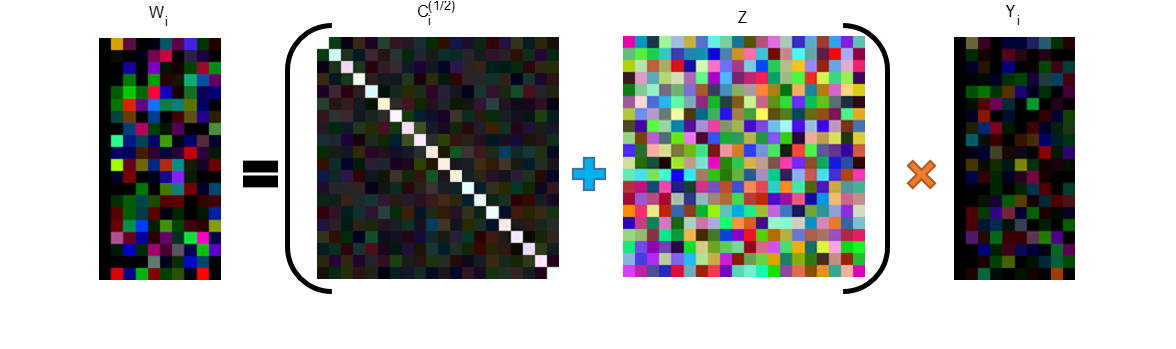
\includegraphics[width=\linewidth]{source/Discrim_LRPSD_W.png}}
	\caption{带判别信息的低秩对称半正定矩阵模型示意图}
	\label{fig:Discrim_LRPSD}
\end{figure}
\subsection{低秩对称半正定矩阵集合上的判别学习方法}
在\ref{sec:discrim_Low_Rank_PSD}小节中介绍了将判别信息编码到Low-Rank PSD矩阵问题,但是仅仅有内嵌入判别性的编码还是不足以处理太复杂的问题,且算法也不具有Large Margin等性质,类似于\cite{PSD_WACV}中的方法,这里选择在核判别学习(Kernel Discriminant Learning, KDA\cite{Kernel_KDA})的框架下进行判别学习。特别地,注意到Power-Euclidean度量的定义可以由$k_{ij}=\left<Z_{i}^{\frac{1}{m}},Z_{j}^{\frac{1}{m}}\right>_{F}$的kernel的形式导出,并且容易证明$K=\{k_{ij}\}_{n\times  n}$的正定性。

由于KDA\cite{Kernel_KDA}的研究已经非常成熟,且这里也不是对它的改进或相关的工作,所以不会从头再介绍一遍,而只会简单的回顾一下KDA的基本思想:首先,KDA的基础是线性判别分析(Linear Discriminant Analysis, LDA),其目标是使得内类散度小而类间散度大。KDA则是LDA在再生核希尔伯特空间(Reproducing Kernel Hilbert space, RKHS)中的版本,其目的与LDA一样。文献\cite{Kernel_KDA}中给出了十分简洁的KDA的形式:设$n_c,c=1,2,\cdots,C$表示各个类别中的样本数,$\sum_{c=1}^{C}n_{c}=n$,这里的$n$表示的是样本总数,$\phi(\cdot)$表示的是非线性变化(例如接下来将要使用的$\phi(Z_{i})=Z_{i}^{\frac{1}{n}},n>1$),定义核矩阵$K=\{k_{ij}\}_{n\times n}$,其中$k_{ij}=\left<\phi(Z_{i}),\phi(Z_j)\right>_{F}$,则KDA的目标形式化为公式\ref{KDA_Formulation}。
\begin{equation}
\label{KDA_Formulation}
\bm{\alpha}_{opt}=\arg \max\frac{\bm{\alpha}^{T}KWK\bm{\alpha}}{\bm{\alpha}^{T}KK\bm{\alpha}}
\end{equation}
其中$W$的定义如公式\ref{KDA_W_def}所示。
\begin{equation}
\label{KDA_W_def}
W=\{W_{ij}\}_{n \times n},\text{where }W_{ij}=\left\{
\begin{split}
&\frac{1}{n_{c}},\text{若$Z_{i},Z_{j}$同时属于第c类}\\
&0, \text{否则}
\end{split}
\right.
\end{equation}
以上便是本章所提方法使用的判别学习方法——KDA\cite{Kernel_KDA}的介绍,试验中我们使用了文献\cite{KDA_DengCai1,KDA_DengCai2}提供的代码。
\section{实验结果与分析}
本章所做的问题是使用Low-Rank PSD矩阵表示集合数据,并在该表示下进行集合数据的分类问题,任务与第二章的任务类似,都是集合数据的分类问题,所以这里使用了相同的数据进行实验(物体识别数据库ETH\cite{Database_ETH80},材质分类数据库UIUC\cite{Database_UIUC}以及视频人脸识别数据库\cite{Database_YTC}),这几个数据库上的实验任务已经在\ref{sec:RPLS_exp}部分做了相对细致的介绍,同时数据库的规模(包含了小数据库ETH,中等规模数据库UIUC,较大规模的数据库YTC)也具有一定的代表性;各个数据集合上的基本特征的提取与\ref{Database_feature}节介绍的方式相同,这里不再赘述;在获得原始特征之后,利用公式\ref{MeanCov_SPD_Construct}构造初始半正定矩阵表示$C_{i}$(此时不需要再加正则项),然后利用\ref{sec:discrim_Low_Rank_PSD}的编码过程获得图像集合带判别性的低秩对称半正定矩阵表示。关于数据库的详细介绍以及对应的测试协议可以参看\ref{sec:data_intro}部分的内容,而关于原始图像特征的提取部分的内容则可以参看\ref{Database_feature}节的内容。最后表\ref{tab:LRPSD_experiment}给出了我们的实验结果。

\begin{table}[htb]
	\centering
	\caption{低秩对称半正定矩阵判别学习方法对比实验结果}
	\begin{tabular*}{\linewidth}{@{\extracolsep{\fill}}|l|ccc|}\hline
		\diagbox{方法}{数据集} &ETH80 &UIUC &YTC \\ \hline
		GDA\cite{Subspace_GDA} &92.50$\pm$3.54	&53.33$\pm$2.32 &66.73$\pm$3.16 \\ \hline
		CDL-PLS\cite{Statistics_CDL} &93.25$\pm$4.72 &53.89$\pm$4.06 &70.28$\pm$2.13 \\ \hline
		RSR-Stein\cite{Dictionary_RSR} &93.25$\pm$3.34 &52.41$\pm$4.03 &72.77$\pm$2.69  \\ \hline
		SPDML-Stein\cite{Statistics_SPDML} &90.50$\pm$3.87 &49.17$\pm$2.37 &61.57$\pm$3.43  \\ \hline
		SPDML-AIM\cite{Statistics_SPDML} &90.75$\pm$3.34 &48.09$\pm$1.82 &64.66$\pm$2.92  \\ \hline
		LEML\cite{Statistics_LEML}&94.75$\pm$2.49 &48.98$\pm$3.69 &70.53$\pm$2.95  \\ \hline
		${\rm FRPSD-KDA}_{Linear}$\cite{PSD_WACV}&94.50$\pm$3.07	&52.04$\pm$3.80	&70.93$\pm$3.28  \\ \hline
		${\rm FRPSD-KDA}_{Polynomial}$\cite{PSD_WACV}&\textbf{96.00$\pm$2.42}	&56.02$\pm$3.93 &70.74$\pm$3.05  \\ \hline
		${\rm FRPSD-KDA}_{Laplace}$\cite{PSD_WACV}&95.50$\pm$2.84 &57.69$\pm$3.35 &70.14$\pm$3.04  \\ \hline
		${\rm FRPSD-KDA}_{RBF}$\cite{PSD_WACV}&95.50$\pm$3.50 &57.78$\pm$4.10 &70.96$\pm$3.05\\ \hline
		${\rm \bm{LRPSD-KDA}}$ &\textbf{93.25$\pm$4.72} &\textbf{59.17$\pm$3.48} &\textbf{74.37$\pm$2.96}  \\ \hline
		${\rm \bm{LRPSD-KDA}}_{discrim}$ &\textbf{94.50$\pm$2.48} &\textbf{59.81$\pm$3.58} &\textbf{74.73$\pm$2.91}  \\ \hline
	\end{tabular*}
	\label{tab:LRPSD_experiment}
\end{table}
其中,${\rm FRPSD-KDA}$是文章\cite{PSD_WACV}中方法的简称(是Fixed-Rank PSD和KDA的缩写),其下标表示了核的类型:线性核($Linear$)、多项式核($Polynomial$)、Laplace核($Laplace$)以及RBF核($RBF$),${\rm LRPSD-KDA}$则表示本章所提的方法的简称(是Low-Rank PSD和KDA的缩写),其中下标$discrim$表示的方法是否使用\ref{sec:discrim_Low_Rank_PSD}部分的编码学习方式构造图像集合的Low-Rank PSD矩阵表示。

表格\ref{tab:LRPSD_experiment}中选取的方法与\ref{sec:RPLS_exp_result_analysis}部分选择方法类似,包含了目前取得state-of-the-art的一些主要方法,此外还包含了与我们最相关的工作\cite{PSD_WACV}中的方法的结果,由于作者没有公布源代码,所以我们小心的实现并进行细致的参数调节之后汇报我们所获得的最好的结果。还有GDA\cite{Subspace_GDA}的结果(该结果也是自己实现并小心调参后获得的结果)。其它方法我们均从作者主页获取代码并小心调参后汇报的最好的结果。

从表格\ref{tab:LRPSD_experiment}我们的可以得到的信息是:本章所提的${\rm \bm{LRPSD-KDA}}$方法在三个数据集上获得了与state-of-the-art可比甚至是更好的性能,相较于子空间和协方差建模的方法(表格\ref{tab:LRPSD_experiment}的前两行),${\rm \bm{LRPSD-KDA}}$方法在三个任务上都有相对明显的提升。我们认为获得这种提升的主要原因有两个方面:1)通过与文章\cite{PSD_WACV}中的方法(表中的${\rm FRPSD-KDA}$一类方法)相比,可得出本文使用的Power-Euclidean度量更能刻画PSD矩阵的性质的结论,这与我们的一开始的想法是吻合的;2)表中的最后六行的结果与其它行的结果相比说明了PSD建模图像集合的有效性。最后还注意到融入判别信息带来提升,虽然幅度不大(这与本文选择的相对简单的融合方式有关)但是可以看出方向的正确性,这里还有上升的空间。

实验中还发现:公式\ref{FRPSD_discriminant}中的正则项$\gamma\|Z\|_{F}^{2}$对结果的影响与数据集相关,对于每个集合中数据较少或噪声较大的数据集,如ETH\cite{Database_ETH80}和YTC\cite{Database_YTC}(其中YTC属于集合个数多,但是每个集合都不是很大的类型,这在视频监控中很常见)该项的设置很重要,但是对于每个集合中样本较多的数据集该项则可忽略掉(如:在UIUC\cite{Database_UIUC}上我们设置$\gamma=0$),其它实验参数的设置主要包含$k_w,k_b$的设置,Power-Euclidean度量中$n$(或$\alpha=\frac{1}{n}$)的设置,以及Low-Rank约束的上界$k$的设置。由于都是整数设置方法比较常规这里就不再一一赘述。最后,需要注意的是利用Power-Euclidean度量还可以定义其它的核的形式,表\ref{tab:PSD_PowerMetric_KernelList}中给出了kernel的形式:
\begin{table}[htb]
  \centering
  \begin{minipage}[t]{0.8\linewidth} % 如果想在表格中使用脚注,minipage是个不错的办法
  \caption{Power-Euclidean度量相关的核}
  \label{tab:PSD_PowerMetric_KernelList}
    \begin{tabular*}{\linewidth}{lp{10cm}}
      \toprule[1.5pt]
      {\heiti 名称} & {\heiti 形式化} \\\midrule[1pt]
      线性核 & $k_{l}(A,B)={\rm tr}\left(Z_{i}^{\frac{1}{m}}Z_{j}^{\frac{T}{m}}\right)$\\
      多项式核 & $k_{p}(A,B)=\left(\beta+{\rm tr}\left(Z_{i}^{\frac{1}{m}}Z_{j}^{\frac{T}{m}}\right)\right)^{\alpha}$\\
      拉普拉斯核 & $k_{L}(A,B)=\exp\left(-\beta\sqrt{\|Z_{i}^{\frac{1}{m}}-Z_{j}^{\frac{T}{m}}\|_{F}^{2}}\right)$\\
      RBF核 & $k_{R}(A,B)=\exp\left(-\beta{\|Z_{i}^{\frac{1}{m}}-Z_{j}^{\frac{T}{m}}\|_{F}^{2}}\right)$\\
      \bottomrule[1.5pt]
    \end{tabular*}
  \end{minipage}
\end{table}

但是从实验结果中可以看出:在线性核下我们已经得到了与state-of-the-art可比甚至是更好一些的结果,此外Kernel的方法的引入虽然会对最终的结果有所提高(部分测试试验中发现Laplace Kernel对于Power-Euclidean度量有更好的促进作用),但是由于引入了更多的参数需要调节,所以使得算法的实际运用价值打了折扣;因此这里仅把kernel的方法作为一个未来深入方向,而不在这里做深入讨论。
\section{总结与下一步工作}
在本章中我们针对集合数据的建模问题以及集合数据特征本身存在的一些问题,使用PSD矩阵建模图像集合,并且结合前期关于Fixed-Rank PSD流形的研究以及工作\cite{PSD_WACV}的内容,针对使用子空间、协方差矩阵以及Fixed-Rank PSD矩阵建模图像集合的工作\cite{PSD_WACV}中存在的问题,提出了Low-Rank PSD矩阵的判别学习方法,主要的内容可以归纳为如下几点:1)使用带有判别性的低秩对称半正定矩阵表示图像集合;2)针对文献\cite{PSD_WACV}中的使用的$\delta_{FRPSD}(\cdot,\cdot)$(公式\ref{polar_metric})割裂了Grassmann流形和对称正定矩阵流形之间关系的问题提出了使用Power-Euclidean度量进行判别学习的方法;3)在KDA\cite{Kernel_KDA}的框架下进行判别学习获得与state-of-the-art可比甚至是更好的结果。

最后,前面已经提到表格\ref{tab:LRPSD_experiment}中的结果显示判别学习与非判别学习的结果提升不是特别的明显,究其原因的话可能是Graph Embedding的框架与最后的KDA的框架没有很好的适配的原因,这里的问题值得深入研究,此外就是前面提到的使用更多Kernel版本的方法,可能也是一个尝试的方向。
% created on 2016-03-39
\chapter{结束语}
\label{chap:The_End}
计算视觉问题的研究经过几十年的发展,取得了巨大的成就。在计算机视觉中,集合数据的研究经历十多年时间也已然成为视觉任务中的一个热点,其中集合数据主要用图像集合这样一个概念来描述,它有可能是视频、物体的多视角图片、主题相册等。本文的内容主要是针对这样一种集合数据的建模和对应模型下的判别学习方法。

经过10多年的发展,根据图像集合的表示方式的不同,图像集合分类问题相关方法逐渐形成了以下一些类别:1)流形和子空间的方法;2)仿射包相关的方法;3)统计建模的方法;4)深度学习的方法;5)字典学习/稀疏编码的方法等。其中统计建模的方法以其强大的信息编码能力以及简洁的模型表示逐渐发展成为集合数据研究的主要方法之一,同时也由于统计模型的特殊表现形式而需要引入如黎曼流形这样的数学工具对这样一些模型进行研究。而本文也正是在这样的背景下所进行的集合数据建模以及非线性数据结构的判别学习方法的研究。
\section{本文工作总结}
\label{sec:Conclusion}
本文的工作主要围绕集合数据的表示和判别学习展开。首先,作为基础,本文在第二章中探讨了矩阵函数的相关问题,并结合学位论文课题中提炼出的相关实例对矩阵流形优化进行介绍;然后针对使用对称正定矩阵建模图像集合的方法(从最初的协方差矩阵建模图像集合,到后来的高斯模型表示再到最近的GMM模型建模都可以用对称正定矩阵表示)中缺少偏最小二乘回归这样一个强有力的数据分析工具的问题,本文在第三章中提出了黎曼流形上的多切空间偏最小二乘回归方法,并把它用于集合数据的分类问题中。最后,针对二阶统计量表示数据维度过高,样本稀少导致的样本协方差不满秩等问题以及子空间建模没有利用尺度信息(特征值)的问题,并集合着最新的利用固定秩对称半正定矩阵建模图像集合的方法,提出了使用低秩对称半正定矩阵建模图像集合的方法,并进行了实验验证。接下来依次对前几章的内容进行总结说明。

第二章中,我们围绕矩阵函数和流形优化问题进行介绍。在对矩阵函数,流形等基本概念介绍的基础上,针对矩阵流形上的优化问题进行讨论与探究,并结合着从研究生学位论文课题中提炼出的相关实例对矩阵流形优化进行介绍,一方面希望帮助读者理解并复现本文提出的方法和结论,另一方面也为解决类似流形优化问题提供借鉴。

第三章在统计模型建模集合数据的大背景下,以黎曼流形为研究工具,结合已有工作\cite{PGA,RCCA}研究了黎曼流形中的偏最小二乘问题。该问题的研究中首先参考了\cite{PGA,RCCA}的工作将欧氏空间中的投影的概念泛化到了黎曼流形,并借此定义了黎曼流形上的偏最小二乘的基本版本。后注意到图像集合问题与DTI(Diffusion Tensor Image)研究问题的不同(主要是前者的数据分布更稀疏),本章提出了多切空间偏最小二乘回归的方法,在流形的多个切空间中进行偏最小二乘问题的学习,并利用逐步回归的思想将学习的结果整合起来;最后以非奇异协方差矩阵即对称正定矩阵黎曼流形为实例,在图像集合问题上实验证明了该方法的有效性,此外文章提出的逐步回归的方案是一个通用的方案,该方案对于其它类型的SPD矩阵流形的表示(如在UIUC\cite{Database_UIUC}数据集上使用的Region Covariance的表示)也是可用的。

第四章的内容是从图像集合的表示的角度出发进行研究,考虑到使用协方差建模图像集合的时候协方差表示不满秩,协方差矩阵表示维度过高等问题以及子空间建模没有利用尺度信息(特征值)的问题。提出了用低秩半正定矩阵建模图像集合的方法,并针对\cite{PSD_WACV}中使用固定秩的对称半正定矩阵流形建模图像集合中固定秩对称半正定矩阵获得方式简单以及距离$\delta_{FRPSD}(\cdot,\cdot)$(公式\ref{polar_metric})割裂了Grassmann流形和SPD矩阵流形之间的关系的问题提出使用编码了判别信息的低秩对称半正定矩阵建模图像集合的方法;最后的实验中我们获得得到了与state-of-the-art可比甚至是稍好一些的结果。

本文中的内容由图像集合问题衍生出来,更偏向于基础理论,探索了集合数据的建模表示以及非线性结构表示下的判别学习的问题。在此过程中温习原有知识的同时对新的知识也有了更加深入的理解,尤其是矩阵函数相关的问题以及流形上的优化问题,从中获益匪浅。另一方面,这些探索工作也是实验室原有研究方向的延展,期间的尝试有成功也有失败,成功的地方希望能够为后来的读者起到参考的意义,而失败的地方也希望读者能够引以为戒。
\section{反思与讨论}
\label{sec:discuss}
本节是对本文中介绍的工作的反思和讨论,主要与第三和第四章的内容相关。通过思考目前存在的一些不足与困扰,期望能对读者有所帮助,以下是具体内容。

在第三章中为了克服基础版本的黎曼流形上的偏最小二乘回归存在的问题提出了使用逐步回归的方法在多个切空间中进行逐步回归学习,从而获得了多切空间偏最小二乘回归算法。这虽然带来了性能上的提升,但是方法中的切空间的个数以及切空间中投影方向数目的选择是两个与算法性能直接相关的参数。究其原因,主要是逐步回归方案的抗过拟合能力不足导致了以上两个参数过大时出现过拟合而过小时又会出现欠拟合的问题。因此后续需要考虑更好的多切空间模型融合(整合)的方法。工作\cite{RegionCov_pedestrain}给出了一个很好的启示:使用Adaboost的框架来融合多模型,这样可以有效的控制训练和测试的误差。

在第四章中我们已经指出:虽然提出了使用带判别信息的低秩半正定矩阵来编码label信息,但是编码的框架使用的是相对比较直接的Graph Embedding的框架以及编码过程中由于函数$x^{\frac{1}{n}},n>1$在0点的导数未定义问题使得编码过程中的度量与KDA中度量不一致也对最后的结果造成一定的损失。这部分要求针对PSD矩阵寻找更合适的度量或者散度(如Bregman Divergence)来代替现在的Power-Euclidean度量。

最后,注意到Deep Learning已经在各个领域都取得巨大的进展,而在图像集合分类问题中也有一些有益的尝试(如:\cite{Deeplearning_DRM}和\cite{Deeplearning_MMDML}),这些都是初步的尝试,并没有深入的针对图像集合问题进行研究,所以这一部份对接下来的图像集合问题的研究应该是意义重大的。另一个重要的方向是图像集合与静态图像的匹配/分类的问题,这是一个很有应用前景的方向,对检索,追逃等领域有重大意义。

% 参考文献
%\bibliographystyle{GBT7714-2005NLang-UTF8}
\bibliographystyle{plain}
\bibliography{ref/refs}

% 附录
%\begin{appendix}
%%%% Local Variables: 
%%% mode: latex
%%% TeX-master: "../main"
%%% End: 

\chapter{外文资料原文}
\label{cha:engorg}
As one of the most widely used techniques in operations research, {\em
  mathematical programming} is defined as a means of maximizing a quantity known
as {\em objective function}, subject to a set of constraints represented by
equations and inequalities. Some known subtopics of mathematical programming are
linear programming, nonlinear programming, multiobjective programming, goal
programming, dynamic programming, and multilevel programming$^{[1]}$.

It is impossible to cover in a single chapter every concept of mathematical
programming. This chapter introduces only the basic concepts and techniques of
mathematical programming such that readers gain an understanding of them
throughout the book$^{[2,3]}$.


\section{Single-Objective Programming}
The general form of single-objective programming (SOP) is written
as follows,
\begin{equation}\tag*{(123)} % 如果附录中的公式不想让它出现在公式索引中,那就请
                             % 用 \tag*{xxxx}
\left\{\begin{array}{l}
\max \,\,f(x)\\[0.1 cm]
\mbox{subject to:} \\ [0.1 cm]
\qquad g_j(x)\le 0,\quad j=1,2,\cdots,p
\end{array}\right.
\end{equation}
which maximizes a real-valued function $f$ of
$x=(x_1,x_2,\cdots,x_n)$ subject to a set of constraints.

\newtheorem{mpdef}{Definition}[chapter]
\begin{mpdef}
In SOP, we call $x$ a decision vector, and
$x_1,x_2,\cdots,x_n$ decision variables. The function
$f$ is called the objective function. The set
\begin{equation}\tag*{(456)} % 这里同理,其它不再一一指定。
S=\left\{x\in\Re^n\bigm|g_j(x)\le 0,\,j=1,2,\cdots,p\right\}
\end{equation}
is called the feasible set. An element $x$ in $S$ is called a
feasible solution.
\end{mpdef}

\newtheorem{mpdefop}[mpdef]{Definition}
\begin{mpdefop}
A feasible solution $x^*$ is called the optimal
solution of SOP if and only if
\begin{equation}
f(x^*)\ge f(x)
\end{equation}
for any feasible solution $x$.
\end{mpdefop}

One of the outstanding contributions to mathematical programming was known as
the Kuhn-Tucker conditions\ref{eq:ktc}. In order to introduce them, let us give
some definitions. An inequality constraint $g_j(x)\le 0$ is said to be active at
a point $x^*$ if $g_j(x^*)=0$. A point $x^*$ satisfying $g_j(x^*)\le 0$ is said
to be regular if the gradient vectors $\nabla g_j(x)$ of all active constraints
are linearly independent.

Let $x^*$ be a regular point of the constraints of SOP and assume that all the
functions $f(x)$ and $g_j(x),j=1,2,\cdots,p$ are differentiable. If $x^*$ is a
local optimal solution, then there exist Lagrange multipliers
$\lambda_j,j=1,2,\cdots,p$ such that the following Kuhn-Tucker conditions hold,
\begin{equation}
\label{eq:ktc}
\left\{\begin{array}{l}
    \nabla f(x^*)-\sum\limits_{j=1}^p\lambda_j\nabla g_j(x^*)=0\\[0.3cm]
    \lambda_jg_j(x^*)=0,\quad j=1,2,\cdots,p\\[0.2cm]
    \lambda_j\ge 0,\quad j=1,2,\cdots,p.
\end{array}\right.
\end{equation}
If all the functions $f(x)$ and $g_j(x),j=1,2,\cdots,p$ are convex and
differentiable, and the point $x^*$ satisfies the Kuhn-Tucker conditions
(\ref{eq:ktc}), then it has been proved that the point $x^*$ is a global optimal
solution of SOP.

\subsection{Linear Programming} 
\label{sec:lp}

If the functions $f(x),g_j(x),j=1,2,\cdots,p$ are all linear, then SOP is called
a {\em linear programming}.

The feasible set of linear is always convex. A point $x$ is called an extreme
point of convex set $S$ if $x\in S$ and $x$ cannot be expressed as a convex
combination of two points in $S$. It has been shown that the optimal solution to
linear programming corresponds to an extreme point of its feasible set provided
that the feasible set $S$ is bounded. This fact is the basis of the {\em simplex
  algorithm} which was developed by Dantzig as a very efficient method for
solving linear programming.
\begin{table}[ht]
\centering
  \centering
  \caption*{Table~1\hskip1em This is an example for manually numbered table, which
    would not appear in the list of tables}
  \label{tab:badtabular2}
  \begin{tabular}[c]{|c|m{0.8in}|c|c|c|c|c|}\hline
    \multicolumn{2}{|c|}{Network Topology} & \# of nodes & 
    \multicolumn{3}{c|}{\# of clients} & Server \\\hline
    GT-ITM & Waxman Transit-Stub & 600 &
    \multirow{2}{2em}{2\%}& 
    \multirow{2}{2em}{10\%}& 
    \multirow{2}{2em}{50\%}& 
    \multirow{2}{1.2in}{Max. Connectivity}\\\cline{1-3}
    \multicolumn{2}{|c|}{Inet-2.1} & 6000 & & & &\\\hline
    \multirow{2}{1in}{Xue} & Rui  & Ni &\multicolumn{4}{c|}{\multirow{2}*{\ucasthesis}}\\\cline{2-3}
    & \multicolumn{2}{c|}{ABCDEF} &\multicolumn{4}{c|}{} \\\hline
\end{tabular}  
\end{table}

Roughly speaking, the simplex algorithm examines only the extreme points of the
feasible set, rather than all feasible points. At first, the simplex algorithm
selects an extreme point as the initial point. The successive extreme point is
selected so as to improve the objective function value. The procedure is
repeated until no improvement in objective function value can be made. The last
extreme point is the optimal solution.

\subsection{Nonlinear Programming}

If at least one of the functions $f(x),g_j(x),j=1,2,\cdots,p$ is nonlinear, then
SOP is called a {\em nonlinear programming}.

A large number of classical optimization methods have been developed to treat
special-structural nonlinear programming based on the mathematical theory
concerned with analyzing the structure of problems.
\begin{figure}[h]
  \centering
  
\includegraphics[clip]{thu-lib-logo}
  \caption*{Figure~1\hskip1em This is an example for manually numbered figure,
    which would not appear in the list of figures}
  \label{tab:badfigure2}    
\end{figure}

Now we consider a nonlinear programming which is confronted solely with
maximizing a real-valued function with domain $\Re^n$.  Whether derivatives are
available or not, the usual strategy is first to select a point in $\Re^n$ which
is thought to be the most likely place where the maximum exists. If there is no
information available on which to base such a selection, a point is chosen at
random. From this first point an attempt is made to construct a sequence of
points, each of which yields an improved objective function value over its
predecessor. The next point to be added to the sequence is chosen by analyzing
the behavior of the function at the previous points. This construction continues
until some termination criterion is met. Methods based upon this strategy are
called {\em ascent methods}, which can be classified as {\em direct methods},
{\em gradient methods}, and {\em Hessian methods} according to the information
about the behavior of objective function $f$. Direct methods require only that
the function can be evaluated at each point. Gradient methods require the
evaluation of first derivatives of $f$. Hessian methods require the evaluation
of second derivatives. In fact, there is no superior method for all
problems. The efficiency of a method is very much dependent upon the objective
function.

\subsection{Integer Programming}

{\em Integer programming} is a special mathematical programming in which all of
the variables are assumed to be only integer values. When there are not only
integer variables but also conventional continuous variables, we call it {\em
  mixed integer programming}. If all the variables are assumed either 0 or 1,
then the problem is termed a {\em zero-one programming}. Although integer
programming can be solved by an {\em exhaustive enumeration} theoretically, it
is impractical to solve realistically sized integer programming problems. The
most successful algorithm so far found to solve integer programming is called
the {\em branch-and-bound enumeration} developed by Balas (1965) and Dakin
(1965). The other technique to integer programming is the {\em cutting plane
  method} developed by Gomory (1959).

\hfill\textit{Uncertain Programming\/}\quad(\textsl{BaoDing Liu, 2006.2})

\section*{References}
\noindent{\itshape NOTE: these references are only for demonstration, they are
  not real citations in the original text.}

\begin{enumerate}[{$[$}1{$]$}]
\item Donald E. Knuth. The \TeX book. Addison-Wesley, 1984. ISBN: 0-201-13448-9
\item Paul W. Abrahams, Karl Berry and Kathryn A. Hargreaves. \TeX\ for the
  Impatient. Addison-Wesley, 1990. ISBN: 0-201-51375-7
\item David Salomon. The advanced \TeX book.  New York : Springer, 1995. ISBN:0-387-94556-3
\end{enumerate}

\chapter{外文资料的调研阅读报告或书面翻译}
\section{单目标规划}
北冥有鱼,其名为鲲。鲲之大,不知其几千里也。化而为鸟,其名为鹏。鹏之背,不知其几
千里也。怒而飞,其翼若垂天之云。是鸟也,海运则将徙于南冥。南冥者,天池也。 
\begin{equation}\tag*{(123)}
 p(y|\mathbf{x}) = \frac{p(\mathbf{x},y)}{p(\mathbf{x})}=
\frac{p(\mathbf{x}|y)p(y)}{p(\mathbf{x})}
\end{equation}

吾生也有涯,而知也无涯。以有涯随无涯,殆已!已而为知者,殆而已矣!为善无近名,为
恶无近刑,缘督以为经,可以保身,可以全生,可以养亲,可以尽年。

\subsection{线性规划}
庖丁为文惠君解牛,手之所触,肩之所倚,足之所履,膝之所倚,砉然响然,奏刀騞然,莫
不中音,合于桑林之舞,乃中经首之会。
\begin{table}[ht]
\centering
  \centering
  \caption*{表~1\hskip1em 这是手动编号但不出现在索引中的一个表格例子}
  \label{tab:badtabular3}
  \begin{tabular}[c]{|c|m{0.8in}|c|c|c|c|c|}\hline
    \multicolumn{2}{|c|}{Network Topology} & \# of nodes & 
    \multicolumn{3}{c|}{\# of clients} & Server \\\hline
    GT-ITM & Waxman Transit-Stub & 600 &
    \multirow{2}{2em}{2\%}& 
    \multirow{2}{2em}{10\%}& 
    \multirow{2}{2em}{50\%}& 
    \multirow{2}{1.2in}{Max. Connectivity}\\\cline{1-3}
    \multicolumn{2}{|c|}{Inet-2.1} & 6000 & & & &\\\hline
    \multirow{2}{1in}{Xue} & Rui  & Ni &\multicolumn{4}{c|}{\multirow{2}*{\ucasthesis}}\\\cline{2-3}
    & \multicolumn{2}{c|}{ABCDEF} &\multicolumn{4}{c|}{} \\\hline
\end{tabular}  
\end{table}

文惠君曰:“嘻,善哉!技盖至此乎?”庖丁释刀对曰:“臣之所好者道也,进乎技矣。始臣之
解牛之时,所见无非全牛者;三年之后,未尝见全牛也;方今之时,臣以神遇而不以目视,
官知止而神欲行。依乎天理,批大郤,导大窾,因其固然。技经肯綮之未尝,而况大坬乎!
良庖岁更刀,割也;族庖月更刀,折也;今臣之刀十九年矣,所解数千牛矣,而刀刃若新发
于硎。彼节者有间而刀刃者无厚,以无厚入有间,恢恢乎其于游刃必有余地矣。是以十九年
而刀刃若新发于硎。虽然,每至于族,吾见其难为,怵然为戒,视为止,行为迟,动刀甚微,
謋然已解,如土委地。提刀而立,为之而四顾,为之踌躇满志,善刀而藏之。”

文惠君曰:“善哉!吾闻庖丁之言,得养生焉。”


\subsection{非线性规划}
孔子与柳下季为友,柳下季之弟名曰盗跖。盗跖从卒九千人,横行天下,侵暴诸侯。穴室枢
户,驱人牛马,取人妇女。贪得忘亲,不顾父母兄弟,不祭先祖。所过之邑,大国守城,小
国入保,万民苦之。孔子谓柳下季曰:“夫为人父者,必能诏其子;为人兄者,必能教其弟。
若父不能诏其子,兄不能教其弟,则无贵父子兄弟之亲矣。今先生,世之才士也,弟为盗
跖,为天下害,而弗能教也,丘窃为先生羞之。丘请为先生往说之。”
\begin{figure}[h]
  \centering
  
\includegraphics{hello.pdf}
  \caption*{图~1\hskip1em 这是手动编号但不出现索引中的图片的例子}
  \label{tab:badfigure3}    
\end{figure}

柳下季曰:“先生言为人父者必能诏其子,为人兄者必能教其弟,若子不听父之诏,弟不受
兄之教,虽今先生之辩,将奈之何哉?且跖之为人也,心如涌泉,意如飘风,强足以距敌,
辩足以饰非。顺其心则喜,逆其心则怒,易辱人以言。先生必无往。”

孔子不听,颜回为驭,子贡为右,往见盗跖。

\subsection{整数规划}
盗跖乃方休卒徒大山之阳,脍人肝而餔之。孔子下车而前,见谒者曰:“鲁人孔丘,闻将军
高义,敬再拜谒者。”谒者入通。盗跖闻之大怒,目如明星,发上指冠,曰:“此夫鲁国之
巧伪人孔丘非邪?为我告之:尔作言造语,妄称文、武,冠枝木之冠,带死牛之胁,多辞缪
说,不耕而食,不织而衣,摇唇鼓舌,擅生是非,以迷天下之主,使天下学士不反其本,妄
作孝弟,而侥幸于封侯富贵者也。子之罪大极重,疾走归!不然,我将以子肝益昼餔之膳。”


\chapter{其它附录}
前面两个附录主要是给本科生做例子。其它附录的内容可以放到这里,当然如果你愿意,可
以把这部分也放到独立的文件中,然后将其 \verb|\input| 到主文件中。

%\end{appendix}

%%% 其他部分
\backmatter

% 致谢
%%% Local Variables:
%%% mode: latex
%%% TeX-master: "../main"
%%% End:

\begin{ack}
三年的研究生生涯现在走到了尾声,想想当初研究生录用时的喜悦好像又是不久之前的事。研究生三年的时间里获益良多,值此论文付梓之际,希望向所有帮助,支持过我的老师,同学,朋友以及家人表示由衷的感谢。

衷心感谢导师陈熙霖教授将我带入计算所的大门,并为我们的研究与工作提供了高标准的环境。他的指导为我们指出了前进的方向;同时陈老师既是良师也是益友,不仅给予我们学习和研究上的指导,在日常生活中也给予了我们极大的帮助。是陈老师将我带入了计算机视觉的领域,并在这里接触到世界上计算机视觉前沿的研究与工作,开拓了自己的眼界,也让自己的数学背景得以发挥作用。此外,陈老师对科研的热情以及对生活的态度也在潜移默化中改变着自己,他的言传身教将使我终生受益。

诚挚感谢山世光教授的包容与指导;在人脸组的时间,山老师的言传身教给每一位人脸组的同学以极大的鼓舞,山老师的问题往往能一语中的,让人在交谈中豁然开朗。同时山老师对于计算机视觉这个领域的理解和见地也指导着我们的研究与工作,帮助我们拨去心中的疑惑;山老师对别人的包容与理解也给了我们极大的宽慰和鼓舞。山老师以其自身的博学多识,丰富的阅历以及对问题的独到的见解和眼光吸引了一大批优秀的人才,这些优良的品质也是我们学习的榜样和楷模。

由衷的感谢王瑞平副教授的悉心指导和帮助,不管是在生活还是在学习研究上,王老师都给予了我极大的帮助与指导。正是在王老师的指导下我进入本文的主要研究课题,在与王老师的讨论中他对计算机视觉的热情,对于研究的严谨态度以及对于问题的独到的见解都深深的影响着我,让我快速定位问题解决问题的同时也能从问题中获得启示帮助其它研究的推进。同时,王老师对于大方向的把握,长远的目光以及坚定的信念在折服我们的同时为我们的研究工作指明了方向为我们坚定了前进的信念。在生活中王老师亦师亦友,竭尽所能地帮助学生,鼓励学生并且不失幽默风趣,给人一种平易近人的感觉,所以与王老师的相处十分愉快。在科研上,王老师的科研热情和态度,严谨的行事风格以及对于问题的独到见解等都是我们学习的榜样。生活上,王老师以其独特的个人魅力吸引着身边的人,让人愿意与他一起相处共事。

还有很多需要感谢的老师。感谢黄庆明老师,常虹老师,蒋树强老师,苗军老师,蔡秀娟老师,韩琥老师,卿来云老师的教导与解惑,他们的宝贵意见我将终身受用;他们的丰硕的科研成果也让我钦佩万分并给我的研究工作的开展作了重要的启示。感谢实验室办公室的王小彪老师,感谢胡兰平,蔡光辉老师,正是他们的辛勤工作为实验室提供舒适的工作环境,为我们解决了后顾之忧。感谢研究生部周世佳老师,李丹老师,宋守礼老师,张平老师,冯刚老师,李琳老师的默默付出,为我的入学,开题,中期,答辩,就业提供了极大的帮助。

此外还有很多师兄师姐需要感谢,感谢李岩师兄在我刚到实验室的时候帮助迷茫的我排忧解难,他的悉心指导与帮助我度过迷茫的时期。感谢黄智武师兄在研究工作中的指导和帮助,在他的指导和帮助下我得以相对快速的进入研究工作中,并帮助我回到研究的正轨上来。感谢王琪师兄,阚美娜师姐在Intel的凝视矫正项目中的悉心指导和建议以及在平时生活与工作中的帮助,让我在工作与研究中找到平衡并从中学习了做事的方法明白了做研究与做项目的区别。感谢李绍欣师兄,刘昕师兄,王雯师姐,尹芳师姐,刘梦怡师姐,王汉杰师兄,张杰师兄,梁孔明师兄,林宇舜师兄,方正鹏师兄,刘文献师兄,谢广志师兄在我遇到问题时无私的提供帮助。

感谢与我同届的刘昊淼,姜华杰,李振林,李健超,吕雄,邬书哲,邓雪松,叶明全,尹肖贻,张川,许震,杨世杰,王智一,付晓慧几位同学,与他们一起度过了百味的研究生的时光,同他们的交流让我获益匪浅。也要感谢实验室的师弟师妹卢宇衡,乔师师,吴望龙,徐梓宁,何建锋,张梦茹,王芳给实验室注入活力带来了欢乐,也让我反思自身。

感谢 \ucasthesis 的作者朝鲁的无私分享,\ucasthesis 的存在让我的论文写作轻松自在了许多;感谢Intel的刘伟,汤振宇,孙忆晨,郭林楠在我参与Intel凝视矫正项目期间的支持与帮助,从这个项目中学到了很多。

最后,感谢我的家人与朋友是你们在我背后默默的支持着我;虽然求学期间我们聚少离多,但是这并不影响我们之间的关系,正是你们的支持与关怀才让我走到现在,再多的话语也无法表达对你们的感激之情,感谢你们为我所做的一切,我也将竭尽所能回应你们。
\end{ack}


% 作者简介
\begin{resume}

\noindent
姓名:李显求  性别:男  出生日期:1990.12.27  籍贯:贵州省兴义市\\

\noindent
2013.9 -- 2016.7,中国科学院计算技术所, 计算机应用技术专业,硕士

\noindent
2009.9 -- 2013.7,华中科技大学(武汉),统计学专业,本科\\

  \resumeitem{攻读硕士学位期间发表的论文} % 发表的和录用的合在一起

  \begin{enumerate}[{[}1{]}]
  \item Zhiwu Huang, Ruiping Wang, Shiguang Shan, \textbf{Xianqiu Li}, and Xilin Chen. Log-euclidean metric learning on symmetric positive definite manifold with application to image set classification. In Proceedings of the 32nd International Conference on Machine Learning (ICML-15), pages 720–729,
2015.
  \end{enumerate}

  \resumeitem{攻读硕士学位期间参加的项目} % 有就写,没有就删除
  \begin{enumerate}[{[}1{]}]
  \item Intel的凝视矫正项目,2014年9月至2015年7月
  \end{enumerate}

  \resumeitem{攻读硕士学位期间的获奖情况} % 有就写,没有就删除
  \begin{enumerate}[{[}1{]}]
  \item 理光Theta相机高校创新挑战赛“优秀奖”
  \end{enumerate}
\end{resume}


% 保证总页数为偶数。连续双面打印时,防止将两份论文的末页、首页打印在同一张纸上。
\cleardoublepage

\end{document}
